\documentclass[phd,12pt]{psuthesis}
%\documentclass[draft,phd,inlinechaptertoc]{psuthesis}
%\documentclass[draft,ms]{psuthesis}
%\documentclass[draft,honorsdepthead,honors]{psuthesis}
%\documentclass[draft,honors]{psuthesis}
%\documentclass[draft,secondthesissupervisor,honors]{psuthesis}
%\documentclass[draft,bs]{psuthesis}


%%%%%%%%%%%%%%%%%%%%%%%%%%%%
% Packages we like to use. %
%%%%%%%%%%%%%%%%%%%%%%%%%%%%
\usepackage{amsmath}
\usepackage{ptdr-definitions}
\usepackage{commath}
\usepackage{subfigure}
\usepackage{amssymb}
\usepackage{amsthm}
\usepackage{exscale}
\usepackage[mathscr]{eucal}
\usepackage{bm}
\usepackage{eqlist} % Makes for a nice list of symbols.
\usepackage[final]{graphicx}
\usepackage[dvipsnames]{color}
\DeclareGraphicsExtensions{.pdf, .jpg, .png}
\usepackage{natbib}
\setcitestyle{square}
\usepackage{har2nat}
\usepackage{verbatim} 
\usepackage{url}
\usepackage{longtable}
\usepackage{mathpazo}
\usepackage{pstricks}
\usepackage{sgamevar}
\usepackage{egameps}
\def\citeapos#1{\citeauthor{#1}'s \citeyear{#1}}
\newenvironment{my_enumerate}
{\begin{enumerate}
  \setlength{\itemsep}{1pt}
  \setlength{\parskip}{0pt}
  \setlength{\parsep}{0pt}}{\end{enumerate}}
\newenvironment{my_itemize}
{\begin{itemize}
  \setlength{\itemsep}{1pt}
  \setlength{\parskip}{0pt}
  \setlength{\parsep}{0pt}}{\end{itemize}}
% for fancy feynman diagrams
\usepackage{tikz}
\usetikzlibrary{calc,positioning,shadows.blur,decorations.pathreplacing}
\usepackage{etoolbox}


%%%%%%%%%%%%%%%%%%%%%%%%
% Setting for fncychap %
%%%%%%%%%%%%%%%%%%%%%%%%
% Comment out or remove the next two lines and you will get
% the standard LaTeX chapter titles. We like these A LOT
% better.
\usepackage[Lenny]{fncychap}
\ChTitleVar{\Huge\sffamily\bfseries}


%%%%%%%%%%%%%%%%%%%%%%%%%%%%%%%
% Use of the hyperref package %
%%%%%%%%%%%%%%%%%%%%%%%%%%%%%%%
%
% This is optional and is included only for those students
% who want to use it.
%
% To use the hyperref package, uncomment the following line:
\usepackage[colorlinks=true,urlcolor=purple,citecolor=blue,linkcolor=blue]{hyperref}
%
% Note that you should also uncomment the following line:
\renewcommand{\theHchapter}{\thepart.\thechapter}
%
% to work around some problem hyperref has with the fact
% the psuthesis class has unnumbered pages after which page
% counters are reset.


%%%%%%%%%%%%%%%%%%%%%%%%%%%%%%%%%%%%
% SPECIAL SYMBOLS AND NEW COMMANDS %
%%%%%%%%%%%%%%%%%%%%%%%%%%%%%%%%%%%%
% Place user-defined commands below.

\graphicspath{
{Chapter-2/Figures/}
{Chapter-3/Figures/}
{Chapter-4/Figures/}
}

\usepackage{xspace}
\usepackage{mfirstuc}
\usepackage{multirow}
\usepackage{subcaption}

\newcommand{\engine}{Emulation Engine}
% \newcommand*{\eg}{e.g.\@\xspace}
% \newcommand*{\ie}{i.e.\@\xspace}
\newcommand{\degree}{$^{\circ}$}

\usepackage{setspace}
\doublespacing



%%%%%%%%%%%%%%%%%%%%%%%%%%%%%%%%%%%%%%%%%
% Renewed Float Parameters              %
% (Makes floats fit better on the page) %
%%%%%%%%%%%%%%%%%%%%%%%%%%%%%%%%%%%%%%%%%
\renewcommand{\floatpagefraction}{0.85}
\renewcommand{\topfraction}      {0.85}
\renewcommand{\bottomfraction}   {0.85}
\renewcommand{\textfraction}     {0.1}

% ----------------------------------------------------------- %

%%%%%%%%%%%%%%%%
% FRONT-MATTER %
%%%%%%%%%%%%%%%%
% Title
\title{Measurement of the Differential Cross-section with Respect to Mass and Transverse Momentum of QCD Multijet Events at $\sqrt{s}=13.6$ TeV at the CMS Detector}

% Author and Date of Degree Conferral or Defense
\author{Lauren Hay}
% the degree will be conferred on this date
\degreedate{January 2024}
% year of your copyright. I have removed this from the cover page because UB's guidelines do not include it.
\copyrightyear{2024}

% This is the document type. For example, this could also be:
%     Comprehensive Document
%     Thesis Proposal
\documenttype{Disseration}
%The department where you will be submitting the document%
\dept{Department of Physics}
% This will generally be The Graduate School, though you can
% put anything in here to suit your needs. This has also been removes from the cover page via the psuthesis.cls document because UB guidelines do not allow for it.
\submittedto{The Graduate School}


%%%%%%%%%%%%%%%%%%
% Signatory Page %
%%%%%%%%%%%%%%%%%%
% You can have up to 7 committee members, i.e., one advisor
% and up to 6 readers.
%
% Begin by specifying the number of readers.
\numberofreaders{3}


% Input reader information below. The optional argument, which
% comes first, goes on the second line before the name.
\advisor[Thesis Advisor, Chair of Committee]
        {Dr. Salvatore Rapoccio}
        {Professor of Physics}

\readerone[Committee Member]
          {Dr. Doreen Wackeroth}
          {Professor of Physics}

\readertwo[Committee Member]
          {Dr. Ciaran Williams}
          {Professor of Physics}

\readerthree[Committee Member]
            {Dr. Ia Iashvili}
            {Professor of Physics}

% Makes use of LaTeX's include facility. Add as many chapters
% and appendices as you like.
\includeonly{%
Chapter-1/main,%
Chapter-2/main,%
Chapter-3/main,%
Chapter-4/main,%
Chapter-5/main,%
Appendix-A/main,%
Appendix-B/main%
}

%%%%%%%%%%%%%%%%%
% THE BEGINNING %
%%%%%%%%%%%%%%%%%
\begin{document}
%%%%%%%%%%%%%%%%%%%%%%%%
% Preliminary Material %
%%%%%%%%%%%%%%%%%%%%%%%%
% This command is needed to properly set up the frontmatter.
\frontmatter

%%%%%%%%%%%%%%%%%%%%%%%%%%%%%%%%%%%%%%%%%%%%%%%%%%%%%%%%%%%%%%
% IMPORTANT
%
% The following commands allow you to include all the
% frontmatter in your thesis. If you don't need one or more of
% these items, you can comment it out. Most of these items are
% actually required by the Grad School -- see the Thesis Guide
% for details regarding what is and what is not required for
% your particular degree.
%%%%%%%%%%%%%%%%%%%%%%%%%%%%%%%%%%%%%%%%%%%%%%%%%%%%%%%%%%%%%%
% !!! DO NOT CHANGE THE SEQUENCE OF THESE ITEMS !!!
%%%%%%%%%%%%%%%%%%%%%%%%%%%%%%%%%%%%%%%%%%%%%%%%%%%%%%%%%%%%%%

% Generates the signature page. This is not bound with your
% thesis.
%\psusigpage

% Generates the title page based on info you have provided
% above.
\psutitlepage

%Generates Copyright Page
\copyrightpage{SupplementaryMaterial/Copyright}

\newpage
% Generates the committee page -- this is bound with your
% thesis. If this is an baccalaureate honors thesis, then
% comment out this line.
% \psucommitteepage

% Generates the Epigraph/Dedication. The first argument should
% point to the file containing your Epigraph/Dedication and
% the second argument should be the title of this page.
\thesisdedication{SupplementaryMaterial/Dedication}{Dedication}

% Generates the Acknowledgments. The argument should point to
% the file containing your Acknowledgments.
\thesisacknowledgments{SupplementaryMaterial/Acknowledgments}

% Generates the Table of Contents
\thesistableofcontents

% Generates the List of Tables
\thesislistoftables

% Generates the List of Figures
\thesislistoffigures

% Generates the List of Symbols. The argument should point to
% the file containing your List of Symbols.
% \thesislistofsymbols{SupplementaryMaterial/ListOfSymbols}

% Generates the abstract. The argument should point to the
% file containing your abstract.
\thesisabstract{SupplementaryMaterial/Abstract}


%%%%%%%%%%%%%%%%%%%%%%%%%%%%%%%%%%%%%%%%%%%%%%%%%%%%%%
% This command is needed to get the main part of the %
% document going.                                    %
%%%%%%%%%%%%%%%%%%%%%%%%%%%%%%%%%%%%%%%%%%%%%%%%%%%%%%
\thesismainmatter

%%%%%%%%%%%%%%%%%%%%%%%%%%%%%%%%%%%%%%%%%%%%%%%%%%
% This is an AMS-LaTeX command to allow breaking %
% of displayed equations across pages. Note the  %
% closing the "}" just before the bibliography.  %
%%%%%%%%%%%%%%%%%%%%%%%%%%%%%%%%%%%%%%%%%%%%%%%%%%
\allowdisplaybreaks{
%
%%%%%%%%%%%%%%%%%%%%%%
% THE ACTUAL CONTENT %
%%%%%%%%%%%%%%%%%%%%%%
% Chapters
\onehalfspacing
\chapter{Theoretical Foundations and Motivations}\label{chap:theory}
% finish summary after writing
\textit{This chapter provides a theoretical background and motivation for the QCD multijet measurements presented in this dissertation. Quantum Chromodynamics (QCD) describes the interactions of particles with the strong force within the Standard Model (SM). The SM is a phenomenological and mathematical description of content of visible matter and three out of the four known fundamental forces. Section \ref{sec1:sm} will give a general overview of the SM. Section \ref{sec2:mc} will focus on monte-carlo event generators, particularly on the modeling of jets through parton showering and hadronisation. Finally, we will discuss current limitations of standard model calculations and simulations in Section \ref{sec3:limits} that help to motivate this measurement.}
% \vspace{-5pt}
\section{The Standard Model}\label{sec1:sm}
The Standard Model (SM) is a relativistic Quantum Field Theory (QFT) that describes three fundamental forces: the electromagnetic force, the weak nuclear force, and the strong nuclear force, and the elementary particles that make up all matter in the universe. Since its establishment by the verification of the existence of quarks in the SU(3) description in the mid 70's \cite{aitchisonhey}, it has been successful in describing and predicting the elementary particles that make up our universe, and has been extended to include the latest experimentally verified results. Figure \ref{fig:SMtikz} shows the 17 fundamental (point-like and non-composite) particles we have discovered so far comprising the SM. The fundamental interactions that govern the SM are the strong, weak, and electromagnetic forces.
\begin{figure}
    \centering
    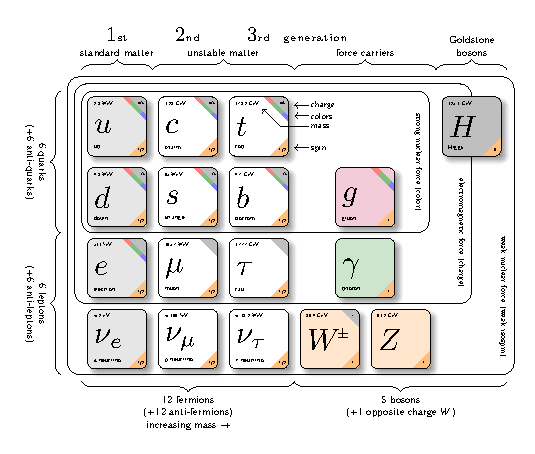
\includegraphics[width=\linewidth]{figures/SMtikz (2).pdf}
    \caption{Standard model}
    \label{fig:SMtikz}
\end{figure}
The SM 
\begin{equation}
\text{SU}(3)_C \times \text{SU}(2)_L \times \text{U}(1)_Y
\end{equation}
%Add Lagrangian
\subsection{A closer look at QCD}\label{sec1.1:ch1:QCD}
\subsection{In context}
In the context of a hadron collider, the case we are considering, there are additional non-perturbative affects that must be considered.
\section{Event Generation}\label{sec2:mc}
\subsection{}
\section{Limitations of the Standard Model and its Simulation}\label{sec3:limits}
The standard model is a "low energy" theory. Due to its perturbative nature it is only valid at a certain energy scale; in practice, after the initial collision. 

\chapter{The CMS Experiment at the Large Hadron Collider}\label{chap:cms}
The data used in this analysis is from $pp$ collisions produced by the Large Hadron Collider (LHC) and was recorded using the Compact Muon Solenoid (CMS) detector during the years 2016-2018. In this chapter, I will briefly explain the LHC complex and describe the CMS detector in detail, focusing on the subdetectors relevant to this analysis (the tracker and calorimeters).
\section{The Large Hadron Collider}
The Large Hadron Collider is the world's largest particle accelerator used for the study of proton-proton ($pp$) and heavy-ion (HIN) collisions. It is located outside of Geneva, Switzerland and its operation is overseen by the European Organization for Nuclear Research (Conseil Européen pour la Recherche Nucléaire - CERN). The LHC occupies a 26.7 km in circumference tunnel that originally housed the Large Electron-Positron (LEP) collider \cite{LEP}, and lies between 45m and 170m underground. The LHC was designed to deliver $pp$ collisions at a center of mass energy $\sqrt{s} = \sqrt{4E_{p_1}E_{p_2}}=14$ TeV and instantaneous luminosity of $\mathcal{L} = 10^{34}\mathrm{cm}^2\mathrm{s}^{-1}$ and to collide Pb ions at 2.76 GeV/nucleon at $\mathcal{L}=20^{27}\mathrm{cm}^2\mathrm{s}^-1$ and was constructed between 1998 and 2008.\\
Although we normally describe the LHC as a circular collider, it actually contains 528m long eight straight sections where the experiments and beam facilties are housed between arcs where the protons or ions are trajectories are bent.
\begin{figure}
    \centering
    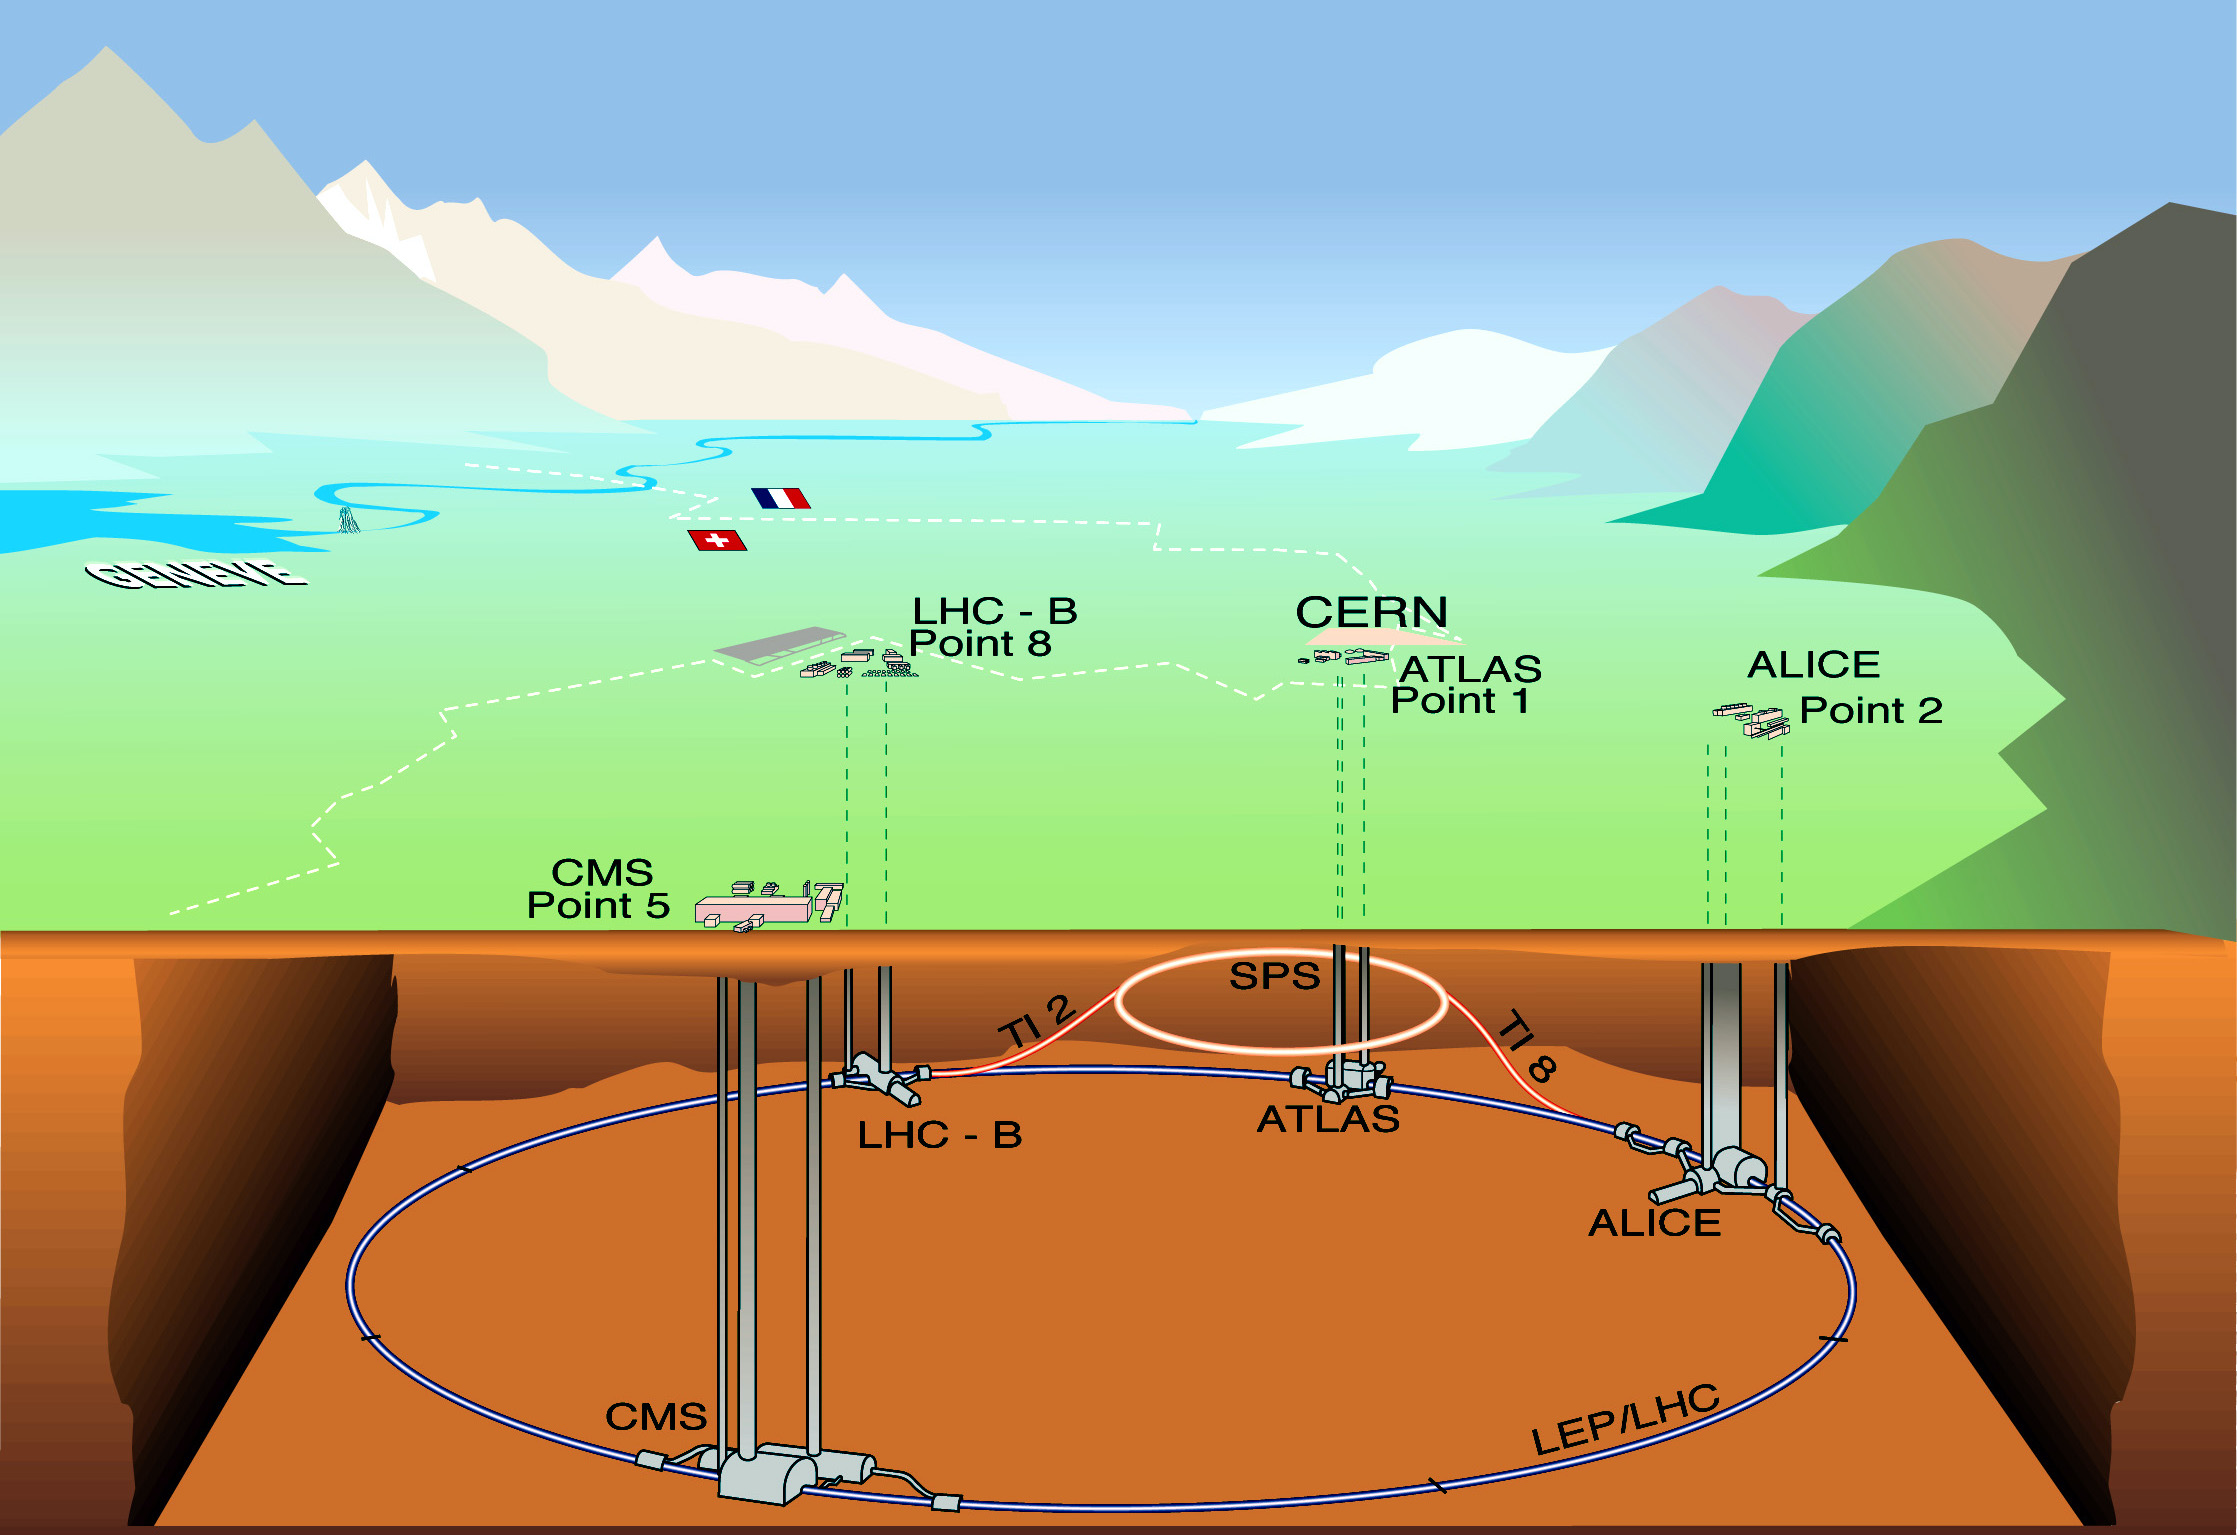
\includegraphics[width=\linewidth]{figures/LHC-PHO-1997-237.jpg}
    \caption{Schematic of the Large Hadron Collider showing its location along the French-Swiss border and where the four main detectors are located along its ring \cite{LHCMap}. }
    \label{fig:LHCmap}
\end{figure}



\section{The Compact Muon Solenoid}
\chapter{Global Event Reconstruction}\label{chap:emul}
\section{Particle Flow}
The Particle Flow algorithm is the all purpose method that is used to reconstruct events in the CMS detector of the Large Hadron Collider.
\subsection{PUPPI}
	
\section{Event and Jet Reconstruction}\label{eventsel}
In the CMS experiment, the Particle Flow (PF) algorithm \cite{particleflow} is used to reconstruct final state particles by linking information from the individual subdetectors to form a global event description. PF candidates are classified as either a muon, photon, charged hadron, or neutral hadron, ensuring that there is no double counting of of particles.
\subsection{Event Reweighting and Quality Checks}
Simulation may not accurately reflect the data due to high order effects or detector effects. To ensure that our simulation samples are representative of the data, final event counts in simulation are re-weighted to resemble the distributions observed in data. Additionally, we apply other quality checks that remove events not suitable for physics analyses due to imperfect detector conditions or poorly reconstructured variables.
\subsubsection{L1 Prefiring}\label{prefiring}
During the 2016 and 2017 data taking periods, the gradual timing shift of the ECAL was not properly propgated to the L1 trigger primitives (TP), resulting in an inefficiency for objects with $\eta > 2.0$. These high eta TPs were mistakenly associated with the previous bunch crossing; not only would this cause that trigger primitive to be missing from the correct bunch crossing, but it could cause events to self-veto if there is a significant amount ECAL energy in $2<|\eta|<3$ since L1 rules forbid two consecutive bunch crossings from firing. This effect is not described by simulations and must be accounted for by re-weighting our simulation samples. The weights are obtained by taking the product of the non-prefiring probability of all objects with overlap removal and are provided by the collaboration \cite{l1prefiring}.
\subsubsection{Primary Vertices}
Primary vertices are identified by clustering tracks based on the z-coordinate of their point of closest approach to the center of the beam spot. The clustering algorith must balance the ability to reolve nearby vertices in cases of high pileup against the possibility of splitting a single, genuine interaction vertex into more than one cluster. For this reason a deterministic annealing alogirthm is used in CMS \cite{trackPVCMS2014}. Each of the reconstructed primary vertices is then required to satisfy quality criteria: $\sqrt{x^2+y^2}<2$ cm, is not fake (i.e. is not a vertex made out of a proper fit to tracks), $\abs{z}<24$ cm, and $N_{dof} > 4$.  The primary vertex with the highest $\Sigma\pt^2$ is assigned as the leading primary vertex (PV). All other verticies are considered pileup (PU) vertices.
\subsubsection{Pileup Re-weighting}\label{PUSF}
To account for discrepancies between the pileup profile of the simulated samples and data, we apply pileup reweighting to the MC samples. The weights are determined from the ratio of the pileup distribution in data and in MC, with both distributions normalized to a unit area. The derived weights are provided by the CMS LUMI POG \cite{PUSFgithub} and are derived assuming using the full Run 2 cross-section of $\sigma_{MB}=69.2$ mb. There is a $\pm 4.6\% $ uncertainty \cite{LUMIPOGtwiki} on this cross-section measurment, and that is propagated to the weight uncertainties by scaling the cross-section up and down by this value and re-deriving the weights.
\subsubsection{2018 HEM issue}
During 2018 data-taking two HCAL modules' power supplies died, impacting the jet energy measurement in this region \cite{HEM}. In order to account for this issue we reject the event if any jet
 in the $-1.57 < \phi < -0.87$ and $-3.0 < \eta < -1.3$ region for the 2018 dataset.
\subsection{Jets}\label{jets}
Jets are reconstructed by clustering all charged PF candidates reconstructed from the primary vertex and all other neutral PF candidates. Due to its resilience against soft radiation, the anti-$k_T$ \cite{antikt} algorithm is used as the cluster jets in CMS. For this analysis that is considering the high \pt or boosted regime, we use AK8 jets, or jet's clustered using anti-$k_T$ and a radius of $R=0.8$. The pileup per particule identification (PUPPI) \cite{puppi} algorithm is use to mitgate pileup in these jets.\\
To suppress identifying jets originating from detector noise, miscalibration of detector components, or misreconstructed objets, the tight jet ID requirement \cite{jetid}. Distributions of $\eta-\phi$ for each era are shown in \ref{fig:jetvetomap} and are sufficiently flat after selections, needing no further correction or veto beyond the 2018 HEM veto.

\begin{figure}[h!]
  \centering
  \begin{subfigure}
      \centering
  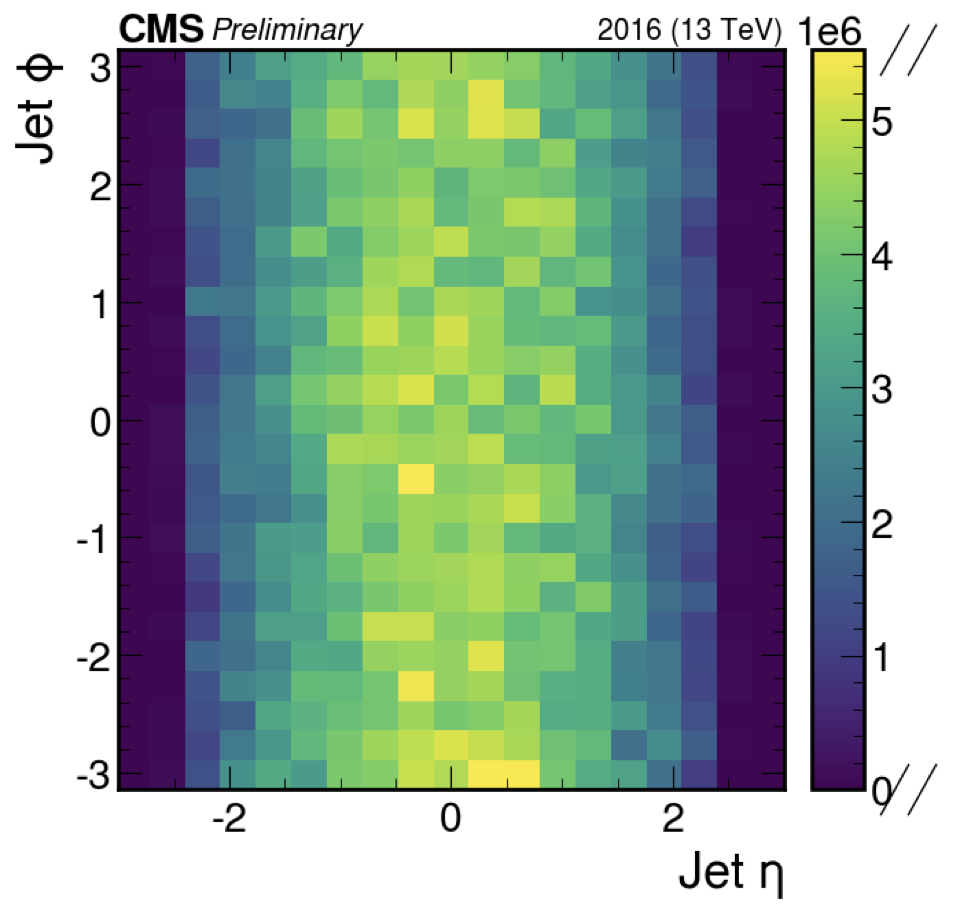
\includegraphics[width=.23\linewidth]{figures/multijet/dijet/eta_phi_2016.png}
    \end{subfigure}
    \begin{subfigure}
      \centering
      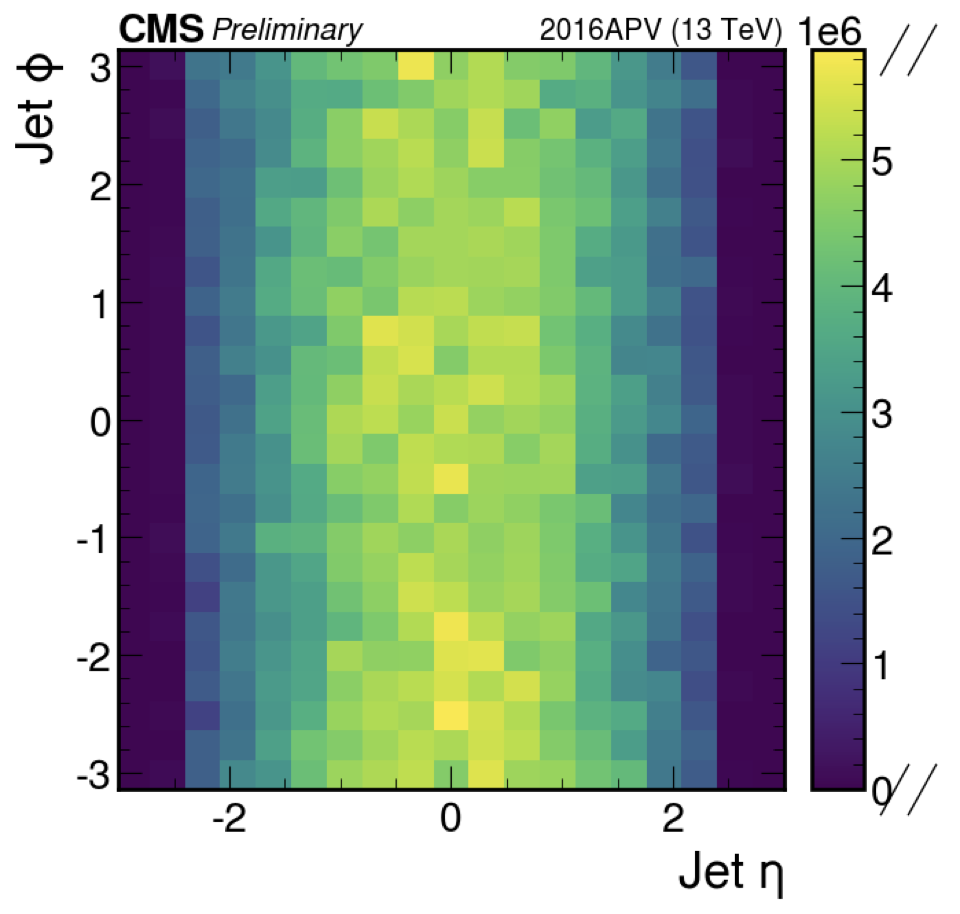
\includegraphics[width=.23\linewidth]{figures/multijet/dijet/eta_phi_2016APV.png}
    \end{subfigure}
    \begin{subfigure}
      \centering
      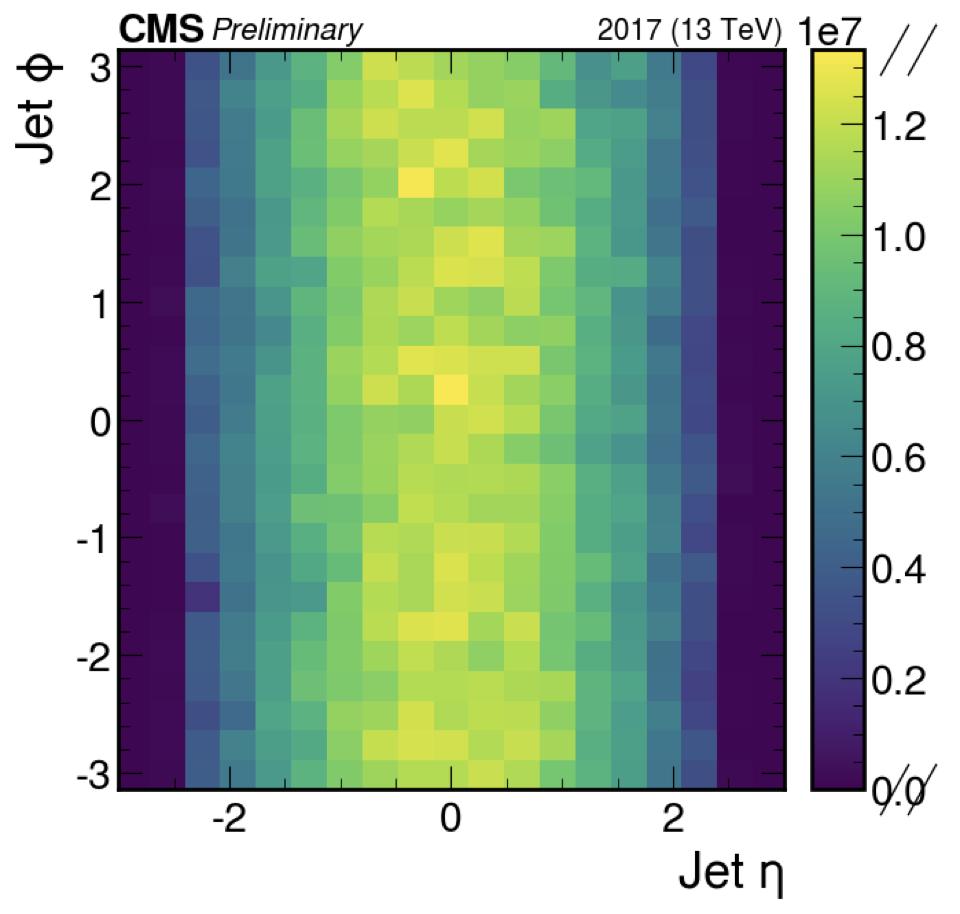
\includegraphics[width=.23\linewidth]{figures/multijet/dijet/eta_phi_2017.png}
    \end{subfigure}
    \begin{subfigure}
      \centering
      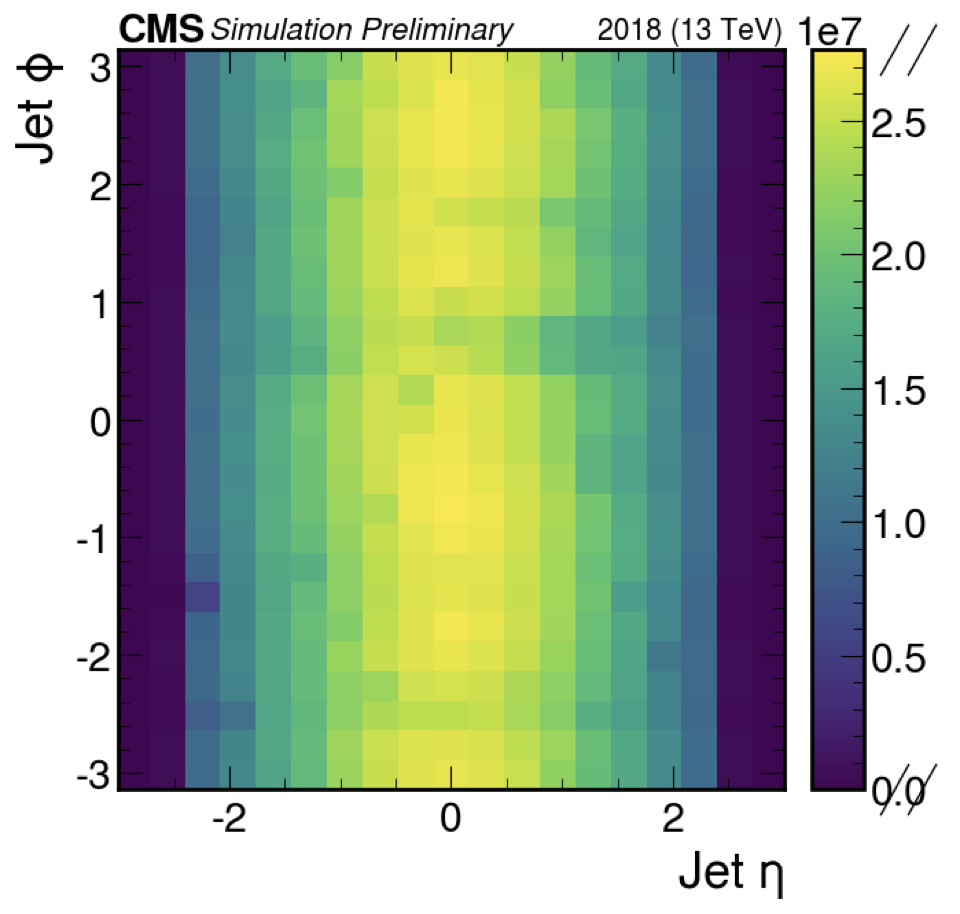
\includegraphics[width=.23\linewidth]{figures/multijet/dijet/eta_phi_2018.png}
    \end{subfigure}
    \caption{$\phi$ vs. $\eta$ distribution for each era of data taking. All are sufficiently flat to not require further veto maps, except 2018 which required the HEM veto.}
    \label{fig:jetvetomap}
\end{figure}
  
\subsubsection{Jet Energy Corrections}\label{JEC}
Kinematic observables and the reconstruction and selection efficiencies between the reconstruction of data and simulation do not agree exactly. This is to be expected since simulation is an approximation of the real world image, but to produce a reliable measurement we calibrate the jet energu and momenta to improve the agreement between data and simulation. Changing the measured value of the jets also affects the event yield after selections, so the yield in simulation is corrected to be the same as that of the data. The jet energy scales in simulation are corrected for pileup (PU) effects and differences in the momenta between data and simulation. Jets in data are additionally corrected for residual detector and reconstruction affects. The factors for the correction of the jets' momenta in data and simulation and their uncertainties are provided by the CMS collarboration as a function of \pt and $\eta$.\\
The jet \pt resolution is relatively poor compared to other physics objects; to prevent a bias from the smearing of this resolution, after JES corrections are applied, the reconstructed jet momenta is scaled so that the resolution matches that of the simulation at the particle level. For a reconstructed jet matched to a jet at the generator level, it's momentum is scaled by the factor:
\begin{equation}
  \label{eq:JER}
  c_{\textrm{JER}}=1+(s_{\textrm{JER}}-1)\frac{\pt^{\textrm{RECO}}-\pt^{\textrm{GEN}}}{\pt^{\textrm{RECO}}}
\end{equation}
The resolution scale factor $\sigma_{\textrm{JER}}$ and their corresponding uncertainties are provided by the CMS collaboration.
%Describe how JECs are applied to subjets adn softdrop mass is reconstructed from that
% Don't need PU jet id bc it's only applied to jets w/ pt below 50 GeV
% TODO: do  i need muon suppression too? or only Z+jet
% TODO : do i need MET filters?
\subsubsection{Jet Mass}
The main observables for this analysis are jet mass and \pt. The invariant jet mass is defined as
\begin{equation}
m_{j}^2 = P_\mu P^\mu  = \left(\Sigma_{i\in jet}p_i^2\right)
\end{equation}
where $P_\mu$ is the totoal four-momentum of the jet, constructed by summing the four momenta $p_i$ of all the consituents of the jet. To the first non-trivial order (NLO), for a jet originating from a massless parton, the invariant mass is:
\begin{equation}
\langle M^2\rangle  \simeq C\frac{\alpha_s}{\pi}p_T^2R^2
\end{equation}
where $C$ depends on the fraction of quarks and gluons in the jet and type of jet algorithm used \cite{jetography}. Perturbative effects from parton splitting in the soft and collinear limits and non-perturbative effects from hadronisation and underlying event are limiting factors when performing calculations of the jet mass.
% TODO: add more details about jet mass resummaton and sudakov form factors, etc... in the context of individual splittings
\subsubsection{Soft Drop Mass}
To mitigate effects from underlying event radiation, initial state radiation, and pileup, jets can be treated with grooming techniques, which aim to remove wide-angle soft  radiation from jets. CMS utilizes the soft drop algorithm \cite{softdrop} to groom jets and derive jet substructure variables such as the soft drop groomed jet mass $m_{SD}$. The soft drop algrotithm is a generalization of the modified Mass Drop Tagger (mMDT) procedure \cite{mMDT}. To perform soft drop grooming, the jets are reclustered using the Cambridge-Achen (CA) \cite{CA} clustering algorithm, and then steps backwards through it's clustering history. At each step, the two resulting subjets are compared and the softer subjet is removed until the soft drop condition is satisfied:
\begin{equation}
\frac{\min(p_{T1},p_{T2})}{p_{T1}+p_{T2}}>z_{cut}\left(\frac{\Delta R_{12}}{R_0}\right)^\beta
\end{equation}
where $p_{Ti}$ are the tranvserse momenta of the subjets w.r.t beam, $\Delta R_{12}$ is the distance between the subjets in the $\eta-\phi$ plane, $z_{cut}$ is the soft drop threshold, and $\beta$ is the angular exponent. $z_{cut}$ controls how aggressive the grooming is w.r.t \pt fraction, and in CMS is set to 0.1. The angular splitting $\beta$ reduces to the ungroomed jet when $\beta\rightarrow\infty$ and the lower the value of $\beta$, the more collinear radiation is groomed away; CMS uses a value of $\beta=0$ which reduces the procedure to mMDT and vetoes both soft and soft-collinear radiation. While the soft drop jet mass ($m_{SD}$) is IRC safe, the soft drop \pt is not IRC safe, but only Sudakov safe \cite{advancesInJet}; hence, we only use the soft drop mass as an observable along with the regular jet mass and \pt, but not the soft dropped \pt in this measurement.
% most likely will remove following section
\subsubsection{Jet Mass Scale and Resolution}\label{JMS} Just like the jet energy and momentum, the jet mass, especially for boosted jets (AK8 jets) and measurements using the softdrop mass, required corrections for a reliable comparison between data and simulated events. Jet mass scale and resolution scale factors are derived from a fit to the W-jet mass in data and simulation. These values are listed in table \ref{table:JMS} and provided by the collaboration.
\begin{table}[h!]
  \centering
\begin{tabular}{lllll}
\hline
\textbf{Year} & \textbf{JMS SF} & \textbf{JMS Unc.}         & \textbf{JMR SF} & \textbf{JMR Unc.}        \\ \hline
2016          & 1.00            &$\pm$ 0.0094 & 1.0             & $\pm$ 0.2   \\
2017          & 0.982           & $\pm$ 0.04   & 1.09            & $\pm$ 0.05  \\
2018          & 0.999           & $\pm$ 0.002  & 1.108           & $\pm$ 0.034 \\ \hline
\end{tabular}
  \caption{Jet mass scale and resolution factors and uncertainties for each era.}
  \label{table:JMS}
\end{table}

\chapter{Jet mass measurement in dijet and trijet final states}\label{chap:planner}
\section{Data and MC Samples}
\subsection{Data}\label{data}
The full Ultralegacy Run II datasets are used in this analysis. This data was taken in pp collisions in 2016, 2017, and 2018 at $\sqrt{s}=13$TeV (25 ns bunch crossings), corresponding to an integrated luminosity of 138 $\text{pb}^{-1}$. Due to differences in data-taking conditions, the dataset is split into 4 eras: 2016APV, 2016, 2017, and 2018 and correspond to integration luminosities of 19.50 $\text{pb}^{-1}$, 16.81 $\text{pb}^-1$, 41.48 $\text{pb}^{-1}$, and 59.83 $\text{pb}^{-1}$ respectively. The 2016 data is split into 2 separate datasets due to an issue in the analog pipeline voltage (APV) readout chips of the silicon strip tracker at the beginning of running in 2016. After the inefficiencies caused by this were discovered, an increase in the preamplifier feedback voltage bias (VFP) was able to recover the hit efficiency of the tracker to normal levels; however the data taken before this fix (2016APV) was already affected and mitigation of the effects was applied in offline reconstruction for it but not for those after the VFP increase (2016). \\
The data samples used and their names and eras are listed in Table \ref{table:1}. \\
Official Golden JSONs are employed to consider only the luminosity sections passing data-quality certification requirements.
\begin{itemize}
\item 2016 Data: \texttt{Cert\_271036-284044\_13TeV\_Legacy2016\_Collisions16\_JSON.txt}
\item 2017 Data: \texttt{Cert\_294927-306462\_13TeV\_UL2017\_Collisions17\_GoldenJSON.txt}
\item 2018 Data: \texttt{Cert\_314472-325175\_13TeV\_Legacy2018\_Collisions18\_JSON.txt}
\end{itemize}
% \usepackage{graphicx}
\begin{table}[h!]
	\centering
	\resizebox{\textwidth}{!}{%
		\begin{tabular}{ll}
			\hline
			Era & DAS dataset name \\ \hline
			UL2016APV B-ver1 & \texttt{/JetHT/Run2016B-ver1\_HIPM\_UL2016\_MiniAODv2\_NanoAODv9-v2/NANOAOD} \\
			UL2016APV B-ver2 & \texttt{/JetHT/Run2016B-ver2\_HIPM\_UL2016\_MiniAODv2\_NanoAODv9-v2/NANOAOD} \\
			UL2016APV C & \texttt{/JetHT/Run2016C-HIPM\_UL2016\_MiniAODv2\_NanoAODv9-v2/NANOAOD} \\
			UL2016APV D & \texttt{/JetHT/Run2016D-HIPM\_UL2016\_MiniAODv2\_NanoAODv9-v2/NANOAOD} \\
			UL2016APV E & \texttt{/JetHT/Run2016E-HIPM\_UL2016\_MiniAODv2\_NanoAODv9-v2/NANOAOD} \\
			UL2016APV F & \texttt{/JetHT/Run2016F-HIPM\_UL2016\_MiniAODv2\_NanoAODv9-v2/NANOAOD} \\ \hline
			UL2016 F & \texttt{/JetHT/Run2016F-UL2016\_MiniAODv2\_NanoAODv9-v1/NANOAOD} \\
			UL2016 G & \texttt{/JetHT/Run2016G-UL2016\_MiniAODv2\_NanoAODv9-v1/NANOAOD} \\
			UL2016 H & \texttt{/JetHT/Run2016H-UL2016\_MiniAODv2\_NanoAODv9-v1/NANOAOD} \\ \hline
			UL2017 B & \texttt{/JetHT/Run2017B-UL2017\_MiniAODv2\_NanoAODv9-v1/NANOAOD} \\
			UL2017 C & \texttt{/JetHT/Run2017C-UL2017\_MiniAODv2\_NanoAODv9-v1/NANOAOD} \\
			UL2017 D & \texttt{/JetHT/Run2017D-UL2017\_MiniAODv2\_NanoAODv9-v1/NANOAOD} \\
			UL2017 E & \texttt{/JetHT/Run2017E-UL2017\_MiniAODv2\_NanoAODv9-v1/NANOAOD} \\
			UL2017 F & \texttt{/JetHT/Run2017F-UL2017\_MiniAODv2\_NanoAODv9-v1/NANOAOD} \\ \hline
			UL2018 A & \texttt{/JetHT/Run2018A-UL2018\_MiniAODv2\_NanoAODv9-v2/NANOAOD} \\
			UL2018 B & \texttt{/JetHT/Run2018B-UL2018\_MiniAODv2\_NanoAODv9-v1/NANOAOD} \\
			UL2018 C & \texttt{/JetHT/Run2018C-UL2018\_MiniAODv2\_NanoAODv9-v1/NANOAOD} \\
			UL2018 D & \texttt{/JetHT/Run2018D-UL2018\_MiniAODv2\_NanoAODv9-v2/NANOAOD} \\ \hline
		\end{tabular}%
	}\caption{Full Run 2 Ultra Legacy datasets used in this analysis. }
\label{table:1}
\end{table}
\subsection{Monte Carlo Simulation}\label{MC}
The simulation of the pp collision events is performed using various Monte Carlo (MC) software packages in multiple steps. The matrix-element generation for the samples used in the analyses is handled by MADGRAPH5 aMC@NLO v2.6.5 (v2.6.1) \cite{madgraph}. The samples are then interfaced with PYTHIA 8.244 \cite{pythia8} for parton showering and hadronization. All samples used in this dataset and their cross-sections are show in Table \ref{table:2}.\\
All samples were generated using PYTHIA8 settings; in them the CP5 tune \cite{CP5} is used and NNPDF3.1 \cite{nnpdf} PDF sets for the modeling of the parton distribution functions are used. The generated events are then passed through the GEANT4 \cite{geant4} package to simulate the detector response before they are treated with the same reconstruction algorithms as the real data. As a cross-check and for calculation of the parton shape and scale uncertainties, additional samples of MADGRAPH interfaced with HERWIG7 \cite{herwig}  with tune CH3 are used. These samples are shown in Table \ref{table:3}.\\
% TODO -- what are the exact versions of madgraph and pythia used in these MC samples and is it NNNPDF3.1 used?
\begin{table}[h!]
	\centering
	\resizebox{\textwidth}{!}{%
		\begin{tabular}{ll}
			\hline
			DAS Dataset & XS \\ \hline
			\texttt{QCD\_HT200to300\_TuneCP5\_PSWeights\_13TeV-madgraphMLM-pythia8} & 1554000.0 \\
			\texttt{QCD\_HT300to500\_TuneCP5\_PSWeights\_13TeV-madgraphMLM-pythia8} & 323800.0  \\
			\texttt{QCD\_HT500to700\_TuneCP5\_PSWeights\_13TeV-madgraphMLM-pythia8} & 30280.0 \\
			\texttt{QCD\_HT700to1000\_TuneCP5\_PSWeights\_13TeV-madgraphMLM-pythia8} & 6392.0 \\
			\texttt{QCD\_HT1000to1500\_TuneCP5\_PSWeights\_13TeV-madgraphMLM-pythia8} & 1118.0 \\
			\texttt{QCD\_HT1500to2000\_TuneCP5\_PSWeights\_13TeV-madgraphMLM-pythia8} & 108.9 \\
			\texttt{QCD\_HT2000toInf\_TuneCP5\_PSWeights\_13TeV-madgraphMLM-pythia8} & 21.93  \\ \hline
		\end{tabular}%
	}\caption{Madgraph MLM + Pythia8 datasets and cross sections.
}\label{table:2}
\end{table}
\begin{table}[h!]
	\centering
	\resizebox{\textwidth}{!}{%
		\begin{tabular}{ll}
			\hline
			DAS Dataset & XS \\ \hline
			\texttt{QCD\_HT200to300\_TuneCH3\_13TeV-madgraphMLM-herwig7} & 883.5 \\
			\texttt{QCD\_HT300to500\_TuneCH3\_13TeV-madgraphMLM-herwig7} & 259.6  \\
			\texttt{QCD\_HT500to700\_TuneCH3\_13TeV-madgraphMLM-herwig7} & 23.63 \\
			\texttt{QCD\_HT700to1000\_TuneCH3\_13TeV-madgraphMLM-herwig7} & 4.943 \\
			\texttt{QCD\_HT1000to1500\_TuneCH3\_13TeV-madgraphMLM-herwig7} & 0.8013  \\
			\texttt{QCD\_HT1500to2000\_TuneCH3\_13TeV-madgraphMLM-herwig7} & 0.06815\\
			\texttt{QCD\_HT2000toInf\_TuneCH3\_13TeV-madgraphMLM-herwig7} & 0.01245 \\ \hline
		\end{tabular}%
	}\caption{Madgraph MLM + HERWIG7 and cross sections.}\label{table:3}
\end{table}
\section{Event Selection}
This section describes how events are selected at the trigger and particle level.
\subsection{Trigger Selection}
% TODO: add more information about how triggers fire
The data used for the dijet and trijet analyses are collected using single jet triggers at the High Level Trigger (HLT) that trigger based on the jet's transverse momentum. The L1 and HLT thresholds for each of the triggers are listed in table \ref{table:tab1}. As done in Ref. \cite{1605_IncJet}, we divide the events into independent regions as a function of leading jet \pt. In each region only one trigger is used and there is no overlap between regions to avoid double counting. The regions are chosen so that each trigger assigned to it is fully efficient. The edges of the trigger regions are then also used as the \pt bin edges for the jet cross sections so no \pt bin has more than one trigger.\\
The trigger efficiencies are calculated using the emulator method, where the trigger decision is emulated in data using the trigger objects of a reference trigger, trig\textsubscript{ref}. To reproduce the trigger decision, objects from both trigger levels are needed, L1 and HLT. Under the assumption that the reference trigger is fully efficient for the considered phase space of the desired trigger, the efficiency is defined as:
\begin{equation}\label{eq:1}
\epsilon_{{\rm trig_i}}=\frac{\rm Events\left({\rm L1Object}\_\pt>\pt_{{\rm ref}}\quad \& \quad {\rm HLTObject\_\pt>\pt_i \quad\&\quad trig_{ref}} \right)} { \rm Events \left( trig_{ref} \right) }
\end{equation}
where trig\textsubscript{i} is the trigger of interest. For example, if we wanted to calculate the effciency of the HLTPFJetAK8\_200 trigger, we would find the number of events that passed the reference trigger, HLTPFJetAK8\_140, have an L1 seed \pt greater than the reference trigger's, L1Object\_\pt\textgreater140, and an HLT object \pt greater than the trigger in question, HLTObject\_\pt\textgreater200. Then divide this by the total number of events that pass trig\textsubscript{ref}. The complete list of triggers with their reference triggers and L1 and HLT threshold \pt's are shown in Table \ref{table:tab1}.\\
\begin{table}[h!]
  \centering
	\resizebox{\textwidth}{!}{%
		\begin{tabular}{@{}llllllll@{}}
			\hline
			Trigger & Reference Trigger & \begin{tabular}[c]{@{}l@{}} L1 Threshold\\ (GeV) \end{tabular} & \begin{tabular}[h!]{@{}l@{}} HLT Threshold \\ (GeV)\end{tabular} & \begin{tabular}[c]{@{}l@{}}Full efficiency \\ threshold 2016 \\ (GeV)\end{tabular} & \begin{tabular}[c]{@{}l@{}}Full efficiency \\ threshold 2016APV \\ (GeV)\end{tabular} & \begin{tabular}[c]{@{}l@{}}Full efficiency \\ threshold 2017 \\ (GeV)\end{tabular} & \begin{tabular}[c]{@{}l@{}}Full efficiency\\ threshold 2018 \\ (GeV)\end{tabular} \\ \hline
			HLT\_AK8PFJet60 & HLT\_AK8PFJet40 & 0 & 60 & 178 & 0 & 0 & 0 \\
			HLT\_AK8PFJet80 & HLT\_AK8PFJet60 & 60 & 80 & 205 & 181 & 168 & 177 \\
			HLT\_AK8PFJet140 & HLT\_AK8PFJet80 & 80 & 140 & 295 & 295 & 267 & 281 \\
			HLT\_AK8PFJet200 & HLT\_AK8PFJet140 & 140 & 200 & 379 & 389 & 359 & 394 \\
			HLT\_AK8PFJet260 & HLT\_AK8PFJet200 & 200 & 260 & 459 & 463 & 447 & 484 \\
			HLT\_AK8PFJet320 & HLT\_AK8PFJet260 & 260 & 320 & 544  & 554 & 537 & 570 \\
			HLT\_AK8PFJet400 & HLT\_AK8PFJet360 & 320 & 400 & 643 & 664 & 646 & 683 \\
			HLT\_AK8PFJet450 & HLT\_AK8PFJet440 & 400 & 450 & 702 & 733 & 718 & 751 \\
			HLT\_AK8PFJet500 & HLT\_AK8PFJet530 & 450 & 500 & 802 & 838 & 791 & 817 \\
			HLT\_AK8PFJet550 & HLT\_AK8PFJet630 & 500 & 550 & N/A & N/A & 887 & 884 \\ \hline
		\end{tabular}
		%
	}
\caption{List of available triggers for our \pt range with corresponding reference triggers, and their \pt thresholds at L1 and HLT. The \pt threshold corresponding to the starting point of full efficiency is also specified for each trigger and year.}
\label{table:tab1}
\end{table}
Each trigger has a turn-on curve, and the \pt at which these curves plateau, and the trigger becomes fully efficient ($>$ 0.99), can be derived from a fit using the following equation:
\begin{equation} \label{eq:2}
%\epsilon = 0.5*\left(1+\textrm{erf}\left(\frac{x-b}{\sqrt{2}c} \right)\right)
%  \epsilon = a+0.5(1-a)\left(1+\textrm{erf}\left(\frac{x-b}{c} \right)\right)
  \epsilon = a\left(b+\frac{1-b}{2}\left(1-\text{erf}\left(\frac{x-c}{d}\right)\right)\right)
\end{equation}
where b and c are free parameters. Figure \ref{fig:4} shows the results of this fit to the efficiency as a function of \pt for trigger HLTPFJetAK8\_200 trigger, and the threshold \pt, which is found by inverting Eq. \ref{eq:1} and setting it equal to 0.99. The plots for the rest of the available triggers can be found in the Appendix.
\begin{equation}
\pt  =c+d*\text{erf}^{-1}(1-((0.99/a - b)/(0.5*(1-b))))
\end{equation}
The resulting turn-on \pt's are used to assign the correct trigger and corresponding prescale to that event. Continuing our previous example, if a 2016 event has passed the HLTPFJetAK8\_200 trigger, and has a leading jet \pt between 459 GeV and 544 GeV (see tab. \ref{table:tab1}, that event will be assigned the trigger HLTPFJetAK8\_200 and its corresponding prescale.
\begin{figure}[h!]
	\centering
	\begin{subfigure}
		\centering
		\includegraphics[width=0.45\textwidth]{figures/multijet/2016APV_trig_eff/efficiency_HLT_AK8PFJet200.png}
	\end{subfigure}%
	\begin{subfigure}
		\centering
		\includegraphics[width=0.45\textwidth]{figures/multijet/2016_trigg_eff/efficiency_HLT_AK8PFJet200.png}
	\end{subfigure}
	\begin{subfigure}
		\centering
		\includegraphics[width=0.45\textwidth]{figures/multijet/2017_trig_eff/efficiency_HLT_AK8PFJet200.png}
	\end{subfigure}%
	\begin{subfigure}
		\centering
		\includegraphics[width=0.45\textwidth]{figures/multijet/2018_trig_eff/efficiency_HLT_AK8PFJet200.png}
	\end{subfigure}
	\caption{HLT\_AK8PFJet200 Trigger efficiencies for 2016APV (top left), 2016 (top right), 2017 (bottom left), and 2018 (bottom right).}
	\label{fig:4}
\end{figure}
The trigger prescale values vary from run to run and even from lumisection to lumisection. All of the trigger values are available in brilcalc TRG \cite{brilcalc}, and we use the event pt, run information, and lumisection to map it to the correct prescale value before applying it. The trigger path assignment and prescale application is illustrated in figure \ref{fig:trigstitch}. Once the correct prescale for each event has been found, it is stored as an event weight.
\begin{figure}[h!]
  \begin{subfigure}
	\centering
	\includegraphics[width=0.9\textwidth]{figures/multijet/2016APV_TrigPlots.png}
\end{subfigure}
\begin{subfigure}
	\centering
	\includegraphics[width=0.9\textwidth]{figures/multijet/2016_TrigPlots.png}
\end{subfigure}
\begin{subfigure}
	\centering
	\includegraphics[width=0.9\textwidth]{figures/multijet/2017_TrigPlots.png}
\end{subfigure}
\begin{subfigure}
	\centering
	\includegraphics[width=0.9\textwidth]{figures/multijet/2018_TrigPlots.png}
\end{subfigure}
	\caption{All trigger paths available for all events (left), all trigger paths with prescales applied (center), all events sorted by trigger path with prescales applied and doubled events removed (right) for 2016, 2016APV, 2017, and 2018}
	\label{fig:trigstitch}
      \end{figure}
The turn-on \pt's are also used to select the \pt binning for the final measurement. Since we are combining all of the data-taking eras into one final result, for simplicity we take an approximation of the largest turn-on \pt for each trigger for the final \pt binning of [200, 290, 400, 480, 570, 680, 760, 840, 890, $\inf$]. Since there are substantially fewer events in the 840 and 890 GeV bins, we combine them together with the $\inf$ bin for an initial \pt binning of  [200, 290, 400, 480, 570, 680, 760, 840, 890, $\inf$] that is further  optimized for unfolding in section \ref{unfolding}.
\subsection{Jet selection}\label{selection}
The events selected by the triggers described above are then used in the full selections for the dijet and trijet events. The dijet selection is based on previous analyses \cite{1605_IncJet}, \cite{dijetZjet2013} and prioritize a back-to-back topology, while the trijet selection  has been optimized to increase gluon selection based on Ref. \cite{pureSamples}. All jets used are AK8 jets reconstructed as described in section \ref{jets} and passing the tight jet id criteria \cite{jetid}. %describe tight jet criteria??
For the dijet events, we require:
\begin{itemize}
	\item At least two jets with \pt\textgreater\, 200 GeV and $y < 2.5$,
	\item $\Delta\phi < 2.0$ and $\pt_{assym}<0.3$ between the leading two jets,
\end{itemize}
and select the two leading jets within each event.
For the trijet events we require:
\begin{itemize}
	\item At least three jets with \pt\textgreater\, 200 GeV and $y < 2.5$,
	\item $\Delta\phi < 1.0$ between each of the leading three jets,
\end{itemize}
and select the third softest jet of each event, as this is the jet most likely to be gluon-initiated.
% Describe jet veto maps
Figures \ref{fig:15} and \ref{fig:16} show the Data to MC agreement after selection. In these plots, the MG+Pythia8 distribution are scaled to the integral of the data. The considerable data to MC disagreement stems from the difficulty to model multijet QCD events in simulation. Figures \ref{fig:17} and \ref{fig:18} show the agreement between data and simulation for the ungroomed and groomed mass within each final \pt bin chosen for unfolding for dijet events, repsectively.  SImilarly, figures \ref{fig:19} and \ref{fig:20} show the agreement between data and simulation forthe ungroomed and groomed mass within each final \pt bin chosen for unfolding for the trijet events. Again, the simulation distributions are scaled to the integral of the data distirbution, but now normalised within each \pt bin.
\begin{figure}[h!]
  \centering
  \begin{subfigure}
    \centering
    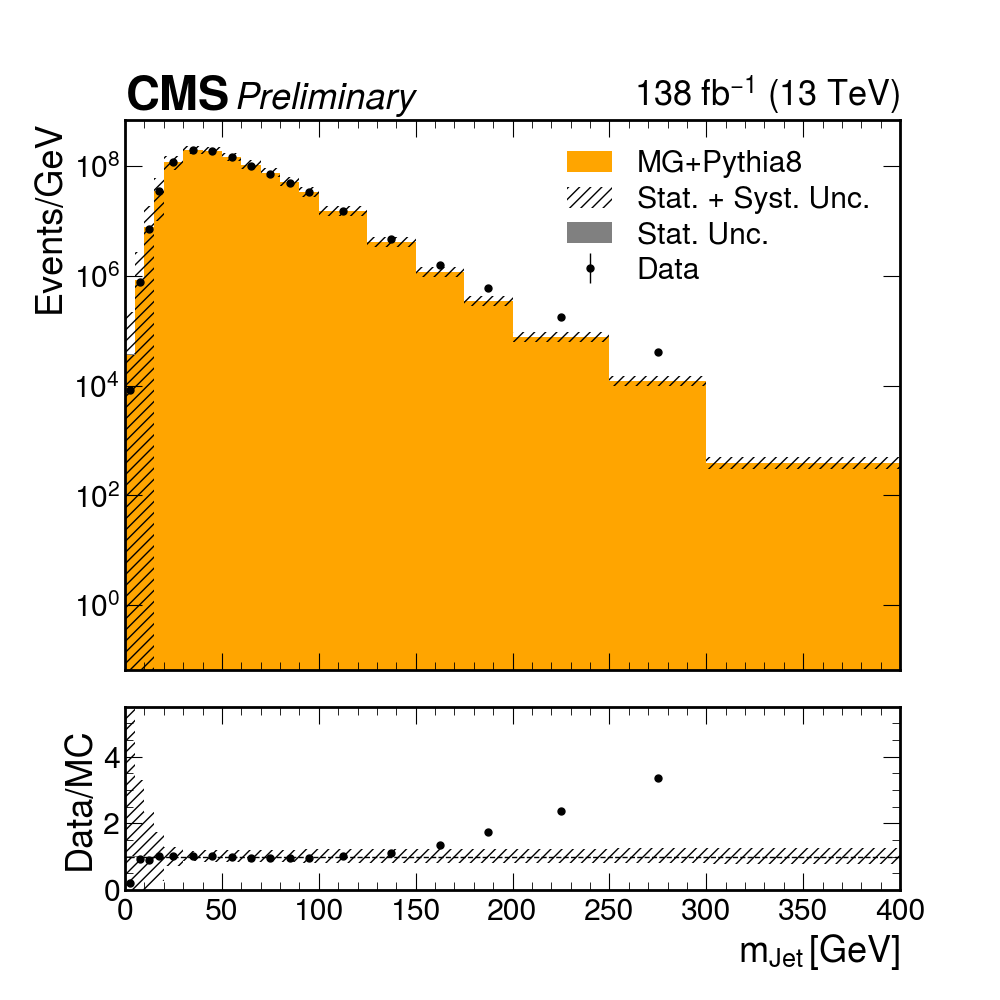
\includegraphics[width=0.45\textwidth]{figures/multijet/dijet/mjet_allyears_coarsebin.png}
  \end{subfigure}
  \begin{subfigure}
    \centering
    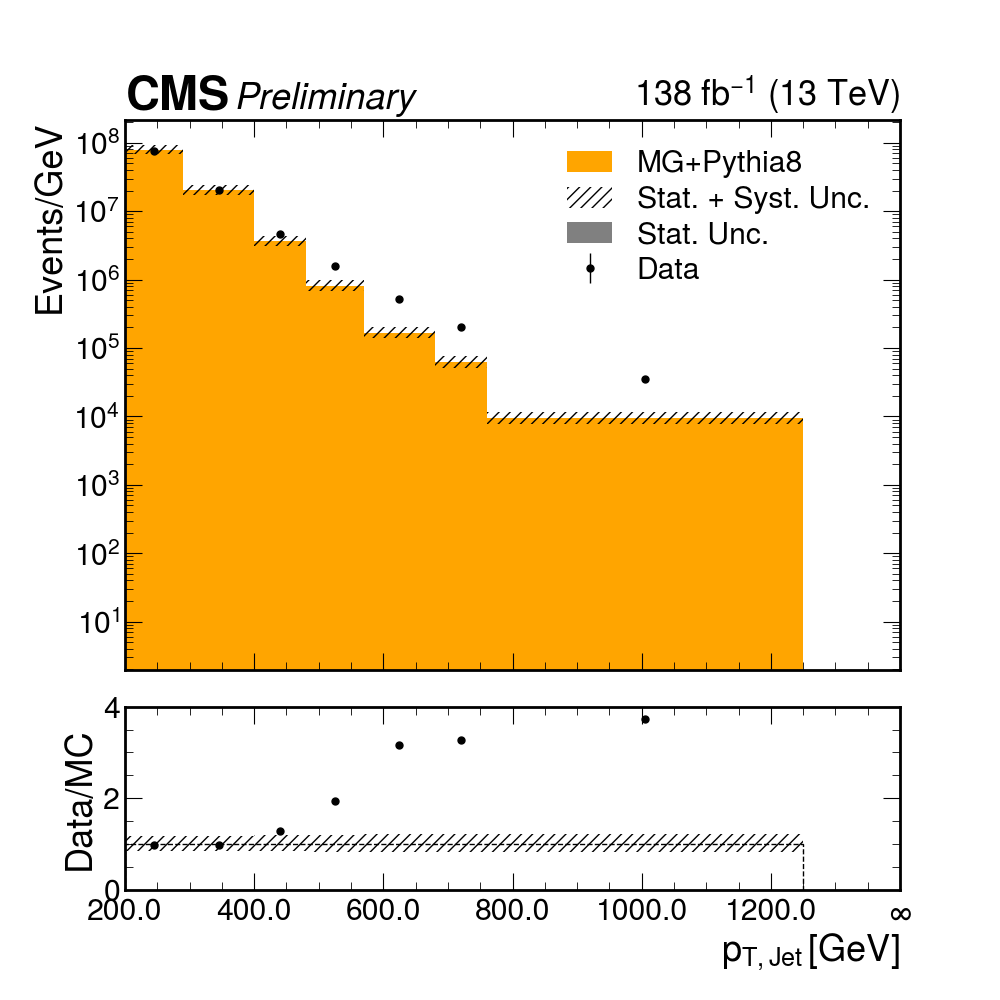
\includegraphics[width=0.45\textwidth]{figures/multijet/dijet/pt_allyears_coarsebin.png}
  \end{subfigure}
  \begin{subfigure}
    \centering
    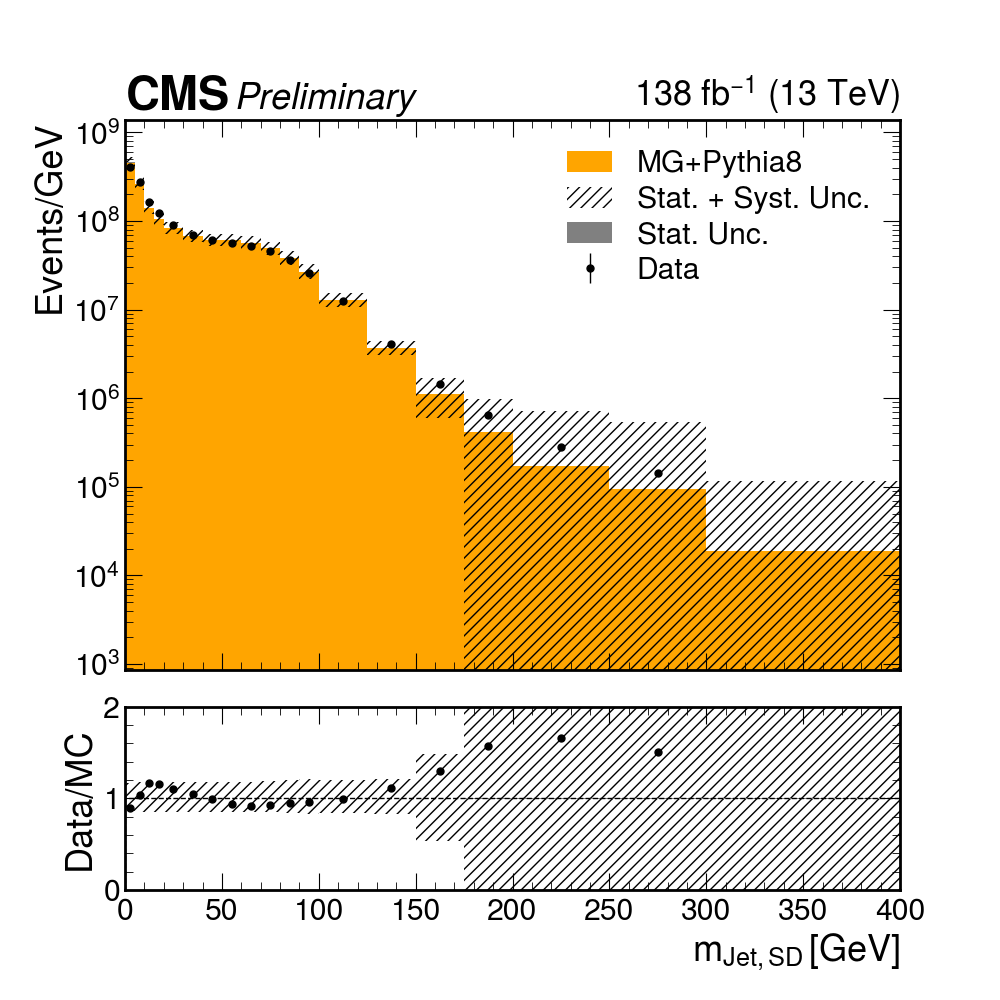
\includegraphics[width=0.45\textwidth]{figures/multijet/dijet/msd_allyears_coarsebin.png}
  \end{subfigure}
  \begin{subfigure}
    \centering
    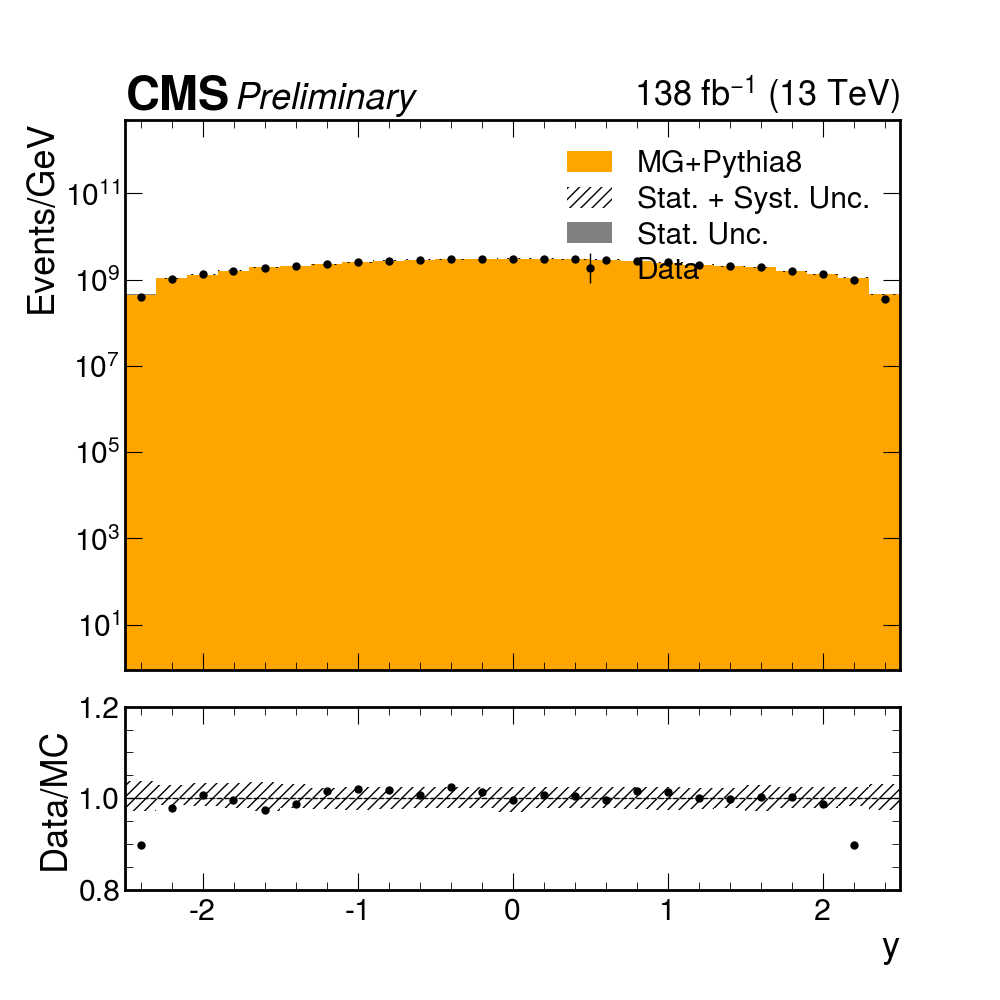
\includegraphics[width=0.45\textwidth]{figures/multijet/dijet/rap_allyears_coarsebin.png}
  \end{subfigure}
  \begin{subfigure}
    \centering
    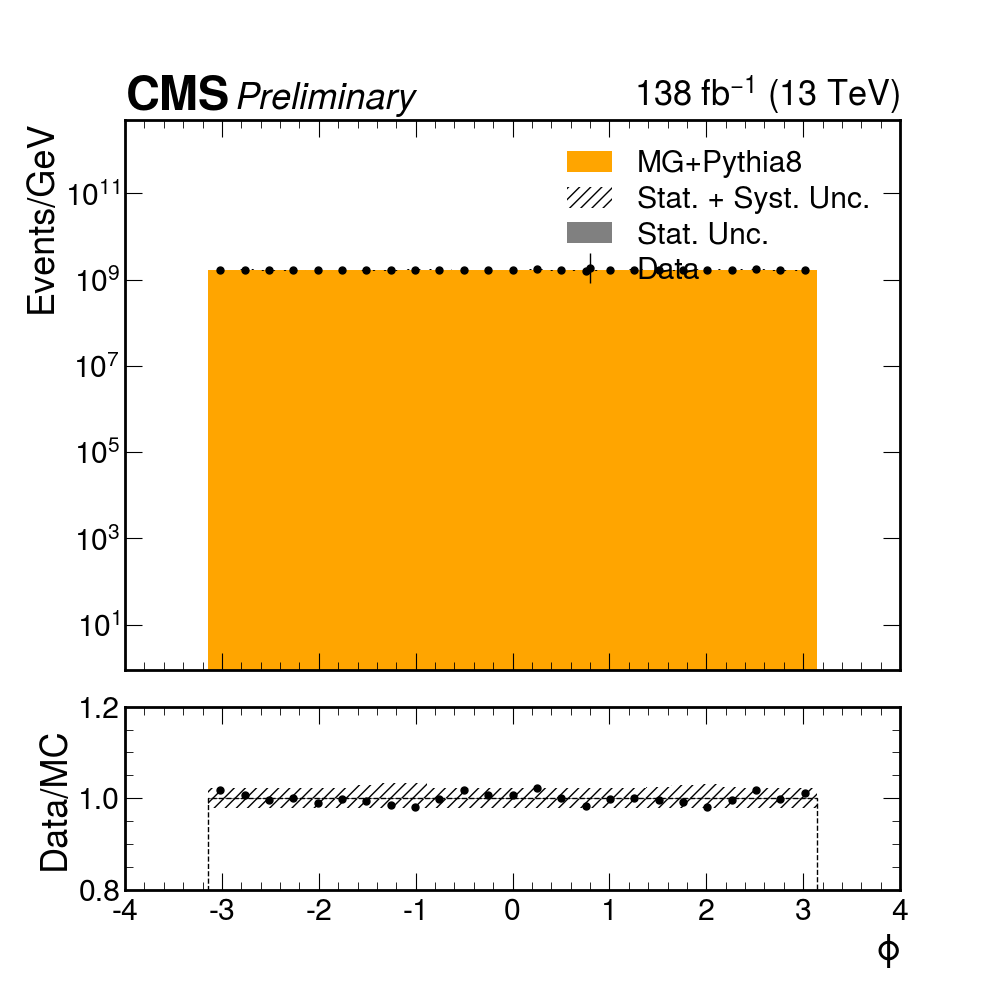
\includegraphics[width=0.45\textwidth]{figures/multijet/dijet/phi_allyears_coarsebin.png}
  \end{subfigure}
  \caption{Full Run 2 UL dijet Data to MC comparison for ungroomed mass (top left), transverse momentum (top right), softdrop mass (center left), rapidity (center right), and phi (bottom).}
	\label{fig:15}
\end{figure}
\begin{figure}[h!]
  \centering
  \begin{subfigure}
    \centering
    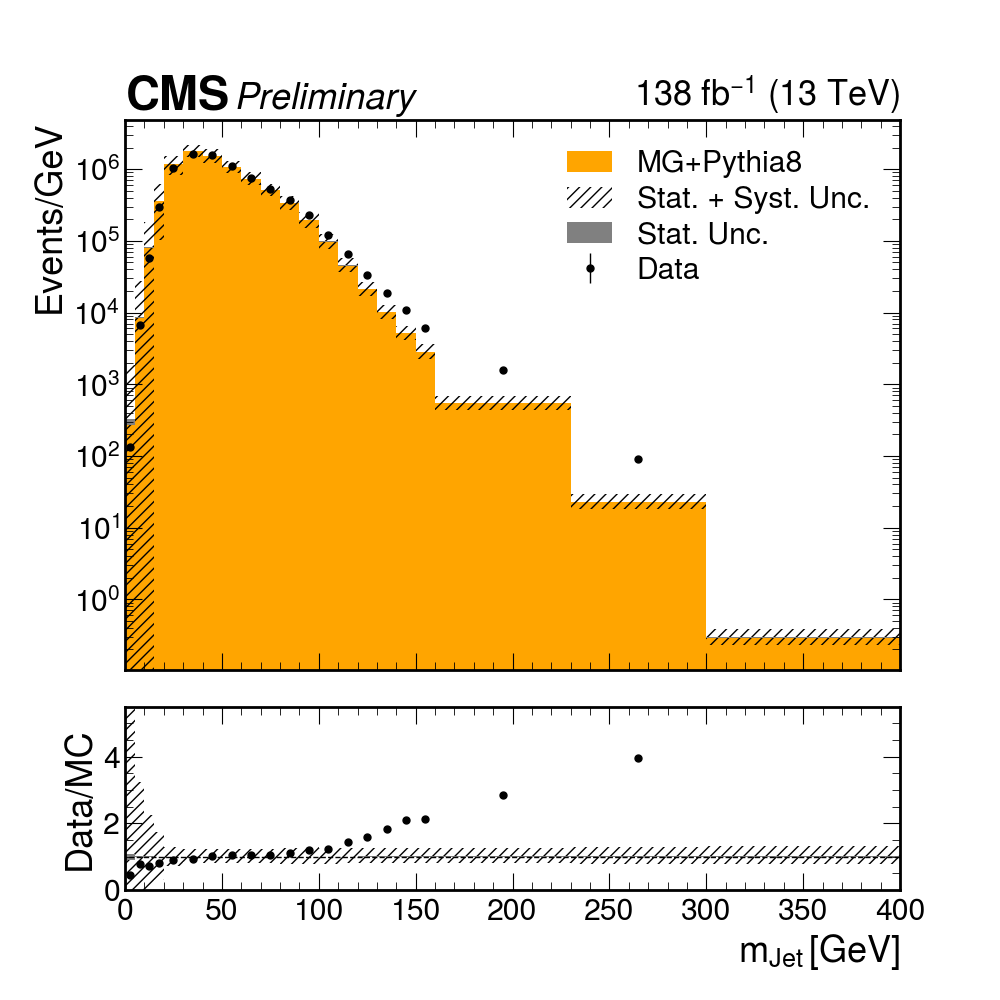
\includegraphics[width=0.45\textwidth]{figures/multijet/trijet/mjet_allyears_coarsebin.png}
  \end{subfigure}
  \begin{subfigure}
    \centering
    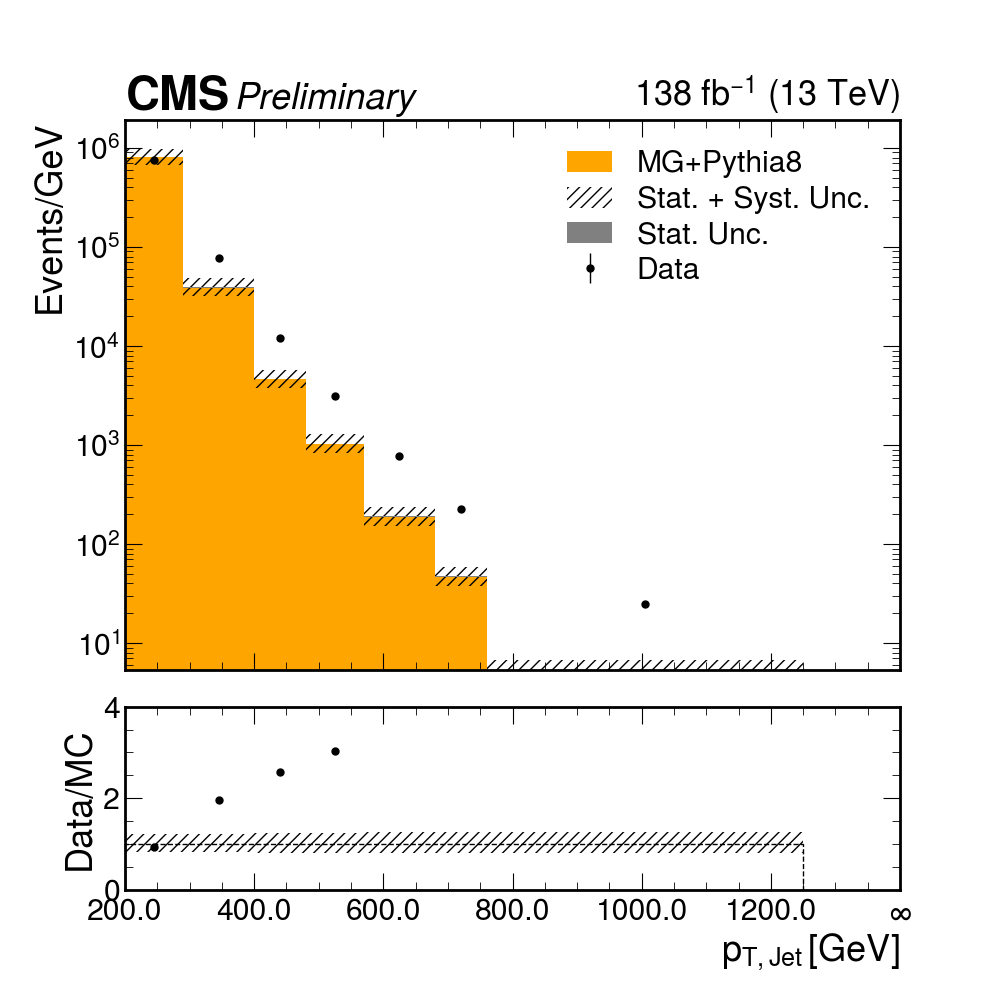
\includegraphics[width=0.45\textwidth]{figures/multijet/trijet/pt_allyears_coarsebin.png}
  \end{subfigure}
  \begin{subfigure}
    \centering
    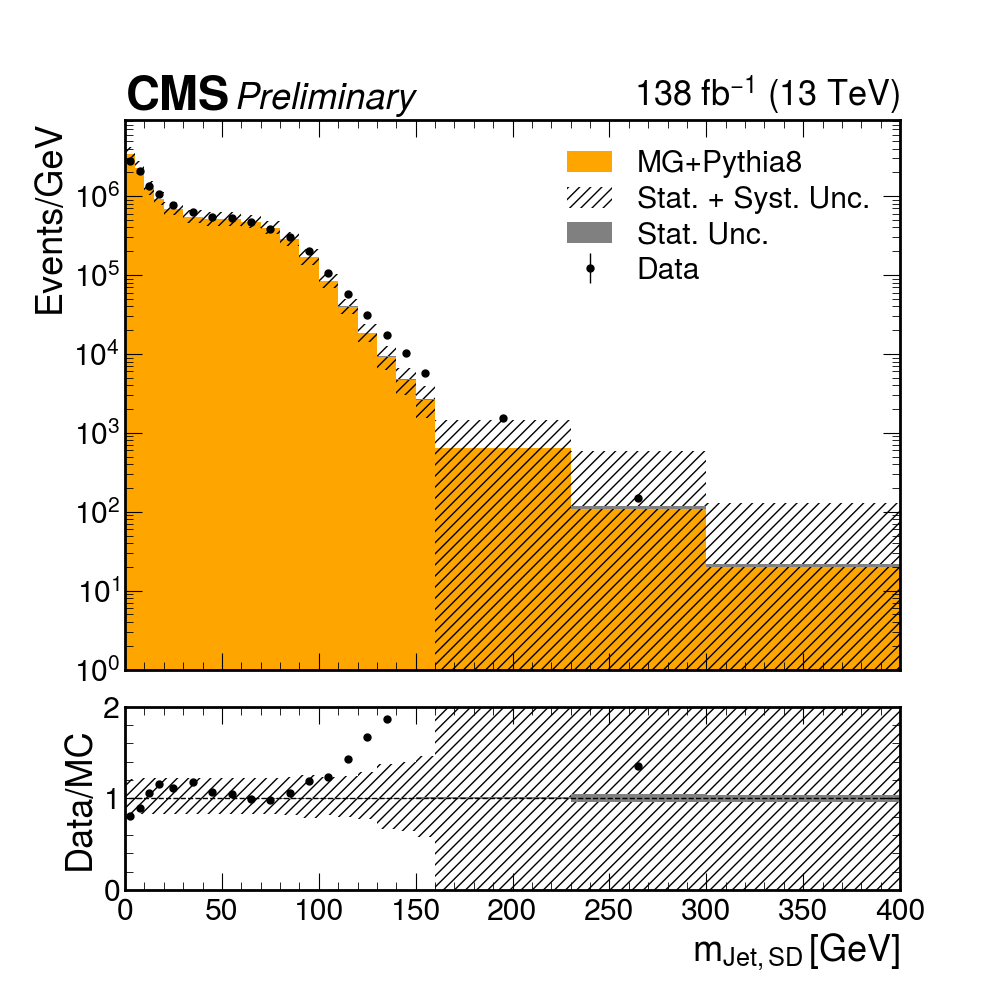
\includegraphics[width=0.45\textwidth]{figures/multijet/trijet/msd_allyears_coarsebin.png}
  \end{subfigure}
  \begin{subfigure}
    \centering
    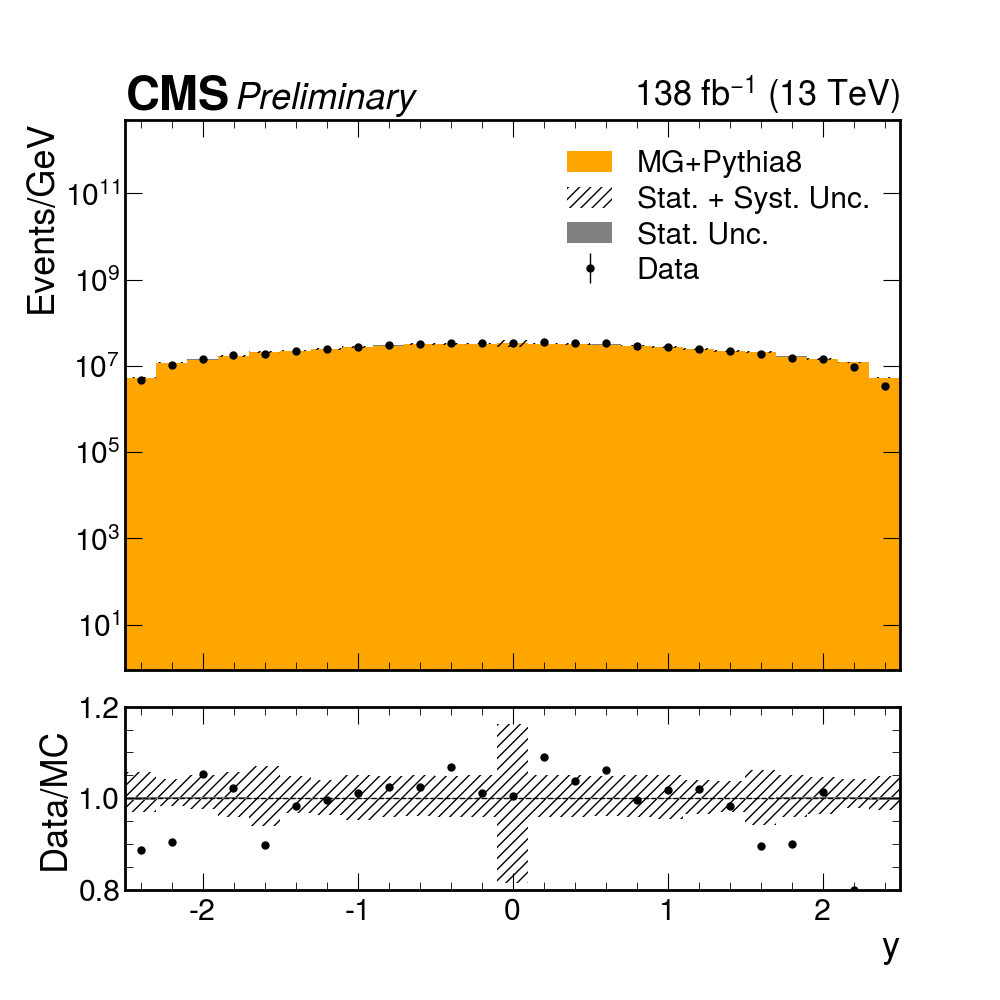
\includegraphics[width=0.45\textwidth]{figures/multijet/trijet/rap_allyears_coarsebin.png}
  \end{subfigure}
  \begin{subfigure}
    \centering
    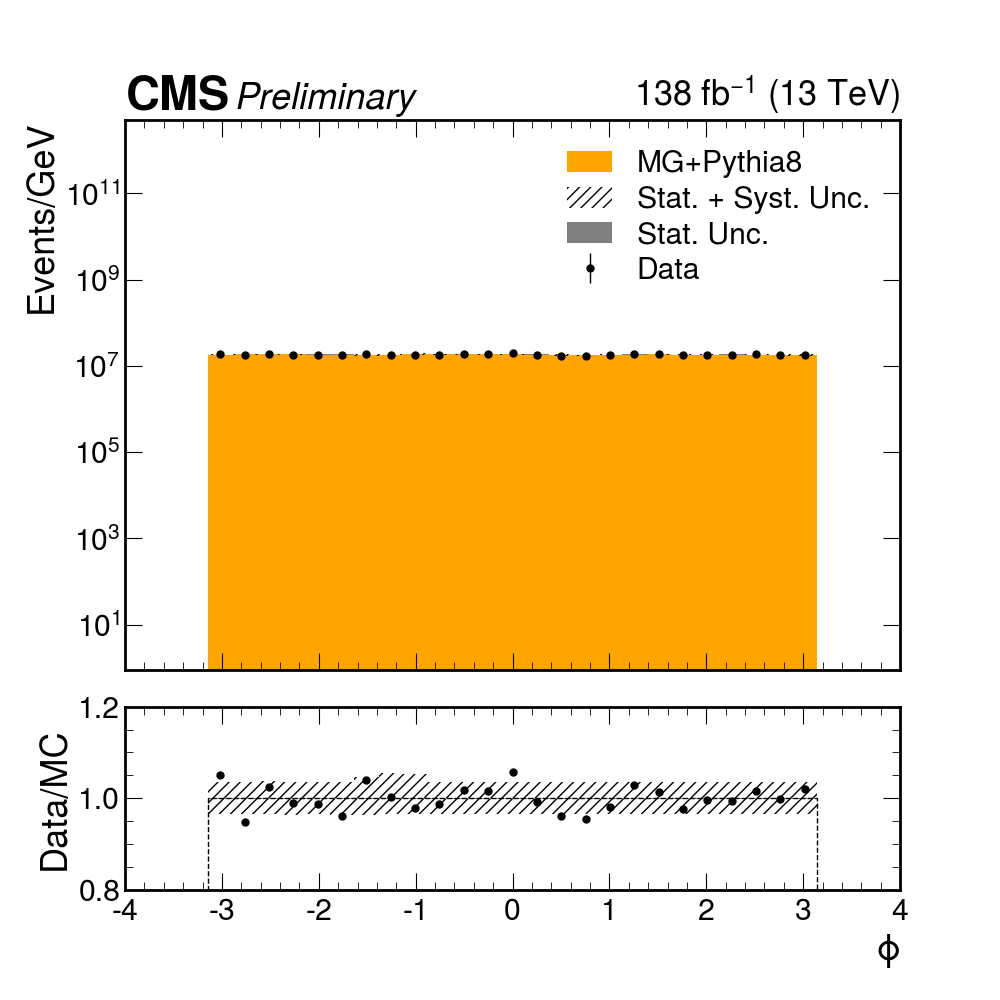
\includegraphics[width=0.45\textwidth]{figures/multijet/trijet/phi_allyears_coarsebin.png}
  \end{subfigure}
  \caption{Full Run 2 UL trijet Data to MC comparison for ungroomed mass (top left), transverse momentum (top right), softdrop mass (center left), rapidity (center right), and phi (bottom).}
  \label{fig:16}
\end{figure}
\begin{figure}[h!]
  \centering
  \begin{subfigure}
    \centering
    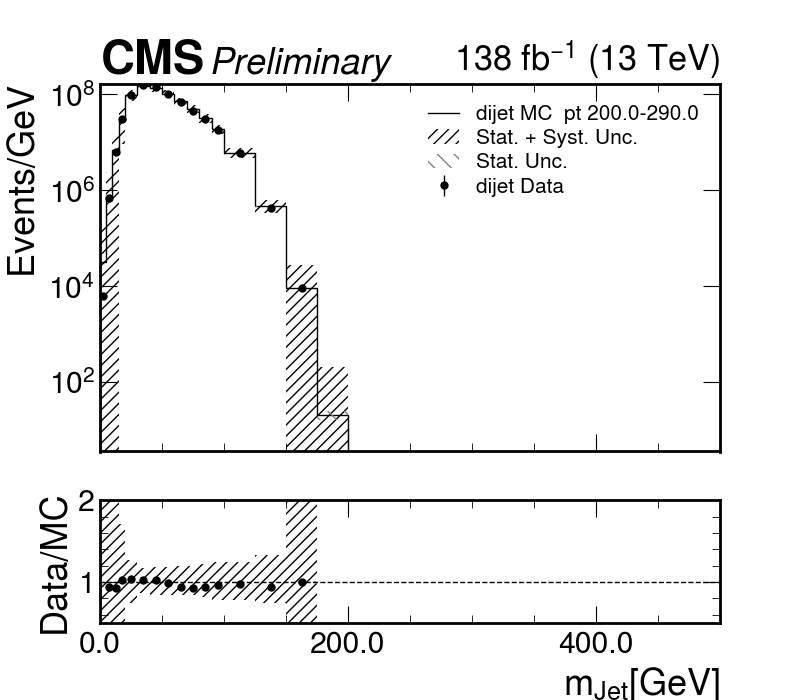
\includegraphics[width=0.45\textwidth]{figures/multijet/dijet/dijet_m_200_290.png}
  \end{subfigure}
  \begin{subfigure}
    \centering
    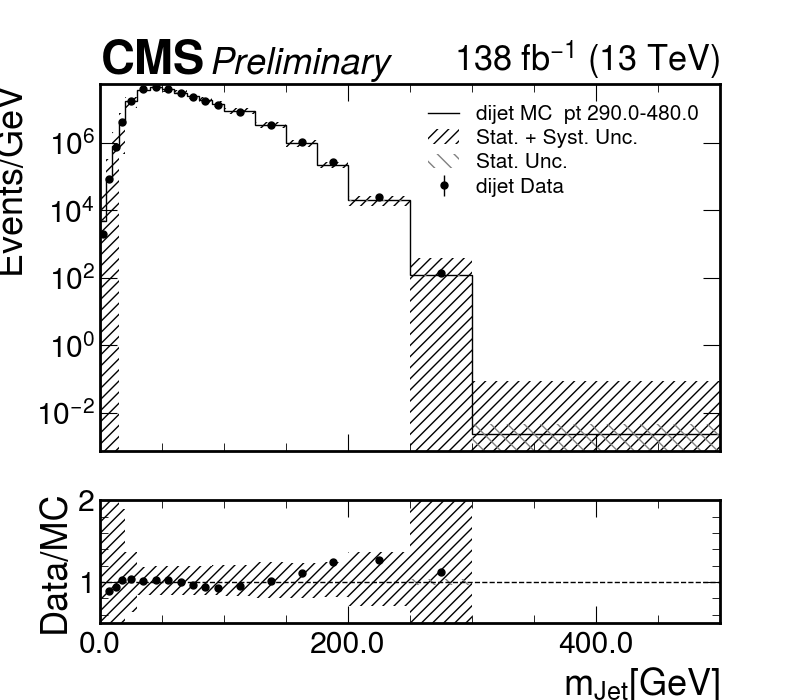
\includegraphics[width=0.45\textwidth]{figures/multijet/dijet/dijet_m_290_480.png}
  \end{subfigure}
  \begin{subfigure}
    \centering
    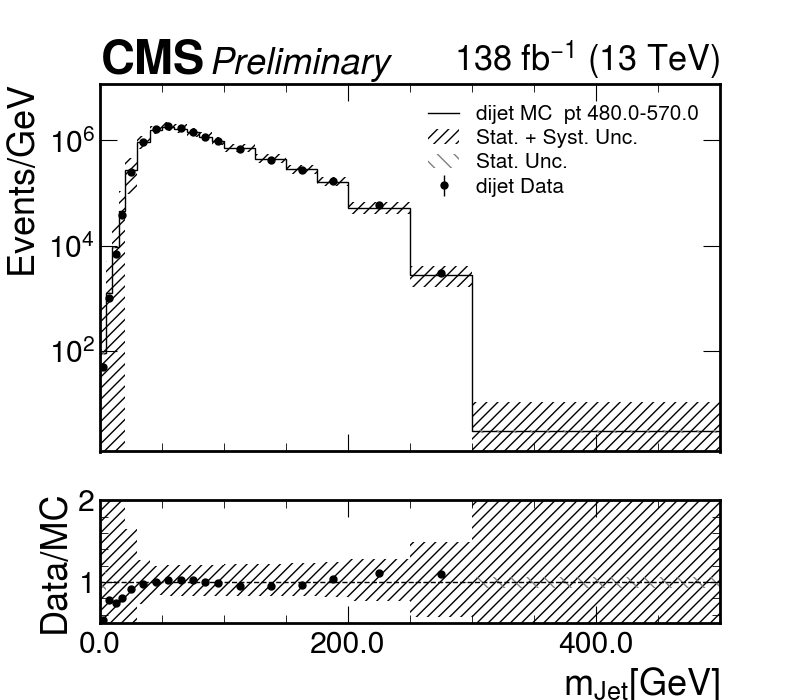
\includegraphics[width=0.45\textwidth]{figures/multijet/dijet/dijet_m_480_570.png}
  \end{subfigure}
  \begin{subfigure}
    \centering
    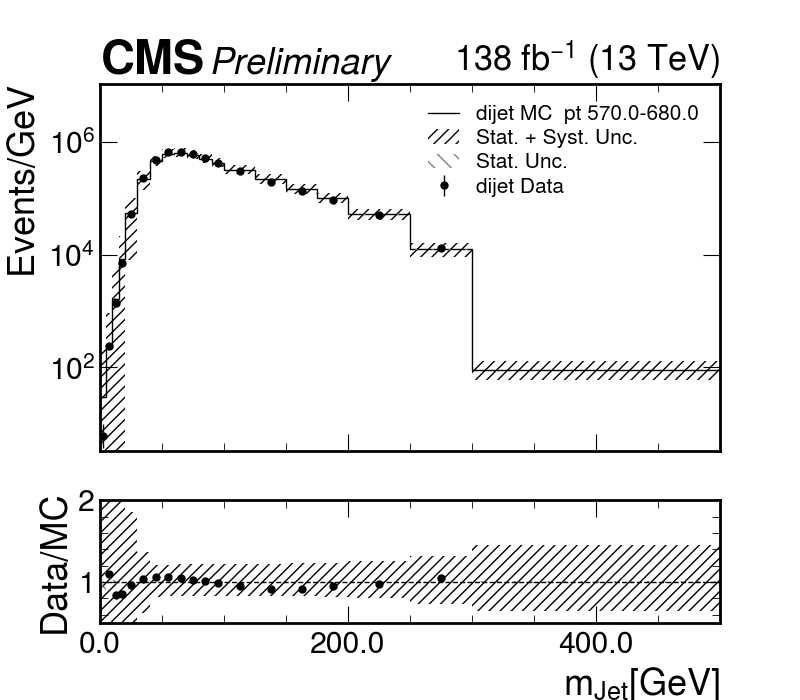
\includegraphics[width=0.45\textwidth]{figures/multijet/dijet/dijet_m_570_680.png}
  \end{subfigure}
  \begin{subfigure}
    \centering
    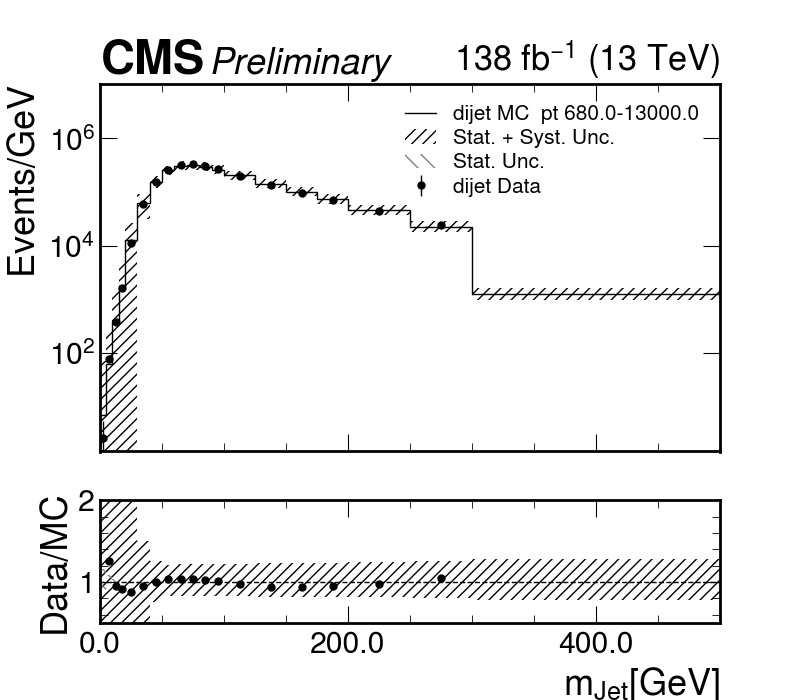
\includegraphics[width=0.45\textwidth]{figures/multijet/dijet/dijet_m_680_13000.png}
  \end{subfigure}
  \caption{Dijet channel  Data to MC comparison for ungroomed mass within each pT bin. MC is normalised to the integral of the data within each \pt bin.}
  \label{fig:17}
\end{figure}
\begin{figure}[h!]
  \centering
  \begin{subfigure}
    \centering
    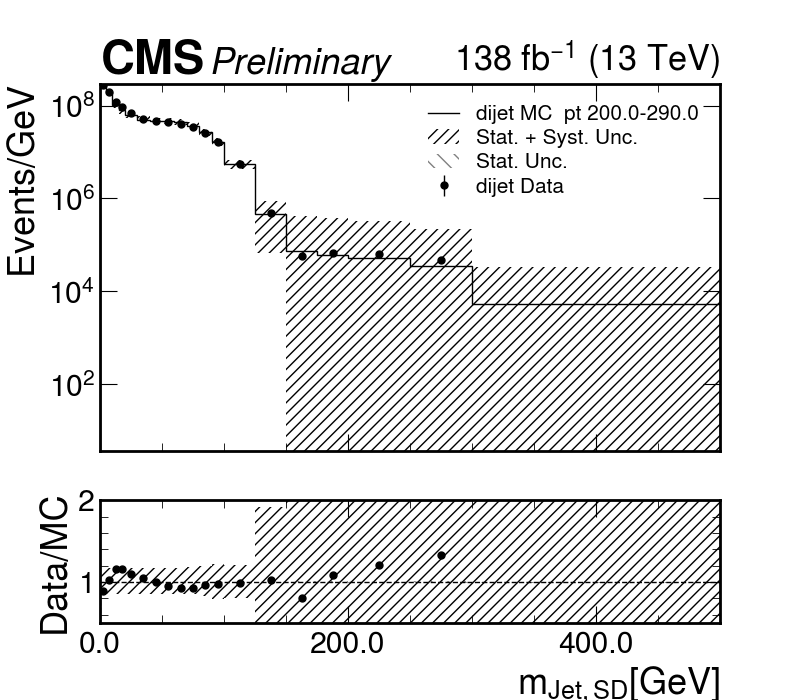
\includegraphics[width=0.45\textwidth]{figures/multijet/dijet/dijet_msd_200_290.png}
  \end{subfigure}
  \begin{subfigure}
    \centering
    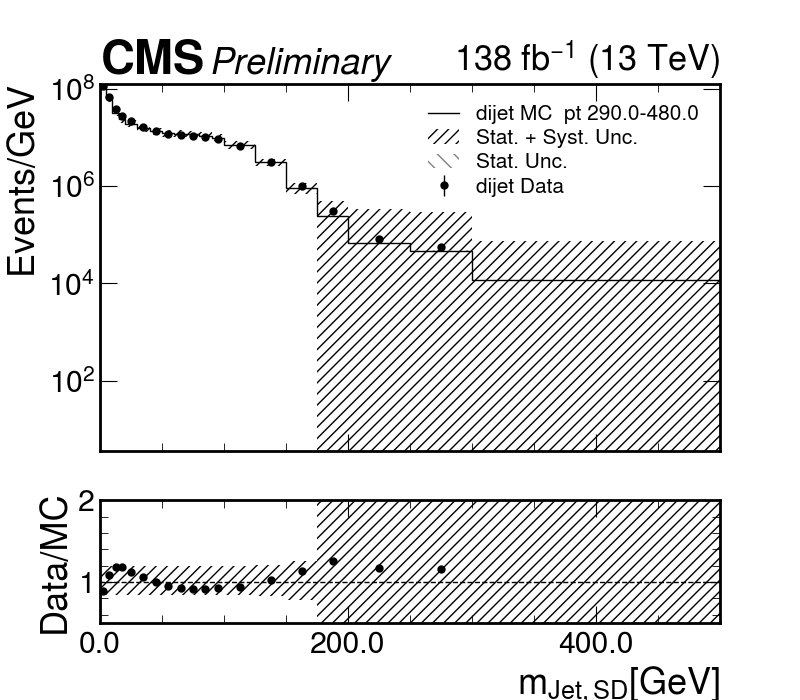
\includegraphics[width=0.45\textwidth]{figures/multijet/dijet/dijet_msd_290_480.png}
  \end{subfigure}
  \begin{subfigure}
    \centering
    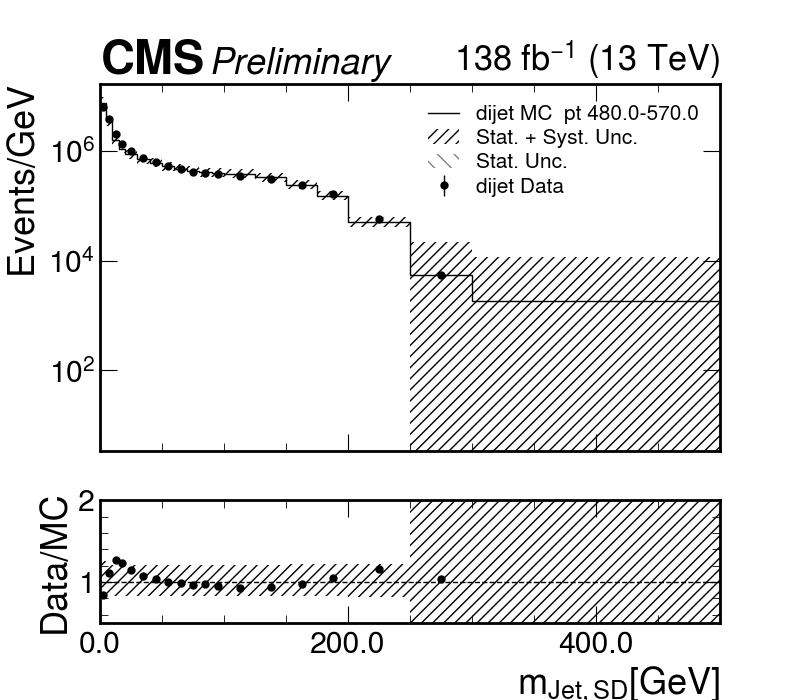
\includegraphics[width=0.45\textwidth]{figures/multijet/dijet/dijet_msd_480_570.png}
  \end{subfigure}
  \begin{subfigure}
    \centering
    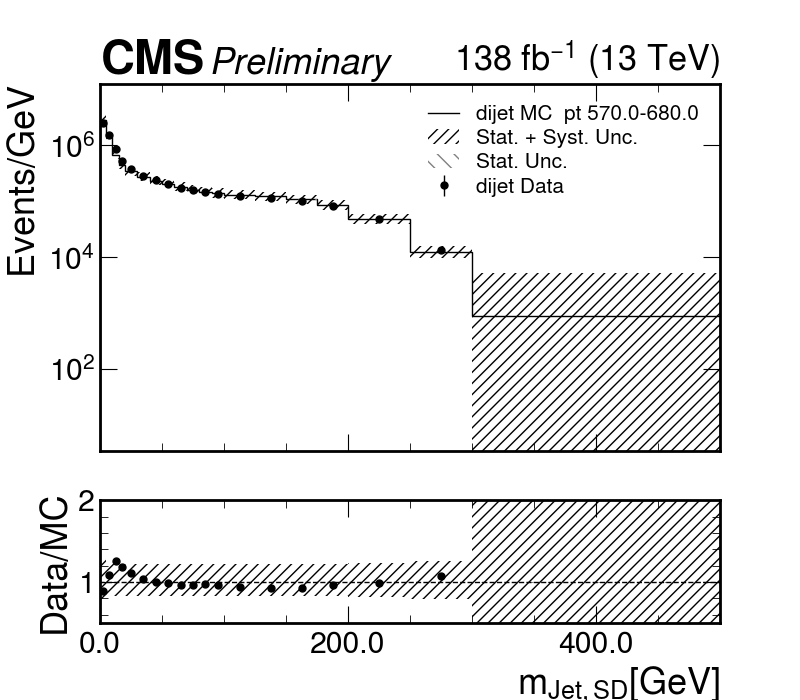
\includegraphics[width=0.45\textwidth]{figures/multijet/dijet/dijet_msd_570_680.png}
  \end{subfigure}
  \begin{subfigure}
    \centering
    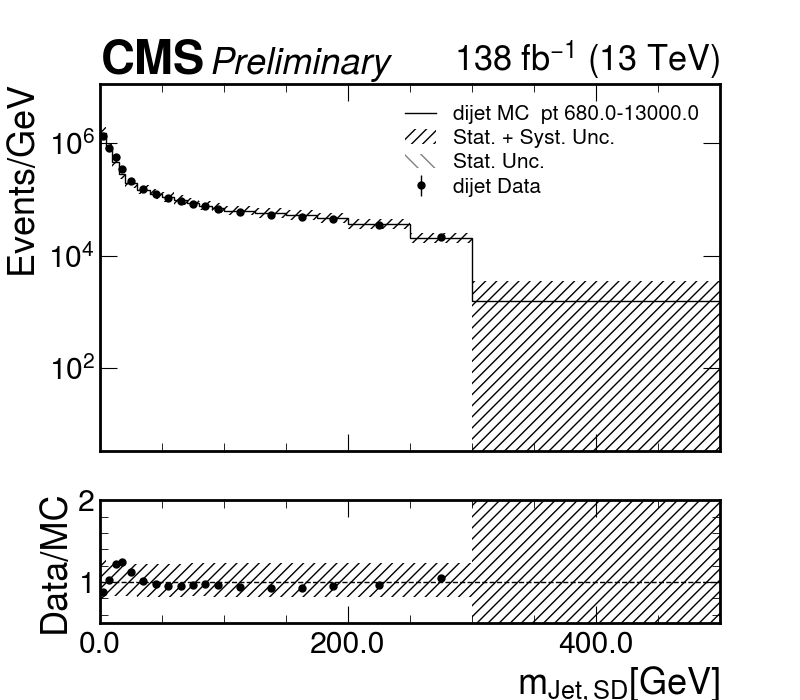
\includegraphics[width=0.45\textwidth]{figures/multijet/dijet/dijet_msd_680_13000.png}
  \end{subfigure}
  \caption{Dijet channel  Data to MC comparison for the softdrop mass within each pT bin. MC is normalised to the integral of the data within each \pt bin.}
  \label{fig:18}
\end{figure}

\begin{figure}[h!]
  \centering
  \begin{subfigure}
    \centering
    
    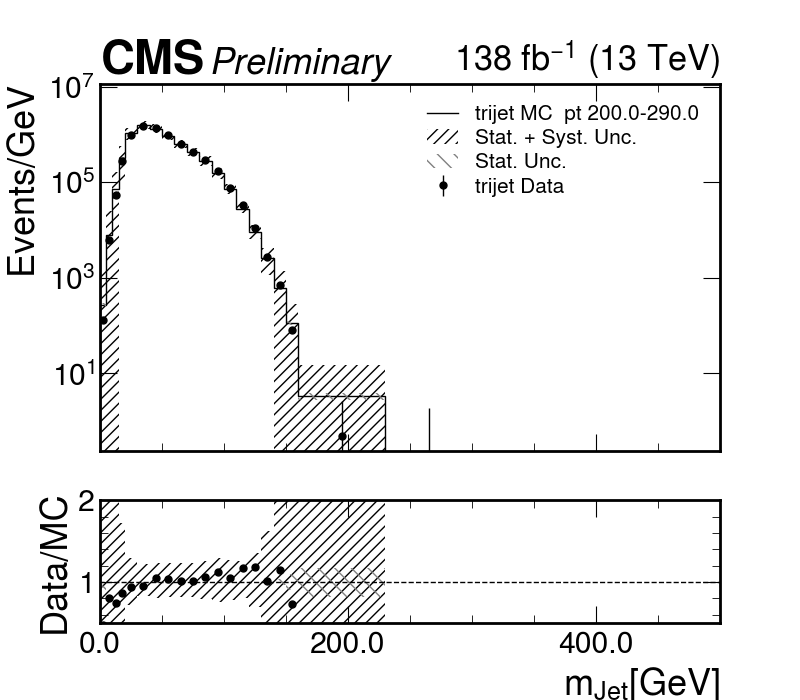
\includegraphics[width=0.45\textwidth]{figures/multijet/trijet/trijet_m_200_290.png}
  \end{subfigure}
  \begin{subfigure}
    \centering
    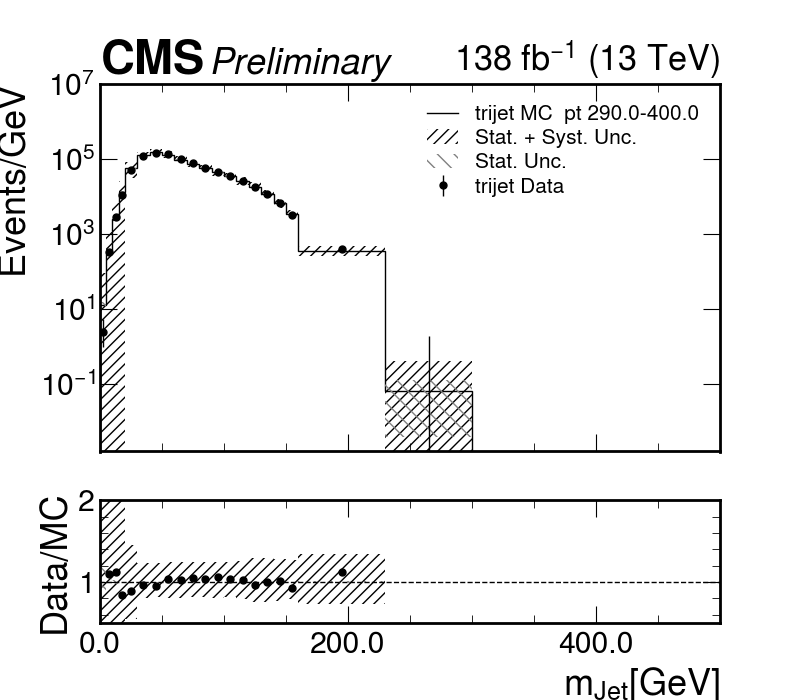
\includegraphics[width=0.45\textwidth]{figures/multijet/trijet/trijet_m_290_400.png}
  \end{subfigure}
  \begin{subfigure}
    \centering
    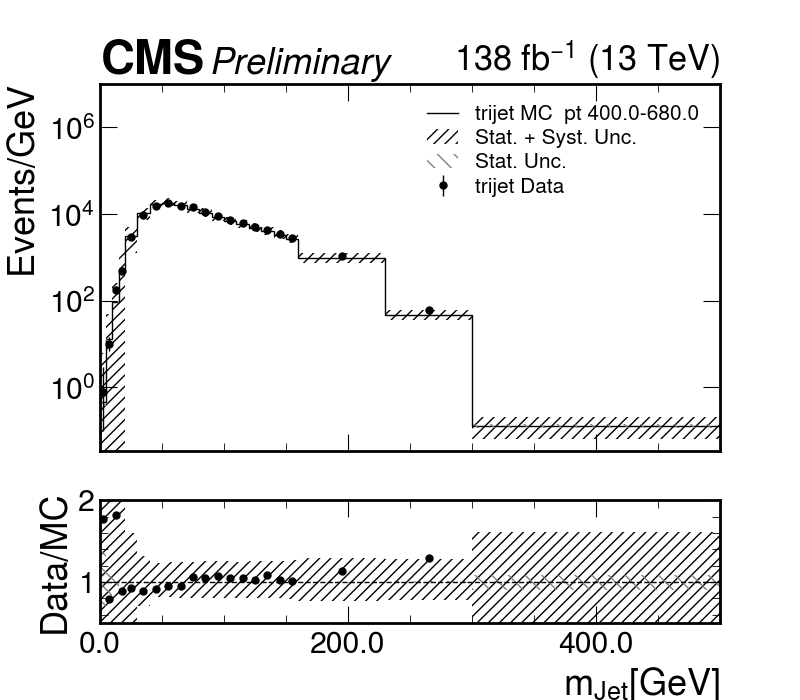
\includegraphics[width=0.45\textwidth]{figures/multijet/trijet/trijet_m_400_680.png}
  \end{subfigure}
  \begin{subfigure}
    \centering
    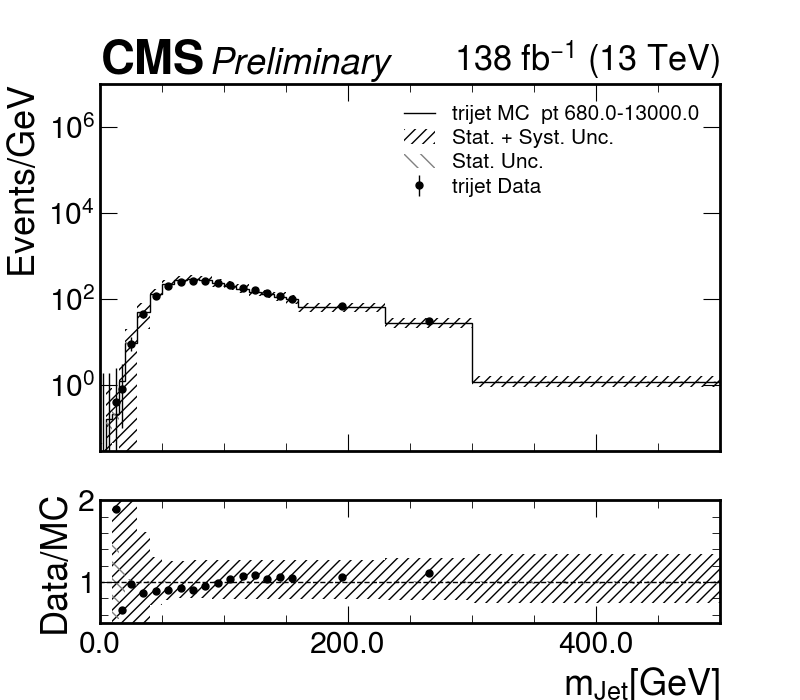
\includegraphics[width=0.45\textwidth]{figures/multijet/trijet/trijet_m_680_13000.png}
  \end{subfigure}
  \caption{Trijet channel  Data to MC comparison for ungroomed mass within each pT bin. MC is normalised to the integral of the data within each \pt bin.}
  \label{fig:19}
\end{figure}
\begin{figure}[h!]
  \centering
  \begin{subfigure}
    \centering
    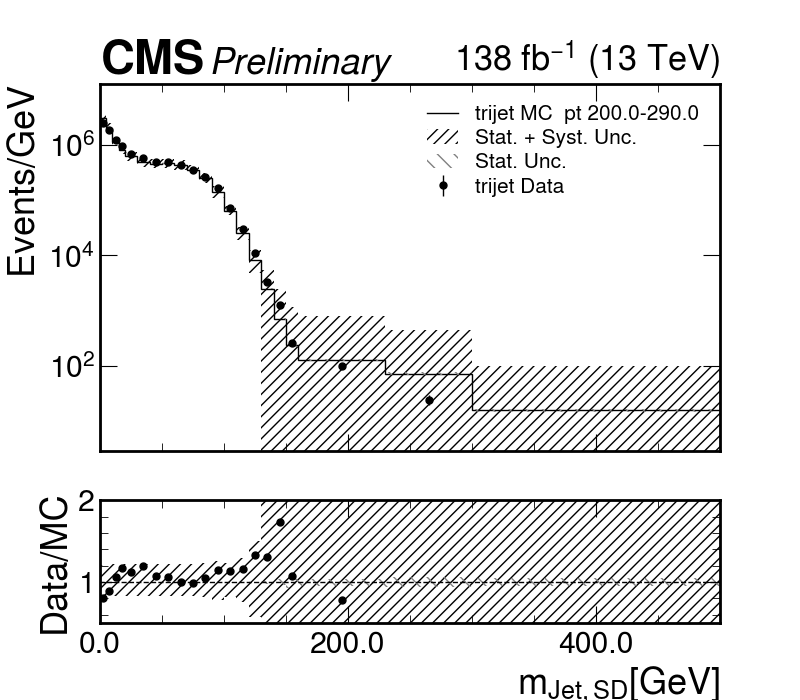
\includegraphics[width=0.45\textwidth]{figures/multijet/trijet/trijet_msd_200_290.png}
  \end{subfigure}
  \begin{subfigure}
    \centering
    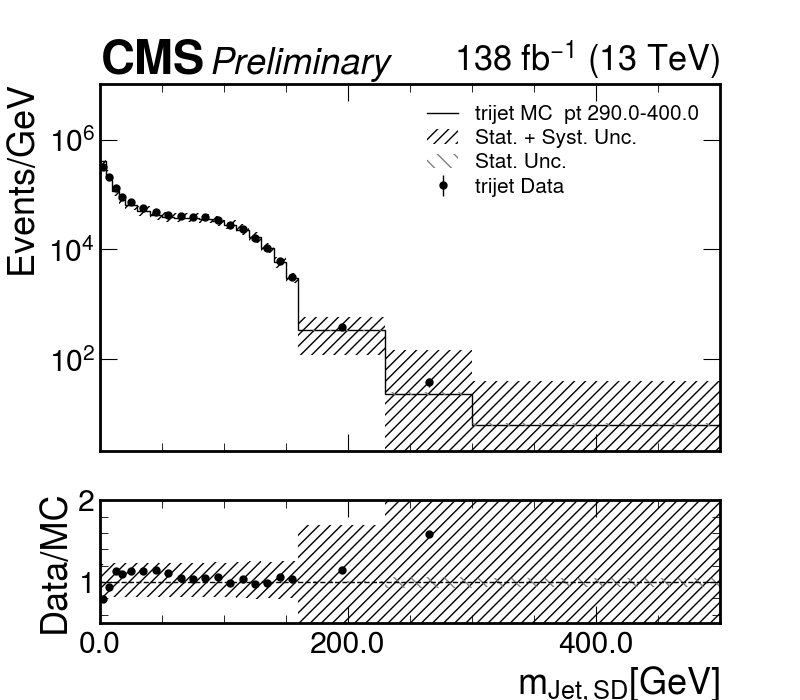
\includegraphics[width=0.45\textwidth]{figures/multijet/trijet/trijet_msd_290_400.png}
  \end{subfigure}
  \begin{subfigure}
    \centering
    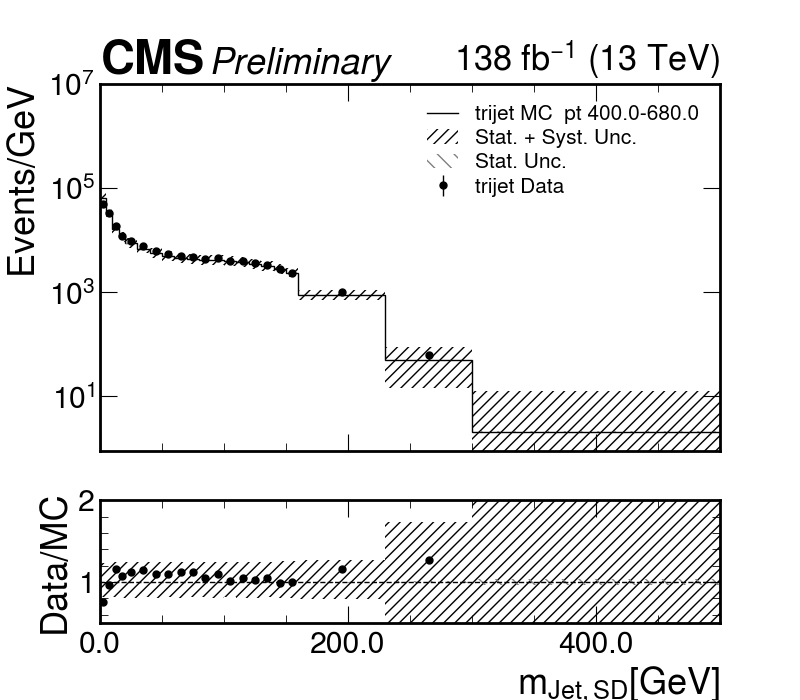
\includegraphics[width=0.45\textwidth]{figures/multijet/trijet/trijet_msd_400_680.png}
  \end{subfigure}
  \begin{subfigure}
    \centering
    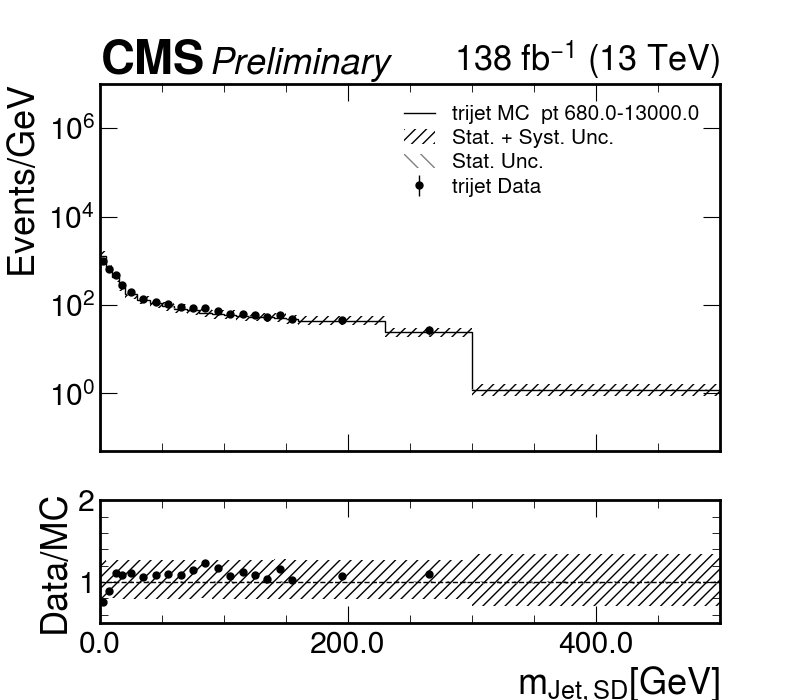
\includegraphics[width=0.45\textwidth]{figures/multijet/trijet/trijet_msd_680_13000.png}
  \end{subfigure}
  \caption{Trijet channel  Data to MC comparison for the softdrop mass within each pT bin. MC is normalised to the integral of the data within each \pt bin.}
  \label{fig:20}
\end{figure}


\section{Uncertainties}
The reconstructed events in this analysis are subject to statistical and systematic uncertainties that must be propagated through the unfolding to the final measurement.
\subsection{Statistical Uncertainty}
To estimate the statistical uncertainty after unfolding, the jackknife resampling method is employed \cite{economics_jk}. This method is helpful in estimating the variance of a limited sample set and is computed by finding the mean of $N$ independent subsamples of size $N-1$ of the dataset and weighting that by $\sqrt{N/N-1}$. In our case, this means producing N separate response matrices using a fraction $(N-1)/N$ of the data for each response matrix, leaving an independent $1/N-1$ fraction of events out of each matrix. The unfolded cross-section is computed for each of these response matrices and the final statisitical uncertainty for the total result is taken as
\begin{equation}
  \label{eq:jk}
  \sigma_{stat} = \sqrt{\frac{N}{N-1}}\sigma
\end{equation}
where $\sigma$ is the standard deviation of the N unfolded variations and $\sigma_{stat}$ is taken as the statistical uncertainty. In this analysis we used $N=10$ subsamples to compute the statistical uncertainty and the spread of these unfolded subsamples can be seen in figure \ref{fig:jk}.

\subsection{Systematic Uncertainties}
The sources of systematic uncertainties affecting this analysis are described in this section. Since the data is split into 4 distinct eras, the correlations of the uncertainties between the eras is also described.
\begin{itemize}
\item \textbf{Jet Energy Scale (JES)} Uncertainties associated with the JECs, as described in section \ref{JEC}, are derived by varying the scale by $\pm 1 \sigma$ for each individual uncertainty source. There are 27 uncertainty sources per year and their correlations between years are provided by the CMS collaboration \cite{JEC}. The correlation between years for each uncertainty source is shown in Table \ref{table:tab2}. For simplicity, given a correlation factor $\rho$ and a variation $\sigma$ , the correlated part $\sigma_{corr}$ and uncorrelated part of the variation $\sigma_{uncorr}$ are given by:
  \begin{equation}
    \label{eq:corr}
    \sigma_{corr}=\sigma\rho
  \end{equation}
    \begin{equation}
    \label{eq:uncorr}
    \sigma_{uncorr}=(1-\rho)\sigma
  \end{equation}
  Each uncertainty variation is considered in a separate response matrix and unfolded separately.
  \begin{table}[h!]
    \centering
    \begin{tabular}{lr}
      \hline
      Uncertainty & Correlation \\ \hline
      AbsoluteMPFBias & 100\% \\
      AbsoluteScale & 100\% \\
      AbsoluteStat & 0\% \\
      FlavorQCD & 100\% \\
      Fragmentation & 100\% \\
      PileUpDataMC & 50\% \\
      PileUpPtBB & 50\% \\
      PileUpPtEC1 &50\% \\
      PileUpPtEC2 & 50\% \\
      PileUpPtHF & 50\% \\
      PileUpPtRef & 50\% \\
      RelativeFSR & 50\% \\
      RelativeJEREC1 & 0\% \\
      RelativeJEREC2 & 0\% \\
      RelativeJERHF & 50\% \\
      RelativePtBB & 50\% \\
      RelativePtEC1 & 0\% \\
      RelativePtEC2 & 0\% \\
      RelativePtHF & 50\% \\
      RelativeBal & 50\% \\
      RelativeSample & 0\% \\
      RelativeStatEC & 0\% \\
      RelativeStatFSR & 0\% \\
      RelativeStatHF & 0\% \\
      SinglePionECAL & 100\% \\
      SinglePionHCAL & 100\% \\
      TimePtEta & 0\% \\ \hline
    \end{tabular}
    \caption{Correlations between data taking periods for all JEC uncertainty sources.}
    \label{table:tab2}
  \end{table}
\item \textbf{Jet Energy Resolution (JER):} Similar to the JES uncertainties, the JER uncertainty is a $1\sigma$ shift and fully correlated in  \pt and $\eta$ and uncorrelated across years. Again, these uncertainty values are provided by the CMS Collaboartion \cite{JEC}.
\item \textbf{Jet Mass Scale (JMS) and Resolution (JMR)} Just like the JES and JER uncertainties, the JMS and JMR uncertainties are calculated as a 1 sigma shift (?). These values are again provided by the collaboration and can be seen in the \ref{table:JMS}.
\item \textbf{Integrated Luminosity:}
 The uncertainty on the measurement of the full Run II luminosity$\script{L}_{int}\approx 137.2 fb^{-1}$ is estimated to be 1.6\% \cite{lumi2016, lumi2017, lumi2018}. This uncertainty is accounted for as its own response matrix and normalized post unfolding.
\item \textbf{Pileup Re-weighting:}
 As decribed in \ref{PUSF}, simulation samples are reweighted to match the pileup profile in data from the using the number of interactions per bunch crossing. This is estimated from measurements of the luminosity and the inclusive cross section for Run II $\sigma^{inel}_{pp} = 69.2 mb$ \cite{LUMIPOGtwiki}. The corresponding uncertainty is calculated by varying the total inelastic cross section by $\pm 4.6\%$ and repeating the reweighting. The uncertainties are treated as fully correlated between data taking eras.
\item \textbf{Parton Distribution Functions (PDFs):}
  The simulated samples contain per-event weights for 100 variations of the original NNPDF3.1 PDF set \cite{nnpdf3.1}. The corresponding systematic uncertainty is taken as the RMS deviation of the variations.
\item \textbf{$q^2$ Scales:}
  The simulated samples contain weights that correspond to variations in the in the factorisation, $\mu_F$ and renormalisation $\mu_R$ scales. The scales are each varied separately by factors of 0.5 and 2 separately, giving 9 permutations in total. Three of these cases are not considered since they vary the scales in the opposite direction, which is unphysical. The other 6 variations (both varied by 2, both varied by 0.5, $\mu_f$ varied up while $\mu_R$ is nominal and vice versa, and  $\mu_f$ varied down while $\mu_R$ is nominal and vice versa) are used to calculate the total scale uncertainty using the envelope method, where the largest observed deviation from the nominal $q^2$ setting is taken as the systematic uncertainty.
\item \textbf{L1 Prefiring:}
  As described in section \ref{prefiring}, during 2016 and 2017 data-taking, there was an additional inefficiency due to an issue in the L1 prefiring. This is corrected for using weights provided by the collaboration. The uncertainties are also provided by the collaboration, and are calculated by shifting the prefiring probabilities by the squared sum of $20\%$ of the prefiring probability and the statistical uncertatinty in each considered bin used to make the pefiring map \cite{l1prefiring}.
\item \textbf{Parton Shower and Hadronization Model}
  We use a separate MG+HERWIG sample to model the effects of the parton shower and hadronisation model. We create a separate response matrix using this model just as we do with each other uncertainty mentioned, unfold the data using it, and include it as an uncertainty. The difference between the herwig and pythia distributions can be seen in figure \ref{fig:herwig}. The resulting uncertainty after unfolding can be seen in the plots in the right column of figures \ref{fig:dijetunc} and \ref{fig:trijetunc}.
  % \item \textbf{HEM} --> not needed if we're veto-ing HEM events
  All of the above uncertainties can be be seen before unfolding and for the ungroomed mass for the dijet(trijet) channel in figure \ref{fig:dijetunc_ungroomed}(\ref{fig:trijetunc_ungroomed}, beforand after unfolding for the ungroomed mass in the dijet(trijet) channel in figure \ref{fig:dijetunc_ungroomed_postunfold}(\ref{fig:trijetunc_ungroomed_postunfold}). For the groomed mass, the uncertainties before unfolding in the dijet(trijet) channel can be seen in figure \ref{fig:dijetunc_groomed}(\ref{fig:trijetunc_groomed}), and after unfolding in figure \ref{fig:dijetunc_groomed_postunfold}(\ref{fig:trijetunc_groomed_postunfold}).
\end{itemize}
\begin{figure}[ht!]
  \centering
  \begin{subfigure}
    \centering
    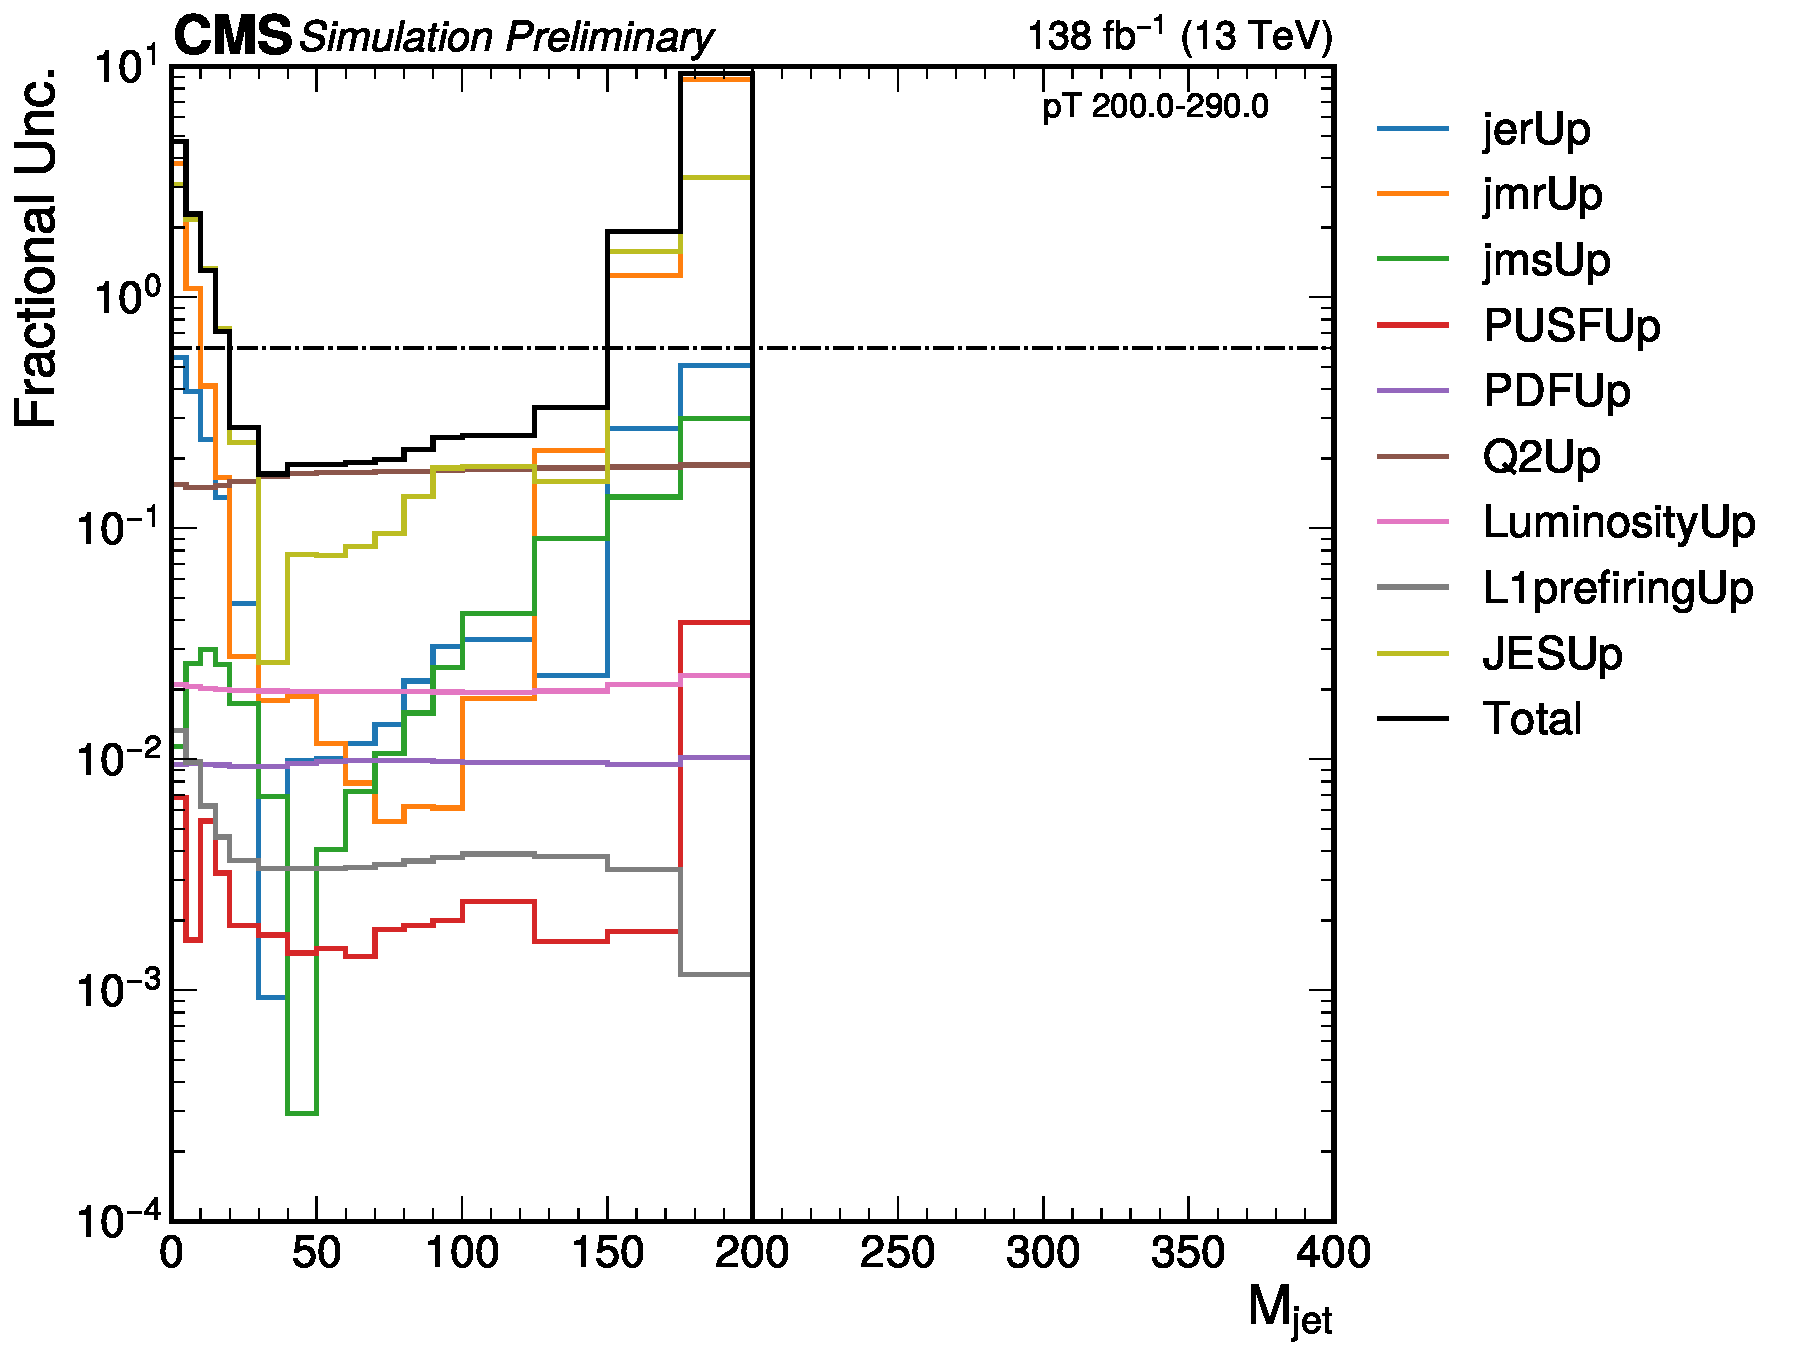
\includegraphics[width=0.45\textwidth]{figures/multijet/dijet/fracUnc_ungroomed_0.pdf}
\end{subfigure} 
  \begin{subfigure}
    \centering
    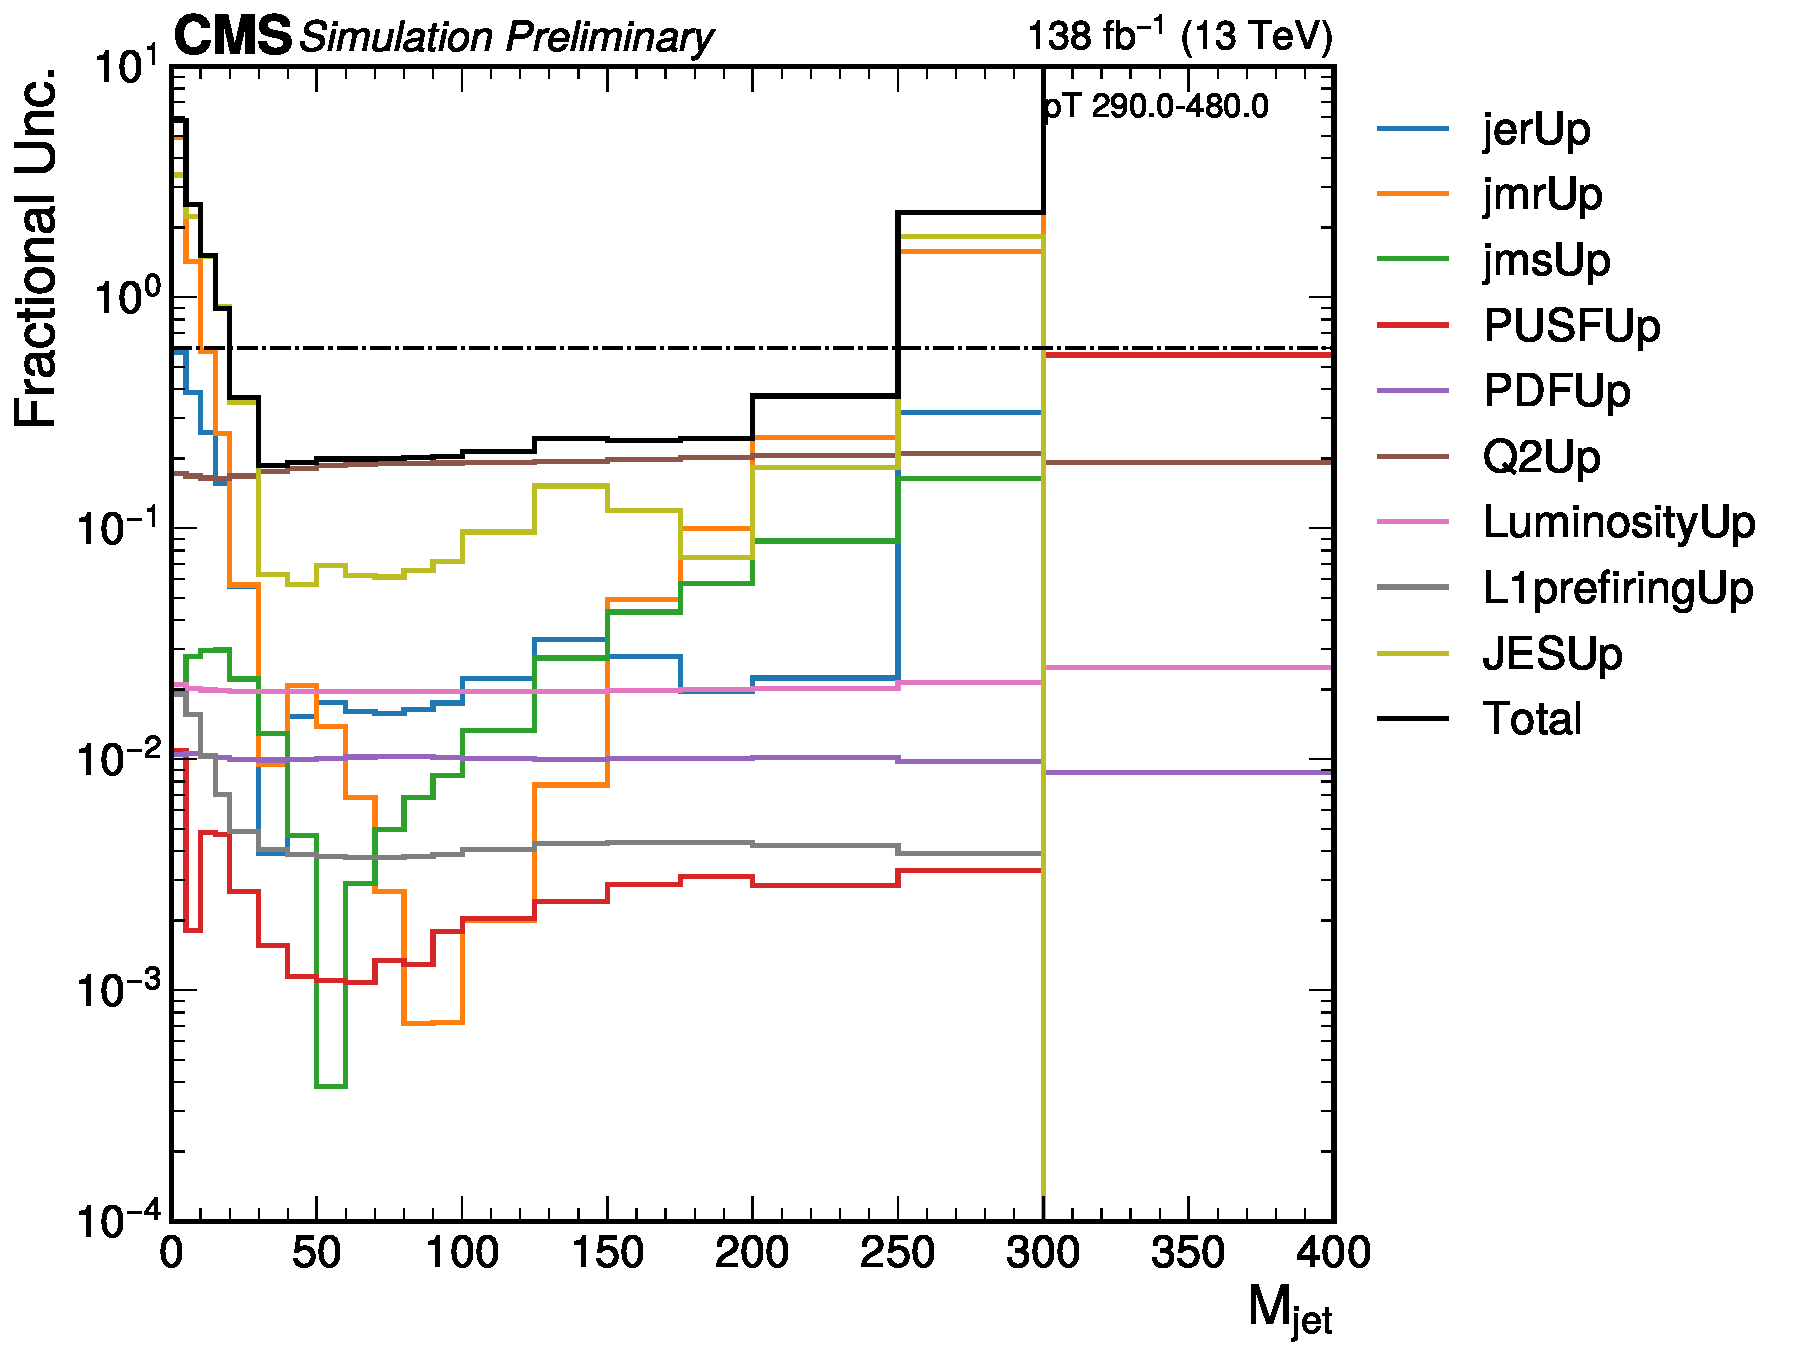
\includegraphics[width=0.45\textwidth]{figures/multijet/dijet/fracUnc_ungroomed_1.pdf}
\end{subfigure}
  \begin{subfigure}
    \centering
    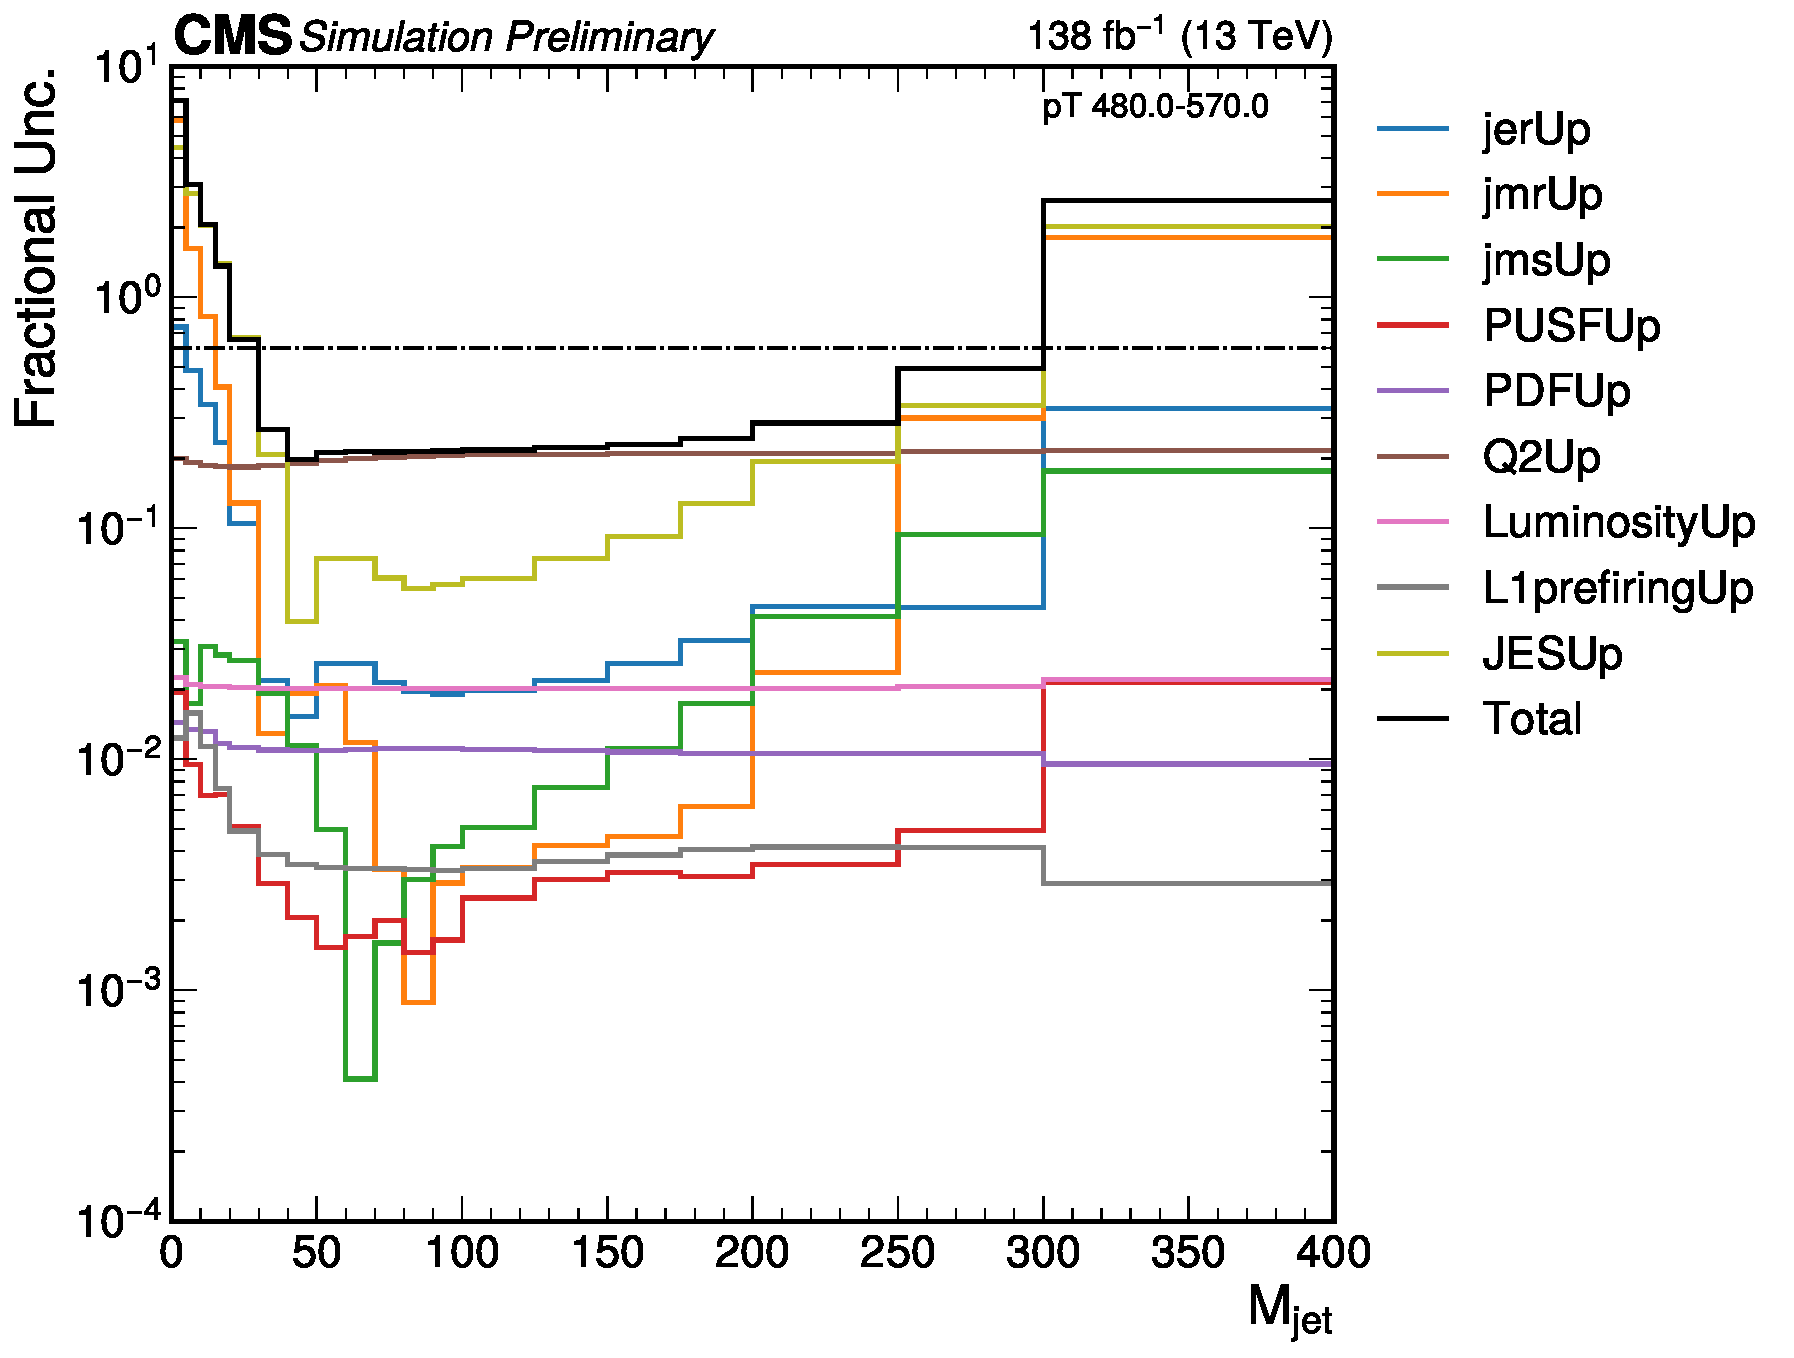
\includegraphics[width=0.45\textwidth]{figures/multijet/dijet/fracUnc_ungroomed_2.pdf}
\end{subfigure}
  \begin{subfigure}
    \centering
    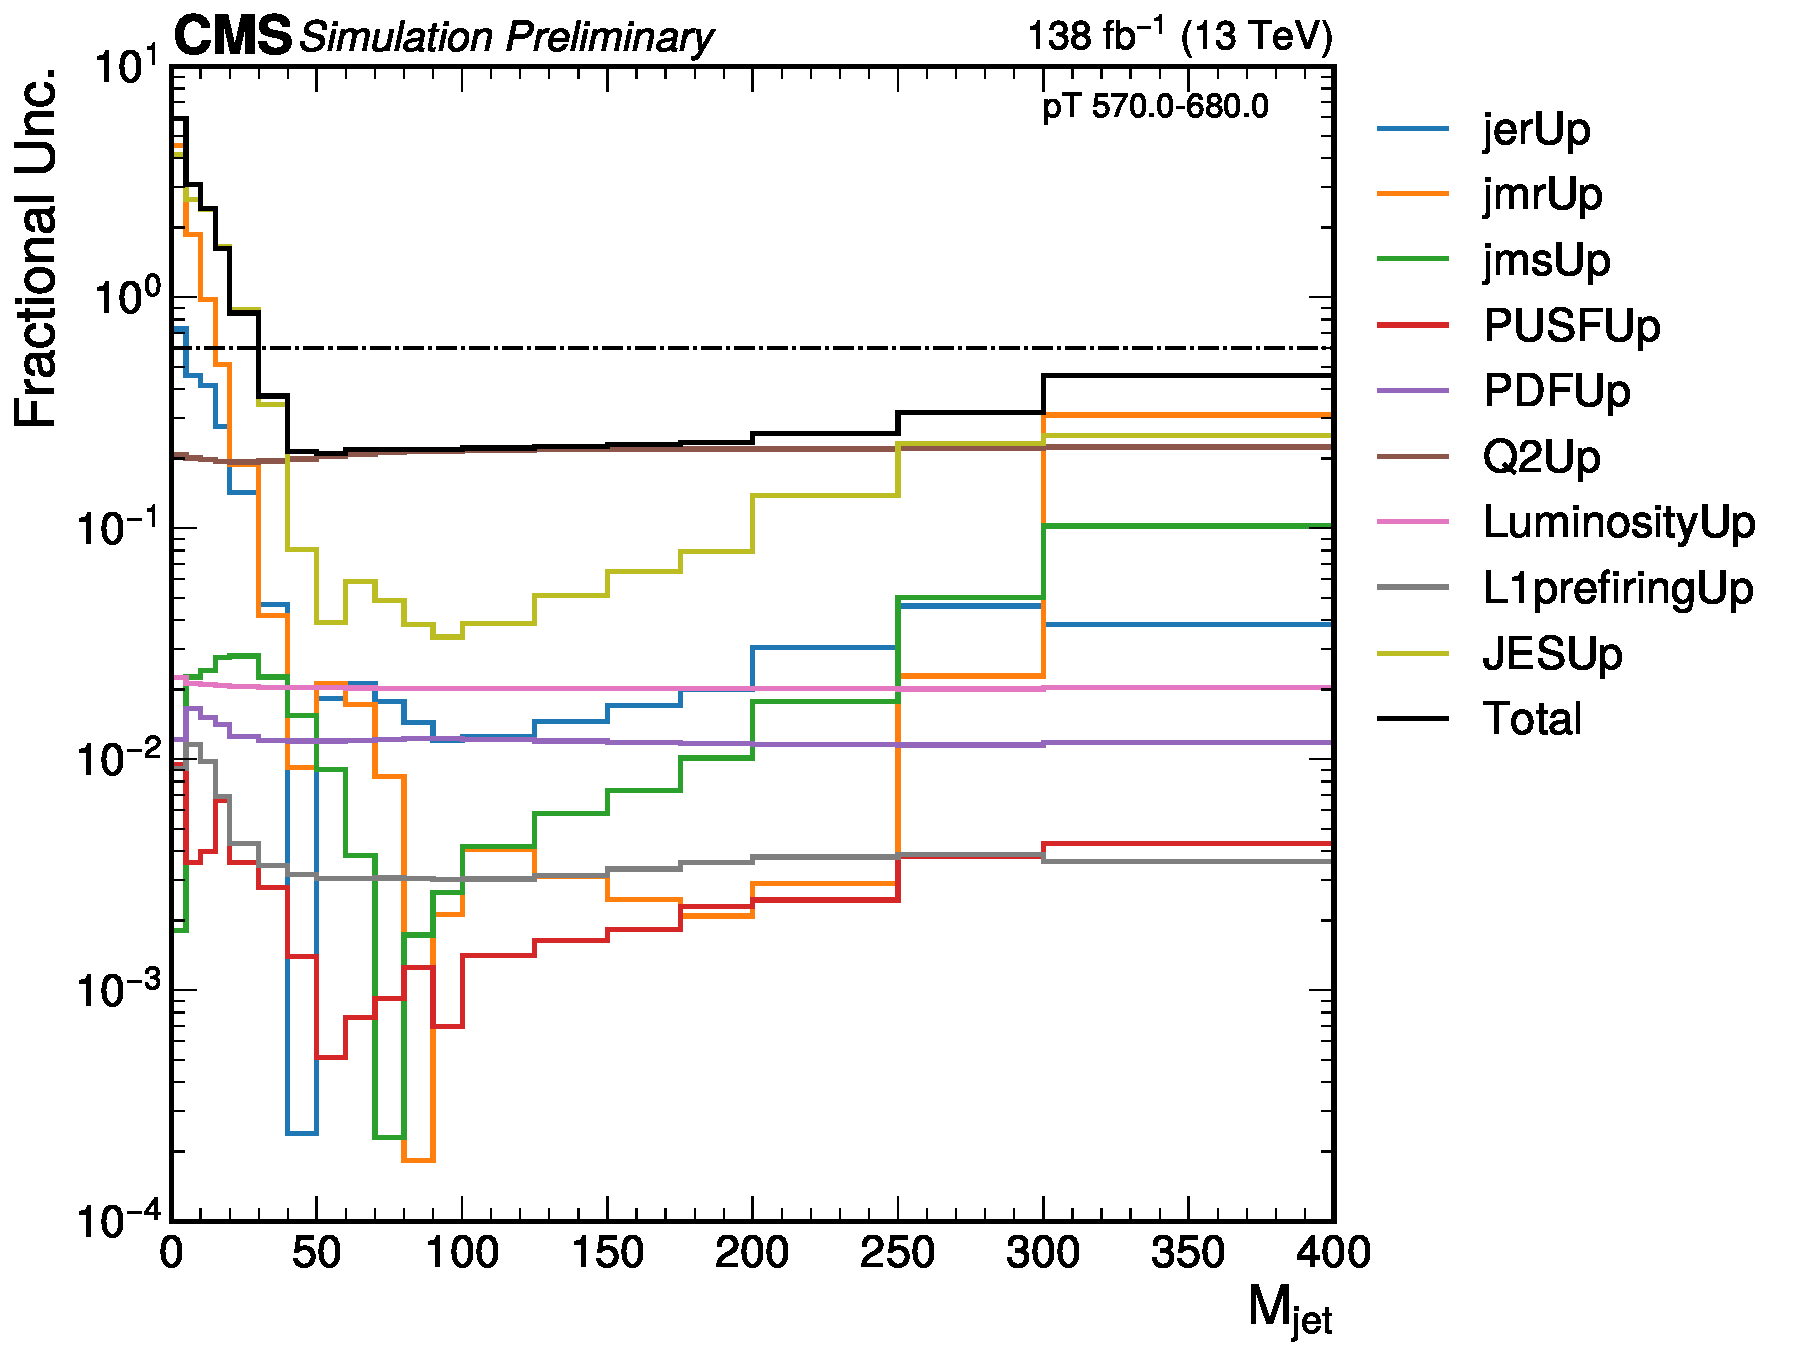
\includegraphics[width=0.45\textwidth]{figures/multijet/dijet/fracUnc_ungroomed_3.pdf}
\end{subfigure}
  \begin{subfigure}
    \centering
    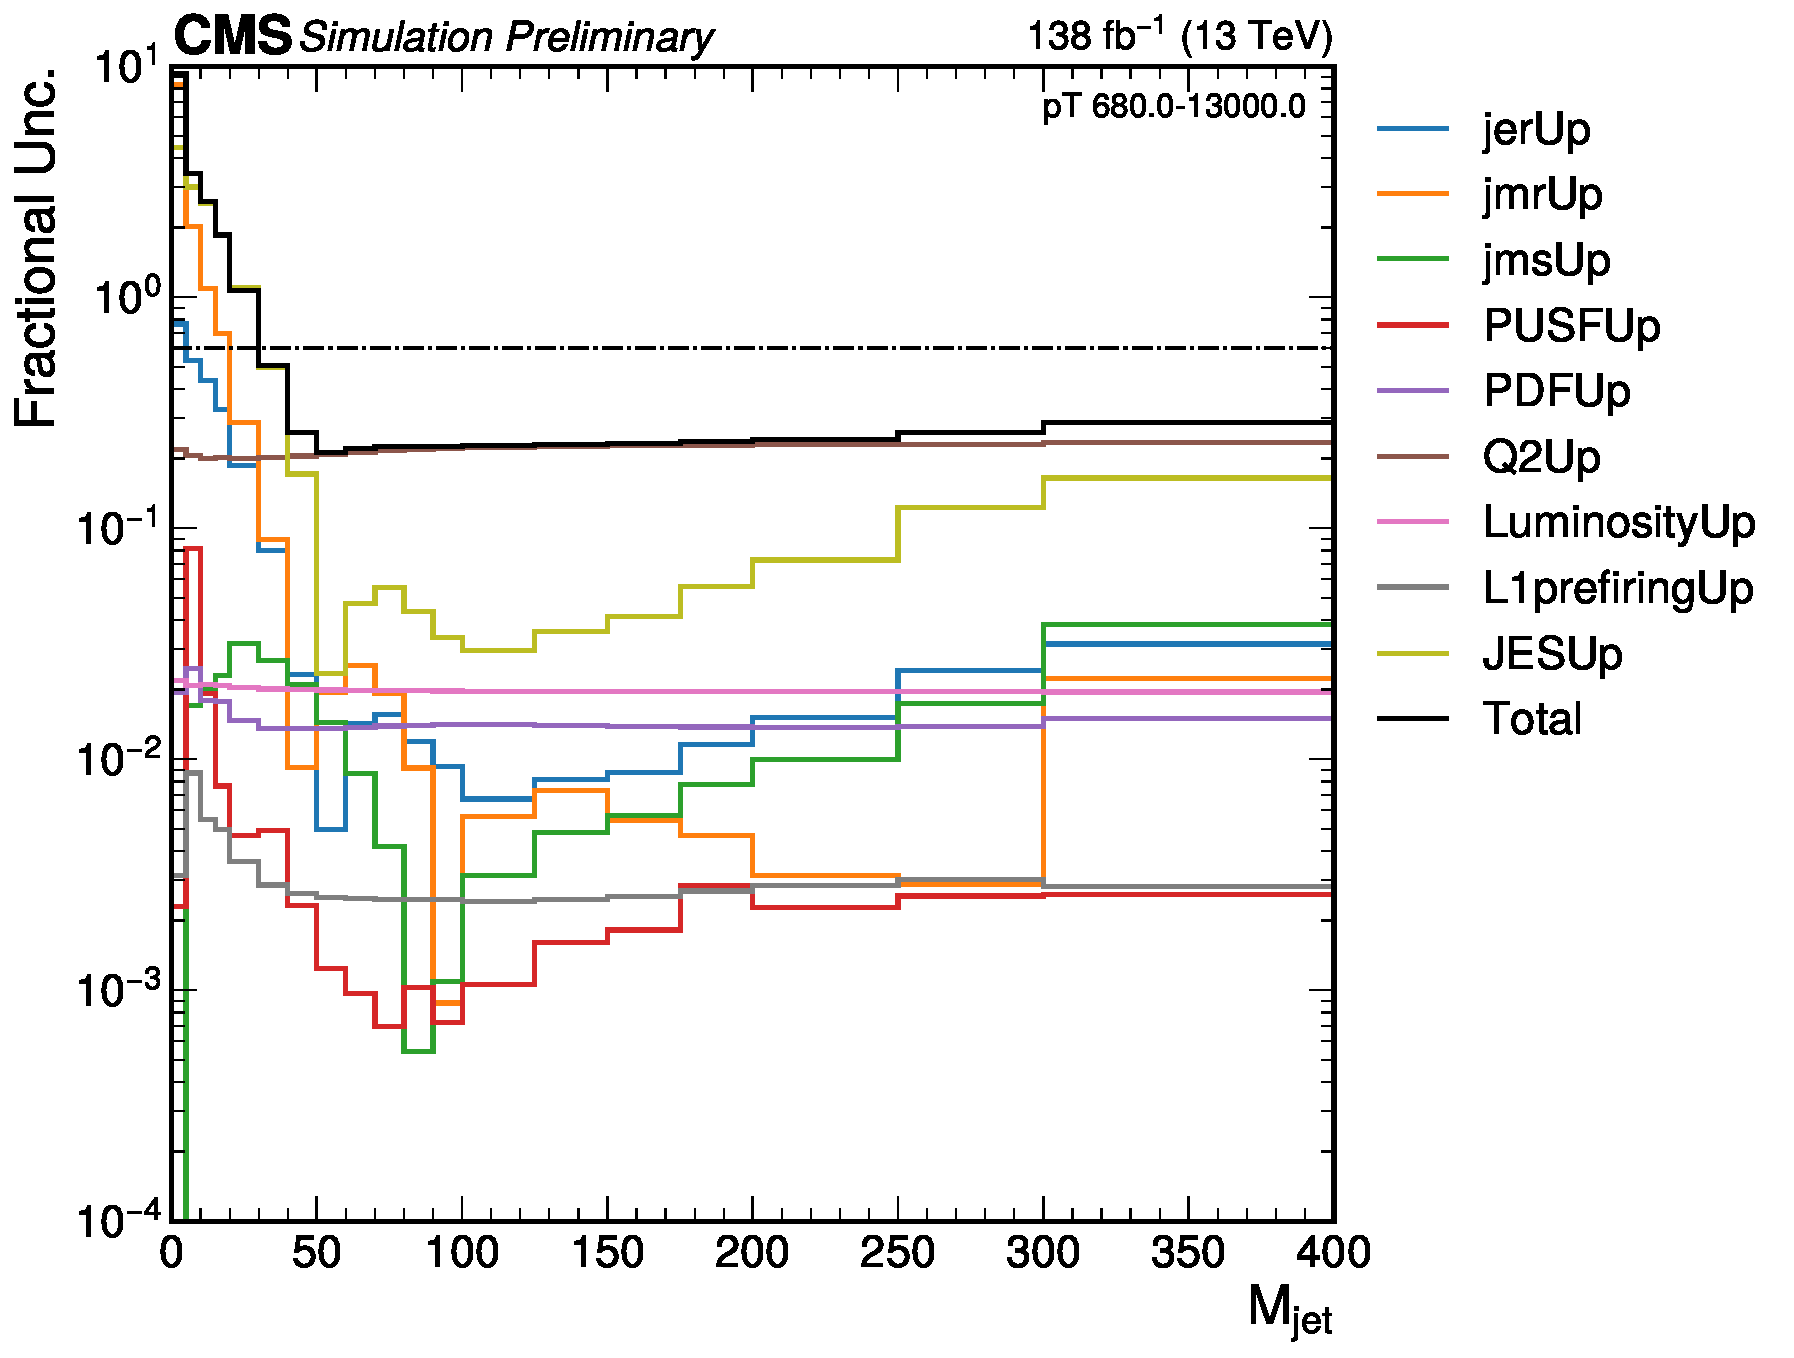
\includegraphics[width=0.45\textwidth]{figures/multijet/dijet/fracUnc_ungroomed_4.pdf}
\end{subfigure}
  \caption{Uncertainties per bin before unfolding in the ungroomed dijet channel.}
  \label{fig:dijetunc_ungroomed}
  \end{figure}
\begin{figure}[ht!]
  \centering
  \begin{subfigure}
    \centering
    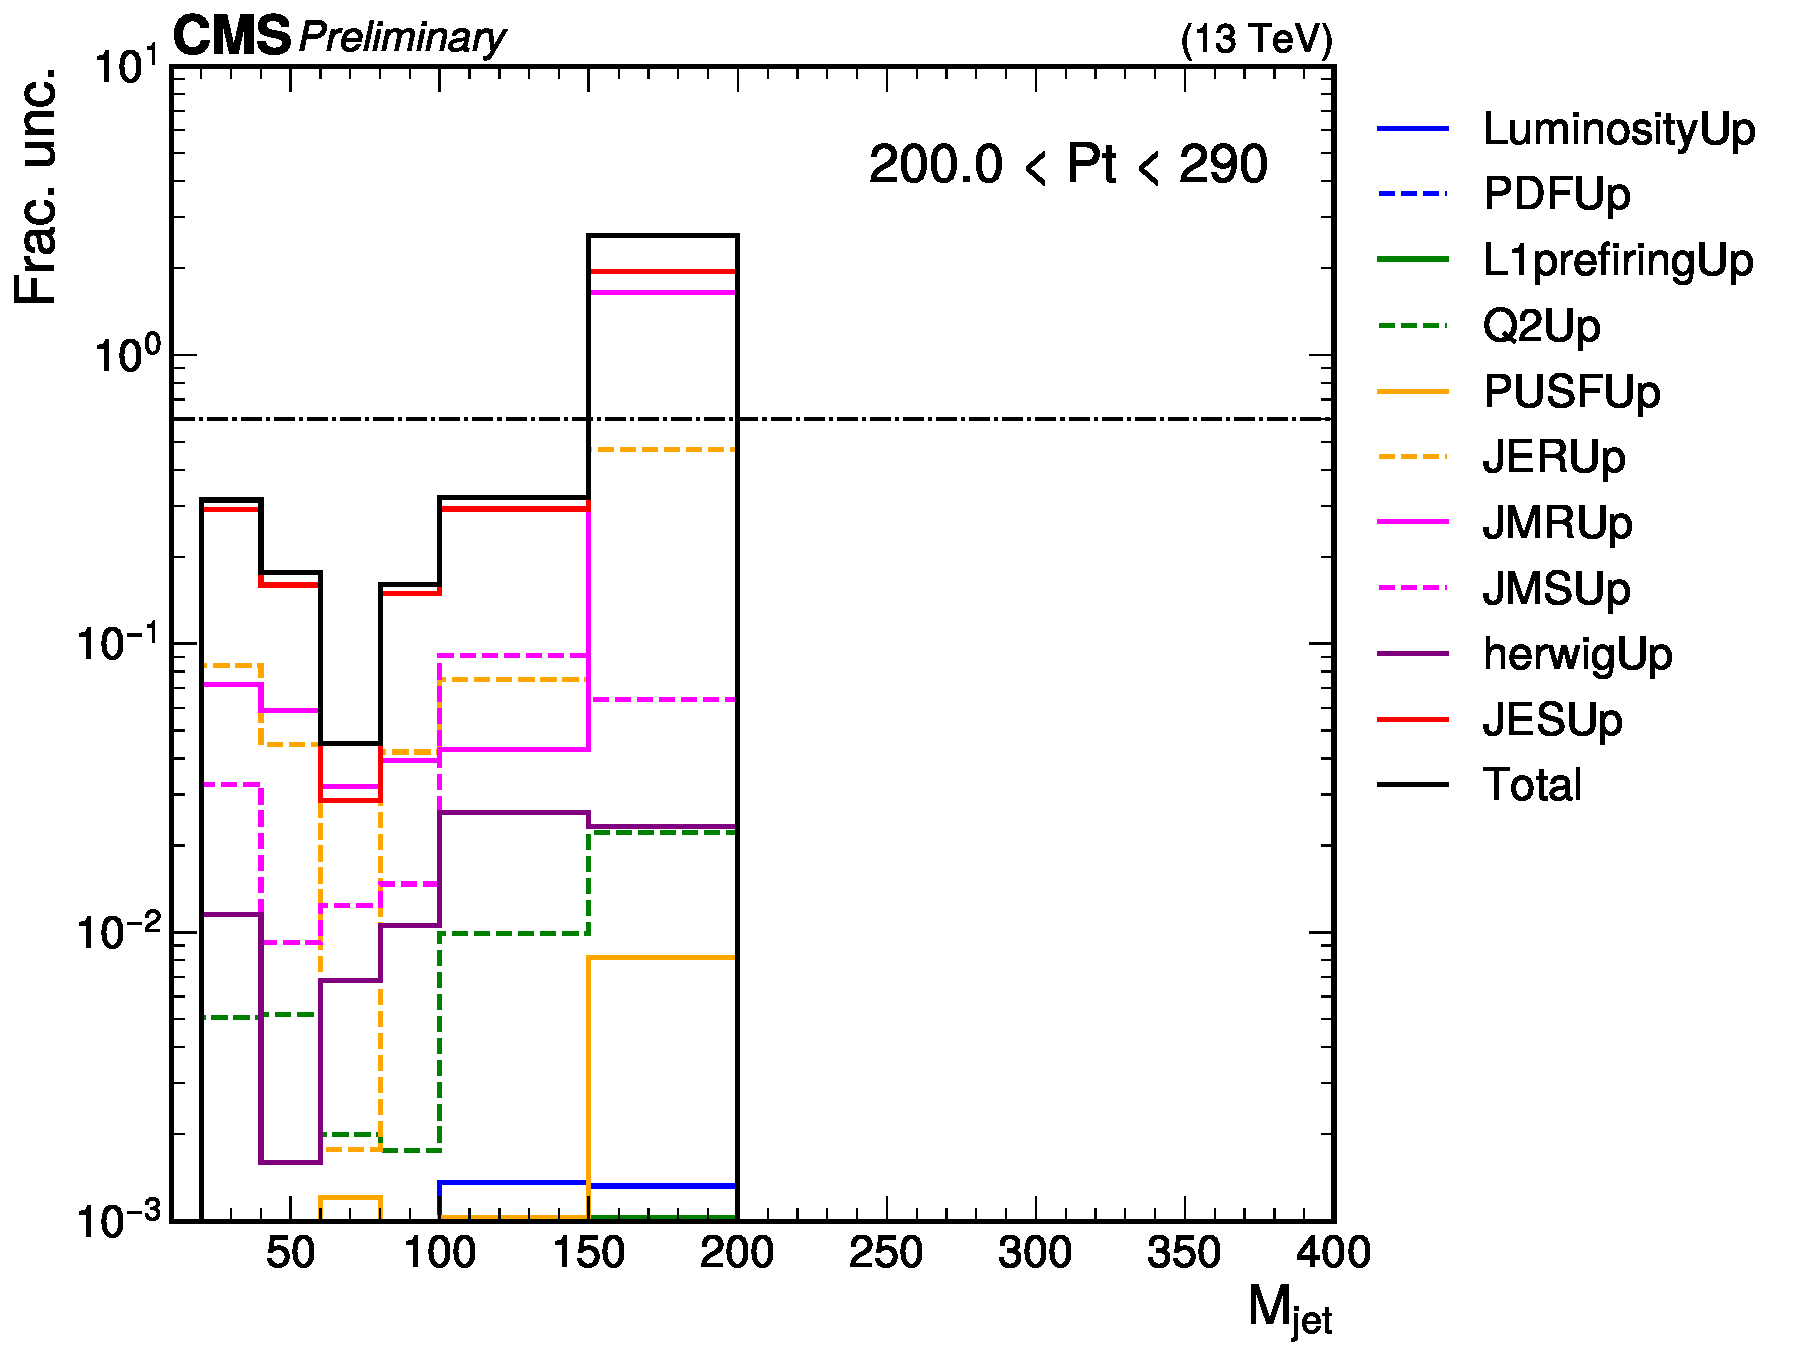
\includegraphics[width=0.45\textwidth]{figures/multijet/unfolding/dijet/unfolded_fracUnc_ungroomed_0.pdf}
\end{subfigure}
  \begin{subfigure}
    \centering
    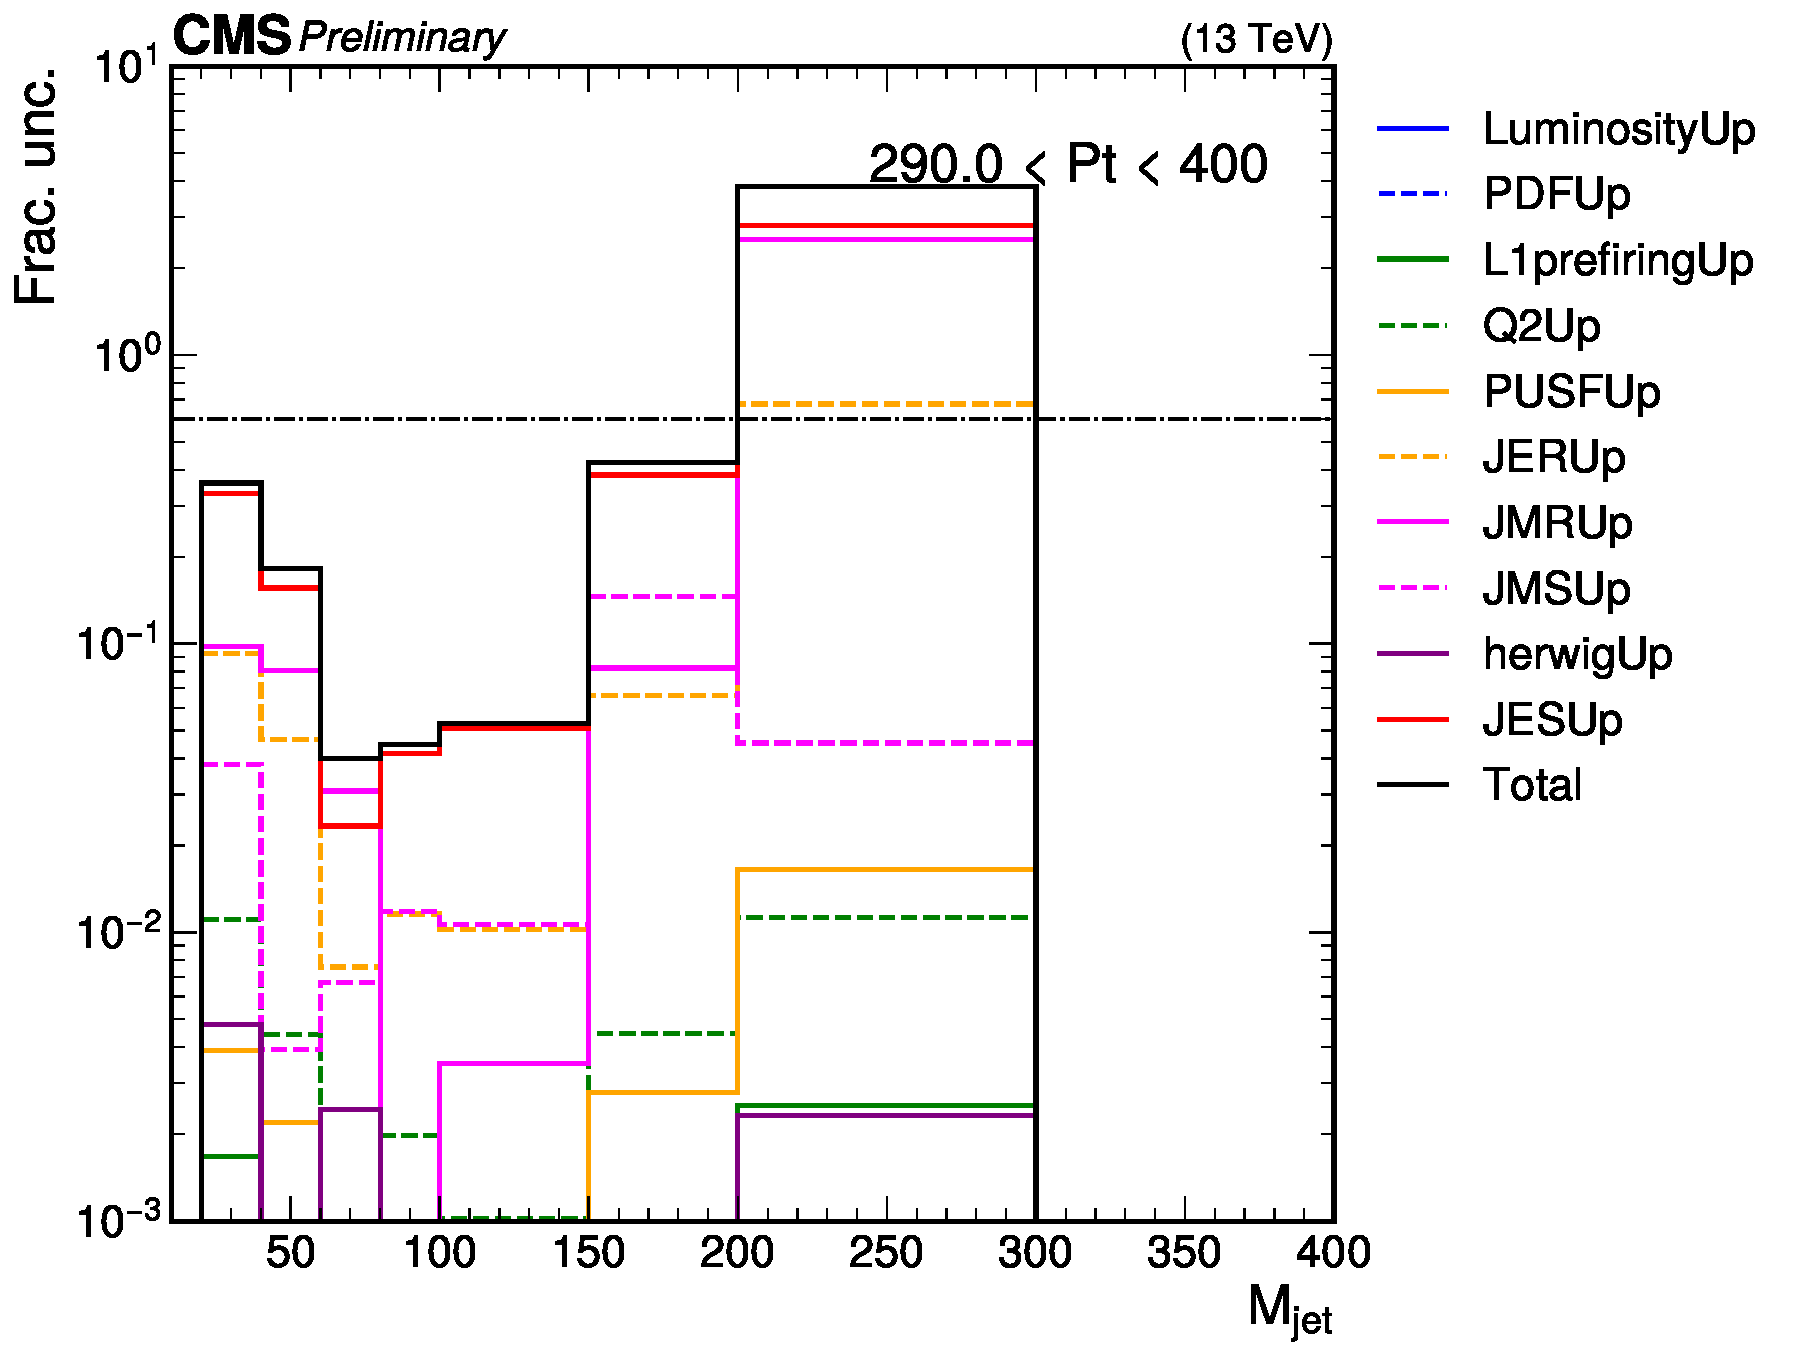
\includegraphics[width=0.45\textwidth]{figures/multijet/unfolding/dijet/unfolded_fracUnc_ungroomed_1.pdf}
\end{subfigure}
  \begin{subfigure}
    \centering
    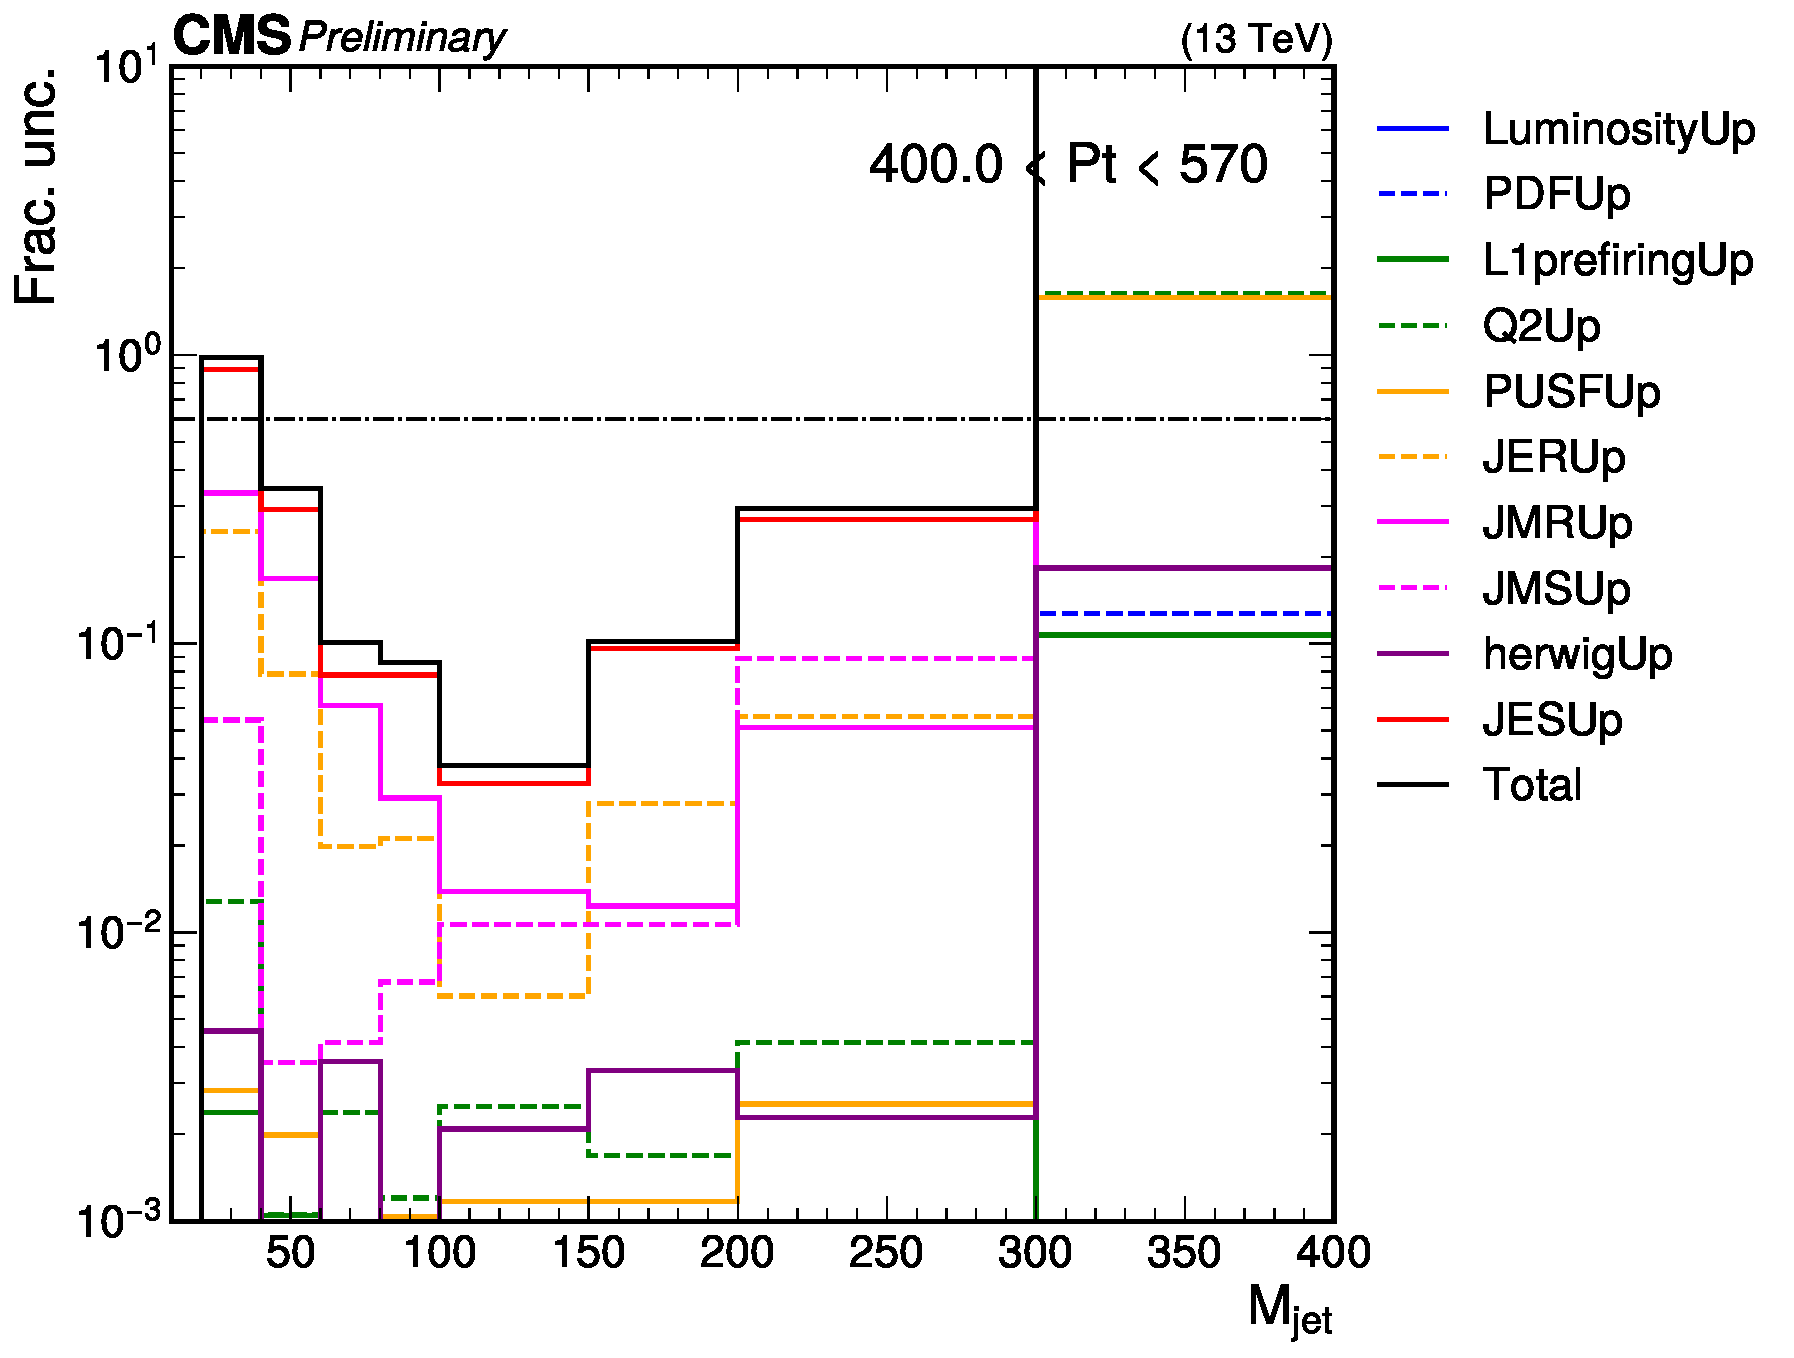
\includegraphics[width=0.45\textwidth]{figures/multijet/unfolding/dijet/unfolded_fracUnc_ungroomed_2.pdf}
\end{subfigure}
\begin{subfigure}
    \centering
    \includegraphics[width=0.45\textwidth]{figures/multijet/unfolding/dijet/unfolded_fracUnc_ungroomed_3.pdf}
\end{subfigure}
  \begin{subfigure}
    \centering
    \includegraphics[width=0.45\textwidth]{figures/multijet/unfolding/dijet/unfolded_fracUnc_ungroomed_4.pdf}
\end{subfigure}
  \caption{Uncertainties per bin and after unfolding in the ungroomed dijet channel.}
  \label{fig:dijetunc_ungroomed_postunfold}
\end{figure}
\begin{figure}[ht!]
  \centering
  \begin{subfigure}
    \centering
    \includegraphics[width=0.45\textwidth]{figures/multijet/dijet/fracUnc_groomed_0.pdf}
\end{subfigure} 
  \begin{subfigure}
    \centering
    \includegraphics[width=0.45\textwidth]{figures/multijet/dijet/fracUnc_groomed_1.pdf}
\end{subfigure}
  \begin{subfigure}
    \centering
    \includegraphics[width=0.45\textwidth]{figures/multijet/dijet/fracUnc_groomed_2.pdf}
\end{subfigure}
  \begin{subfigure}
    \centering
    \includegraphics[width=0.45\textwidth]{figures/multijet/dijet/fracUnc_groomed_3.pdf}
\end{subfigure}
  \begin{subfigure}
    \centering
    \includegraphics[width=0.45\textwidth]{figures/multijet/dijet/fracUnc_groomed_4.pdf}
\end{subfigure}
  \caption{Uncertainties per bin before unfolding in the groomed dijet channel.}
  \label{fig:dijetunc_groomed}
  \end{figure}
\begin{figure}[ht!]
  \centering
  \begin{subfigure}
    \centering
    \includegraphics[width=0.45\textwidth]{figures/multijet/unfolding/dijet/unfolded_fracUnc_groomed_0.png}
\end{subfigure}
  \begin{subfigure}
    \centering
    \includegraphics[width=0.45\textwidth]{figures/multijet/unfolding/dijet/unfolded_fracUnc_groomed_1.png}
\end{subfigure}
  \begin{subfigure}
    \centering
    \includegraphics[width=0.45\textwidth]{figures/multijet/unfolding/dijet/unfolded_fracUnc_groomed_2.png}
\end{subfigure}
\begin{subfigure}
    \centering
    \includegraphics[width=0.45\textwidth]{figures/multijet/unfolding/dijet/unfolded_fracUnc_groomed_3.png}
\end{subfigure}
  \begin{subfigure}
    \centering
    \includegraphics[width=0.45\textwidth]{figures/multijet/unfolding/dijet/unfolded_fracUnc_groomed_4.png}
\end{subfigure}
  \caption{Uncertainties per bin and after unfolding in the groomed dijet channel.}
  \label{fig:dijetunc_groomed_postunfold}
\end{figure}
\begin{figure}[ht!]
  \centering
  \begin{subfigure}
    \centering
    \includegraphics[width=0.45\textwidth]{figures/multijet/trijet/fracUnc_ungroomed_0.pdf}
\end{subfigure} 
  \begin{subfigure}
    \centering
    \includegraphics[width=0.45\textwidth]{figures/multijet/trijet/fracUnc_ungroomed_1.pdf}
\end{subfigure}
  \begin{subfigure}
    \centering
    \includegraphics[width=0.45\textwidth]{figures/multijet/trijet/fracUnc_ungroomed_2.pdf}
\end{subfigure}
  \begin{subfigure}
    \centering
    \includegraphics[width=0.45\textwidth]{figures/multijet/trijet/fracUnc_ungroomed_3.pdf}
\end{subfigure}
  \caption{Uncertainties per bin before unfolding in the ungroomed trijet channel.}
  \label{fig:trijetunc_ungroomed}
  \end{figure}
\begin{figure}[ht!]
  \centering
  \begin{subfigure}
    \centering
    \includegraphics[width=0.45\textwidth]{figures/multijet/unfolding/trijet/unfolded_fracUnc_ungroomed_0.pdf}
\end{subfigure}
  \begin{subfigure}
    \centering
    \includegraphics[width=0.45\textwidth]{figures/multijet/unfolding/trijet/unfolded_fracUnc_ungroomed_1.pdf}
\end{subfigure}
  \begin{subfigure}
    \centering
    \includegraphics[width=0.45\textwidth]{figures/multijet/unfolding/trijet/unfolded_fracUnc_ungroomed_2.pdf}
\end{subfigure}
\begin{subfigure}
    \centering
    \includegraphics[width=0.45\textwidth]{figures/multijet/unfolding/trijet/unfolded_fracUnc_ungroomed_3.pdf}
\end{subfigure}
  \caption{Uncertainties per bin and after unfolding in the ungroomed trijet channel.}
  \label{fig:trijetunc_ungroomed_postunfold}
\end{figure}
\begin{figure}[ht!]
  \centering
  \begin{subfigure}
    \centering
    \includegraphics[width=0.45\textwidth]{figures/multijet/trijet/fracUnc_groomed_0.pdf}
\end{subfigure} 
  \begin{subfigure}
    \centering
    \includegraphics[width=0.45\textwidth]{figures/multijet/trijet/fracUnc_groomed_1.pdf}
\end{subfigure}
  \begin{subfigure}
    \centering
    \includegraphics[width=0.45\textwidth]{figures/multijet/trijet/fracUnc_groomed_2.pdf}
\end{subfigure}
  \begin{subfigure}
    \centering
    \includegraphics[width=0.45\textwidth]{figures/multijet/trijet/fracUnc_groomed_3.pdf}
\end{subfigure}
  \caption{Uncertainties per bin before unfolding in the groomed trijet channel.}
  \label{fig:trijetunc_groomed}
  \end{figure}
\begin{figure}[ht!]
  \centering
  \begin{subfigure}
    \centering
    \includegraphics[width=0.45\textwidth]{figures/multijet/unfolding/trijet/unfolded_fracUnc_groomed_0.png}
\end{subfigure}
  \begin{subfigure}
    \centering
    \includegraphics[width=0.45\textwidth]{figures/multijet/unfolding/trijet/unfolded_fracUnc_groomed_1.png}
\end{subfigure}
  \begin{subfigure}
    \centering
    \includegraphics[width=0.45\textwidth]{figures/multijet/unfolding/trijet/unfolded_fracUnc_groomed_2.png}
\end{subfigure}
\begin{subfigure}
    \centering
    \includegraphics[width=0.45\textwidth]{figures/multijet/unfolding/trijet/unfolded_fracUnc_groomed_3.png}
\end{subfigure}
  \caption{Uncertainties per bin and after unfolding in the groomed trijet channel.}
  \label{fig:trijetunc_groomed_postunfold}
\end{figure}

\chapter{Unfolding}\label{chap:conclusion}
  To correct for detector and imperfect reconstruction effects in a measurement, we often unfold, or transform the detector level distribution to the particle level; we can see these effects even in one dimension by comparing the reconstructed and generated distributions for the same events \ref{fig:genreco}. Unfolding is performed by creating an $n\times m$ response matrix, $\mathbf{M}$, from simulation, where axis $m$ corresponds to the particle level distibution and axis $n$ the detector level distribution. Naiveley, one would expect to be able to correct the detector level distribution to the particle level distribution by setting up the following equation,
  \begin{equation}
    \label{eq:unfold1}
    y_i = \Sigma_{i=1}^{m}A_{ij}x_j, \, 1 \leq i \leq n
  \end{equation}
  where $y_i$ represents the detector level distribution, or observed event counts, $A_{ij}$ is the probability matrix that describes the migration from a bin $j$ at the particle level to any bin at the detector level, and $x_j$ the true or particle level distribution, and solve for $x_j$ by inverting the probability matrix, $A_{ij}$. However, any statistical fluctuations in $y_i$ are amplified by this rudimentary method. We instead use the TUnfold algorithm \cite{tunfold} which employs a least squares approach to estimate the true distribution $\tilde{x_j}$.
  \begin{figure}[h!]
    \centering
    	\begin{subfigure}
		\centering
		\includegraphics[width=0.45\textwidth]{figures/multijet/dijet/genreco_mjet.png}
              \end{subfigure}%
         \begin{subfigure}
		\centering
		\includegraphics[width=0.45\textwidth]{figures/multijet/dijet/genreco_mjet.png}
	\end{subfigure}%
    \caption{Distributions of the generated (orange) and reconstructed (green) ungroomed mass distributions. The left is the dijet distribution and the right is the trijet.}
    \label{fig:genreco}
  \end{figure}
  \section{The TUnfold algorithm}
   The TUnfold algorithm, interfaced through ROOT \cite{root}, finds the true distribution while avoiding the inversion problem by finding $\mathbf{x}$ that minimizes the Lagrangian, $\mathcal{L}(x,\lambda)$.
 \begin{equation}
   \mathcal{L}(x, \lambda) = \mathcal{L}_1 + \mathcal{L}_2 + \mathcal{L}_3
 \end{equation}
  \begin{equation}
   \mathcal{L}_1 = (\mathbf{y}-\mathbf{A}\mathbf{x})^{\intercal}\mathbf{V_{yy}}^{-1} (\mathbf{y}-\mathbf{A}\mathbf{x})
 \end{equation}
  \begin{equation}
 \mathcal{L}_2 = \tau^2(\mathbf{x}-f_b\mathbf{x_0})^{\intercal}(\mathbf{L^{\intercal}L})(\mathbf{x}-f_b\mathbf{x_0})
 \end{equation}
  \begin{equation}
   \mathcal{L}_3 = \lambda(Y-\mathbf{e^{\intercal}x})
 \end{equation}
   \begin{equation}
     Y = \sum_iy_i
   \end{equation}
      \begin{equation}
     e_j = \sum_iA_{ij}
   \end{equation}
   $\mathcal{L}_1$ gives the output of the least squares minimisation without any additional regularisation or area constraint. The vector $\mathbf{y}$ is the data distribution of dimension n, $\mathbf{A}$ is the probability matrix; it describes the probability of bin row $j$ of $\mathbf{x}$ migrating to to bin $i$ of $\mathbf{y}$ and is an $n \cross m $ matrix. $\mathbf{x}$ is our unfolding result once this equation is minimised and is of length $m$. $\mathbf{V_{yy}}$ is the covariance matrix of $\mathbf{y}$ and holds the square of the statistical uncertainties of the data. \\
   $\mathcal{L}_2$ describes the regularisation, which damps the fluctuations in $\mathbf{x}$. These fluctuations originate from the statistical fluctuations on $\mathbf{y}$ that are amplified in the minimizing $\mathcal{L}(x, \lambda)$.$\tau$ is the regularisation strength. The bias vector $f_b\mathbf{x_o}$ is composed of a normalization factor $f_b$ and a vector $\mathcal{x_0}$, which is the true distribution from simulation. The matrix $\mathbf{L}$ encodes the dimensions of the regularisation. In the simplest case of regularising a one dimensional distribution with no bias ($f_b=0$), this is an $n\cross n$ unity matrix, but in any other case this is an $n_R \cross n$ matrix, with $n_R$ being the number of regularisation conditions. \\
   $\mathcal{L}_3$ describes the area constraint. If the area constraint is enforced, the result $\mathbf{x}$ is required to match the total event count of $\mathbf{y}$, $Y$, after normalisation and correction of the efficiency vector, $\mathbf{e}$. This procedure limits prossible biases on the normalisation present if the data, $\mathbf{y}$, followes Poission's statistics instead of a normaldistribution that the least squares ansatz is valid for. $\lambda$ is a free parameter; if it is set to zero, the stationary point of $\mathcal{L}$ is found by setting just the derivatives of $\mathcal{L}_1+\mathcal{L}_2$ with respect to $\mathbf{x}$ equal to zero.\\
   Since we are currently not using regularisation, the lagrangian simplifies to $\mathcal{L}(x, \lambda) = \mathcal{L}_1(x)$ and the stable point is found by simply taking the derivative of this equation w.r.t $\mathbf{x}$ and setting it equal to zero.\\
   \subsubsection{Normalisation of the probability matrix and treatment of misses}
   In most cases, the probability matrix $\mathbf{A}$ is determined from Monte Carlo simulation, and initialised as a response matrix $\mathbf{M}$ of event counts where $\mathbf{M}$ has $n+1$ rows and m columns, one more row than the $n\cross m$ probability matrix, $\mathbf{A}$. The extra row is used to count events htat are generated in a particular bin $j$, but not found in any of the reconstructed bins; i.e. misses. These are treated nin the ROOT TUnfold implementation as an underflow bin on the Reco axis in the two-dimensional histogram of migrations representing the response matrix.\\
   In the TUnfold algorithm, \mathbf{A} and \mathbf{x_0} are initialised from \mathbf{M} as
   \begin{equation}
     A_{ij} = \frac{M_{ij}}{s_j}
   \end{equation}
   \begin{equation}
     s_j = \sum_{i=0}^nM_{ij}
   \end{equation}
      \begin{equation}
\mathbf{x_0}_j=s_j
   \end{equation}
   In other words, the 'truth' vector $\mathbf{x_0}$ is taken as the projection along the generator axis of the response matrix, and the probability matrix is the response matrix divided by the truth vector. In this setup, all matrices and vectors begin from the index 1, and the misses are filled along $\mathbf{M_{0j}}$. \\
      We also consider any events which could be reconstructed in the bins of $\mathbf{y}$, but do not originate from any of the signal bins of $\mathbf{x}$ as a background that should be subtracted prior to unfolding. This includes any background physics properties, but also includes events that are reconstructed in the detector in simulation, but have no corresponding generated object; i.e. fakes. This background subtraction is implemented in TUnfold as
   \begin{equation}
     \mathbf{y} = \mathbf{y_0}-f_b\mathbf{b}
   \end{equation}
   \begin{equation}
     (\mathbf{V_{yy}})_{ij} =  (\mathbf{V_{yy}})^0_{ij} + \delta_{ij}(f_b(\mathbf{\delta b}}_i)^2+(\delta f_b)^2b_ib_j
 \end{equation}
 Where $\mathbf{y_0}$ and $(\mathbf{V_{yy}})^0$ is initial the reconstructed distribution and the correspondonding covariance matrix before subtracting the backgrounds, $mathbf{b}$ is the background distribution, $\mathbf{\delta b}$ is the uncertainties on this distribution, and $f_b$ and $\delta f_b$ are the normalisation factor and its uncertainty. As can be seen in the above equation, the uncertainties on the background shape only contribute to the diagonals of the covariance matrix $\mathbf{V_{yy}}$. \\
  In the dijet and trijet channels, we do not have any significant physics backgrounds as we are measuring purely QCD processes, so the only thing we subtract before unfolding are the fakes. The fake rates can be seen in Figures \ref{fig:fakeratesbinned_dijet_u} and \ref{fig:fakeratesbinned_dijet_u} for the dijet channel and in Figures \ref{fig:fakeratesbinned_trijet_u} and \ref{fig:fakeratesbinned_trijet_g} for the trijet channel.
    \begin{figure}[htp!]
	\centering
	\begin{subfigure}
		\centering
		\includegraphics[width=0.45\textwidth]{figures/multijet/dijet/fakerates_ungroomed_0.pdf}
              \end{subfigure}%
                \begin{subfigure}
		\centering
		\includegraphics[width=0.45\textwidth]{figures/multijet/dijet/fakerates_ungroomed_1.pdf}
              \end{subfigure}\\
              \begin{subfigure}
		\centering
		\includegraphics[width=0.45\textwidth]{figures/multijet/dijet/fakerates_ungroomed_2.pdf}
              \end{subfigure}
              \begin{subfigure}
		\centering
		\includegraphics[width=0.45\textwidth]{figures/multijet/dijet/fakerates_ungroomed_3.pdf}
              \end{subfigure}\\
              \begin{subfigure}
		\centering
		\includegraphics[width=0.45\textwidth]{figures/multijet/dijet/fakerates_ungroomed_4.pdf}
              \end{subfigure}
              	\caption{Fake and acceptance rates as a function of ungroomed jet mass for each pt bin for the dijet channel.}
	\label{fig:fakeratesbinned_dijet_u}
      \end{figure}
      
      \begin{figure}[htp!]
        \begin{subfigure}
          \centering
          \includegraphics[width=0.45\textwidth]{figures/multijet/dijet/fakerates_groomed_0.pdf}
        \end{subfigure} 
        \begin{subfigure}
          \centering
          \includegraphics[width=0.45\textwidth]{figures/multijet/dijet/fakerates_groomed_1.pdf}
        \end{subfigure} \\
        \begin{subfigure}
          \centering
          \includegraphics[width=0.45\textwidth]{figures/multijet/dijet/fakerates_groomed_2.pdf}
        \end{subfigure} 
        \begin{subfigure}
          \centering
          \includegraphics[width=0.45\textwidth]{figures/multijet/dijet/fakerates_groomed_3.pdf}
        \end{subfigure} \\
        \begin{subfigure}
          \centering
          \includegraphics[width=0.45\textwidth]{figures/multijet/dijet/fakerates_groomed_4.pdf}
        \end{subfigure}
	\caption{Fake and acceptance rates as a function of  groomed jet mass for each pt bin for the dijet channel.}
	\label{fig:fakeratesbinned_dijet_g}
      \end{figure}
      
      \begin{figure}[htp!]
	\centering
	\begin{subfigure}
          \centering
          \includegraphics[width=0.45\textwidth]{figures/multijet/trijet/fakerates_ungroomed_0.pdf}
        \end{subfigure}%
        \begin{subfigure}
          \centering
          \includegraphics[width=0.45\textwidth]{figures/multijet/trijet/fakerates_ungroomed_1.pdf}
        \end{subfigure}%
        \begin{subfigure}
          \centering
          \includegraphics[width=0.45\textwidth]{figures/multijet/trijet/fakerates_ungroomed_2.pdf}
        \end{subfigure}%
        \begin{subfigure}
          \centering
          \includegraphics[width=0.45\textwidth]{figures/multijet/trijet/fakerates_ungroomed_3.pdf}
        \end{subfigure}
        \caption{Fake and acceptance rates as a function of ungroomed jet mass for each pt bin for the trijet channel.}
	\label{fig:fakeratesbinned_trijet_u}
      \end{figure}

      \begin{figure}[htp!]
        \begin{subfigure}
          \centering
          \includegraphics[width=0.45\textwidth]{figures/multijet/trijet/fakerates_groomed_0.pdf}
        \end{subfigure} 
        \begin{subfigure}
          \centering
          \includegraphics[width=0.45\textwidth]{figures/multijet/trijet/fakerates_groomed_1.pdf}
        \end{subfigure}
        \begin{subfigure}
          \centering
          \includegraphics[width=0.45\textwidth]{figures/multijet/trijet/fakerates_groomed_2.pdf}
        \end{subfigure} 
        \begin{subfigure}
          \centering
          \includegraphics[width=0.45\textwidth]{figures/multijet/trijet/fakerates_groomed_3.pdf}
        \end{subfigure} \\
	\caption{Fake and acceptance rates as a function of groomed jet mass for each pt bin for the trijet channel.}
	\label{fig:fakeratesbinned_trijet_g}
      \end{figure}
      
      \subsection{Closure and bias tests}
      The simplest consistency check on whether the unfolding is stable is done by unfolding the reconstructed events of the same simulated data that was used to produce the response matrices. The output of this test should be identical to the generator level distribution. We can see in Figures \ref{fig:dijetclosurebinned_u} - \ref{fig:trijetclosurebinned_g} that we have perfect self-closure.\\
        The next test is to unfold a sample simulated with a different generator with the same Pythia8 response matrix and see how successful it is to show that the response matrix is not overly biased by the model used to produce it. We do this by unfolding Madgraph+HERWIG samples using the same Madgraph+Pythia8 response matrix that will be used to unfold the data. The result of this test can be seen in Figures \ref{fig:dijetherwigclosurebinned_u} - \ref{fig:trijetherwigclosurebinned_g} and from these we see that the for the majority of the bins Herwig sample has agreeable results with the truth after unfolding showing that our matrix is not overly biased towards one model. We see the unfolding break down in the highest bin of the trijet sample, but as can be seen in Figure \ref{fig:herwig}, we see that the \pt sprecta vary greatly between the two models. We account for any biases introduced by the model by including a parton shower and shape uncertainty using the difference between the normalized Pythia and Herwig samples as a systematic uncertainty as described in Sec. \ref{systematics}.
      
      \begin{figure}[htp!]
	\centering
	\begin{subfigure}
          \centering
          \includegraphics[width=0.45\textwidth]{figures/multijet/unfolding/dijet/closure_binnedResult_ungroomed_0.pdf}
        \end{subfigure}%
        \begin{subfigure}
          \centering
          \includegraphics[width=0.45\textwidth]{figures/multijet/unfolding/dijet/closure_binnedResult_ungroomed_1.pdf}
        \end{subfigure}%
        \begin{subfigure}
          \centering
          \includegraphics[width=0.45\textwidth]{figures/multijet/unfolding/dijet/closure_binnedResult_ungroomed_2.pdf}
        \end{subfigure}%
        \begin{subfigure}
          \centering
          \includegraphics[width=0.45\textwidth]{figures/multijet/unfolding/dijet/closure_binnedResult_ungroomed_3.pdf}
        \end{subfigure}
        \begin{subfigure}
          \centering
          \includegraphics[width=0.45\textwidth]{figures/multijet/unfolding/dijet/closure_binnedResult_ungroomed_4.pdf}
        \end{subfigure}
        \caption{Dijet self-closure test results for the ungroomed jet mass.}
	\label{fig:dijetclosurebinned_u}
      \end{figure}

      \begin{figure}[htp!]
        \begin{subfigure}
          \centering
          \includegraphics[width=0.45\textwidth]{figures/multijet/unfolding/dijet/closure_binnedResult_groomed_0.pdf}
        \end{subfigure} 
        \begin{subfigure}
          \centering
          \includegraphics[width=0.45\textwidth]{figures/multijet/unfolding/dijet/closure_binnedResult_groomed_1.pdf}
        \end{subfigure}
        \begin{subfigure}
          \centering
          \includegraphics[width=0.45\textwidth]{figures/multijet/unfolding/dijet/closure_binnedResult_groomed_2.pdf}
        \end{subfigure} 
        \begin{subfigure}
          \centering
          \includegraphics[width=0.45\textwidth]{figures/multijet/unfolding/dijet/closure_binnedResult_groomed_3.pdf}
        \end{subfigure}
        \begin{subfigure}
          \centering
          \includegraphics[width=0.45\textwidth]{figures/multijet/unfolding/dijet/closure_binnedResult_groomed_4.pdf}
        \end{subfigure}\\
	\caption{Dijet self-closure test results for the groomed jet mass.}
	\label{fig:dijetclosurebinned_g}
      \end{figure}
      
      \begin{figure}[htp!]
	\centering
	\begin{subfigure}
          \centering
          \includegraphics[width=0.45\textwidth]{figures/multijet/unfolding/trijet/closure_binnedResult_ungroomed_0.pdf}
        \end{subfigure}%
        \begin{subfigure}
          \centering
          \includegraphics[width=0.45\textwidth]{figures/multijet/unfolding/trijet/closure_binnedResult_ungroomed_1.pdf}
        \end{subfigure}%
        \begin{subfigure}
          \centering
          \includegraphics[width=0.45\textwidth]{figures/multijet/unfolding/trijet/closure_binnedResult_ungroomed_2.pdf}
        \end{subfigure}%
        \begin{subfigure}
          \centering
          \includegraphics[width=0.45\textwidth]{figures/multijet/unfolding/trijet/closure_binnedResult_ungroomed_3.pdf}
        \end{subfigure}
        \caption{Trijet self-closure test results for the ungroomed jet mass.}
	\label{fig:trijetclosurebinned_u}
      \end{figure}

      \begin{figure}[htp!]
        \begin{subfigure}
          \centering
          \includegraphics[width=0.45\textwidth]{figures/multijet/unfolding/trijet/closure_binnedResult_groomed_0.pdf}
        \end{subfigure} 
        \begin{subfigure}
          \centering
          \includegraphics[width=0.45\textwidth]{figures/multijet/unfolding/trijet/closure_binnedResult_groomed_1.pdf}
        \end{subfigure}
        \begin{subfigure}
          \centering
          \includegraphics[width=0.45\textwidth]{figures/multijet/unfolding/trijet/closure_binnedResult_groomed_2.pdf}
        \end{subfigure} 
        \begin{subfigure}
          \centering
          \includegraphics[width=0.45\textwidth]{figures/multijet/unfolding/trijet/closure_binnedResult_groomed_3.pdf}
        \end{subfigure} \\
	\caption{Trijet self-closure test results for the groomed jet mass.}
	\label{fig:trijetclosurebinned_g}
      \end{figure}
 \begin{figure}[htp!]
	\centering
	\begin{subfigure}
          \centering
          \includegraphics[width=0.45\textwidth]{figures/multijet/unfolding/dijet/closure_herwig_binnedResult_ungroomed_0.pdf}
        \end{subfigure}%
        \begin{subfigure}
          \centering
          \includegraphics[width=0.45\textwidth]{figures/multijet/unfolding/dijet/closure_herwig_binnedResult_ungroomed_1.pdf}
        \end{subfigure}%
        \begin{subfigure}
          \centering
          \includegraphics[width=0.45\textwidth]{figures/multijet/unfolding/dijet/closure_herwig_binnedResult_ungroomed_2.pdf}
        \end{subfigure}%
        \begin{subfigure}
          \centering
          \includegraphics[width=0.45\textwidth]{figures/multijet/unfolding/dijet/closure_herwig_binnedResult_ungroomed_3.pdf}
        \end{subfigure}
        \begin{subfigure}
          \centering
          \includegraphics[width=0.45\textwidth]{figures/multijet/unfolding/dijet/closure_herwig_binnedResult_ungroomed_4.pdf}
        \end{subfigure}
        \caption{Dijet MG+HERWIG samples unfolded with the MG+Pythia8 response matrix compared to MG+HERWIG truth for the ungroomed jet mass.}
	\label{fig:dijetherwigclosurebinned_u}
      \end{figure}

      \begin{figure}[htp!]
        \begin{subfigure}
          \centering
          \includegraphics[width=0.45\textwidth]{figures/multijet/unfolding/dijet/closure_herwig_binnedResult_groomed_0.pdf}
        \end{subfigure} 
        \begin{subfigure}
          \centering
          \includegraphics[width=0.45\textwidth]{figures/multijet/unfolding/dijet/closure_herwig_binnedResult_groomed_1.pdf}
        \end{subfigure}
        \begin{subfigure}
          \centering
          \includegraphics[width=0.45\textwidth]{figures/multijet/unfolding/dijet/closure_herwig_binnedResult_groomed_2.pdf}
        \end{subfigure} 
        \begin{subfigure}
          \centering
          \includegraphics[width=0.45\textwidth]{figures/multijet/unfolding/dijet/closure_herwig_binnedResult_groomed_3.pdf}
        \end{subfigure}
        \begin{subfigure}
          \centering
          \includegraphics[width=0.45\textwidth]{figures/multijet/unfolding/dijet/closure_herwig_binnedResult_groomed_4.pdf}
        \end{subfigure}\\
	\caption{Dijet MG+HERWIG samples unfolded with the MG+Pythia8 response matrix compared to MG+HERWIG truth for the groomed jet mass.}
	\label{fig:dijetherwigclosurebinned_g}
      \end{figure}
      
      \begin{figure}[htp!]
	\centering
	\begin{subfigure}
          \centering
          \includegraphics[width=0.45\textwidth]{figures/multijet/unfolding/trijet/closure_herwig_binnedResult_ungroomed_0.pdf}
        \end{subfigure}%
        \begin{subfigure}
          \centering
          \includegraphics[width=0.45\textwidth]{figures/multijet/unfolding/trijet/closure_herwig_binnedResult_ungroomed_1.pdf}
        \end{subfigure}%
        \begin{subfigure}
          \centering
          \includegraphics[width=0.45\textwidth]{figures/multijet/unfolding/trijet/closure_herwig_binnedResult_ungroomed_2.pdf}
        \end{subfigure}%
        \begin{subfigure}
          \centering
          \includegraphics[width=0.45\textwidth]{figures/multijet/unfolding/trijet/closure_herwig_binnedResult_ungroomed_3.pdf}
        \end{subfigure}
        \caption{Trijet MG+HERWIG samples unfolded with the MG+Pythia8 response matrix compared to MG+HERWIG truth for the ungroomed jet mass.}
	\label{fig:trijetherwigclosurebinned_u}
      \end{figure}

      \begin{figure}[htp!]
        \begin{subfigure}
          \centering
          \includegraphics[width=0.45\textwidth]{figures/multijet/unfolding/trijet/closure_herwig_binnedResult_groomed_0.pdf}
        \end{subfigure} 
        \begin{subfigure}
          \centering
          \includegraphics[width=0.45\textwidth]{figures/multijet/unfolding/trijet/closure_herwig_binnedResult_groomed_1.pdf}
        \end{subfigure}
        \begin{subfigure}
          \centering
          \includegraphics[width=0.45\textwidth]{figures/multijet/unfolding/trijet/closure_herwig_binnedResult_groomed_2.pdf}
        \end{subfigure} 
        \begin{subfigure}
          \centering
          \includegraphics[width=0.45\textwidth]{figures/multijet/unfolding/trijet/closure_herwig_binnedResult_groomed_3.pdf}
        \end{subfigure} \\
	\caption{Trijet MG+HERWIG samples unfolded with the MG+Pythia8 response matrix compared to MG+HERWIG truth for the ungroomed jet mass.}
	\label{fig:trijetherwigclosurebinned_g}
      \end{figure}

      \subsection{Bottom line test}
      
      Aa a sanity check that the unfolding does not introduce additional discrepancies between data and simulation, the ratio of the unfolded result and the truth are compared to the data. Ideally the unfolded result will not bring the distribution further from agreement with data compared to the MC truth. These bottom line test plots can be seen in Figures \ref{fig:dijet_bottomline} and \ref{fig:trijet_bottomline} and it can be seen that the unfolded results are fairly stable across the bins and have better agreement in the groomed channel.
        \begin{figure}[htp!]
        \begin{subfigure}
          \centering
          \includegraphics[width=0.45\textwidth]{figures/multijet/unfolding/dijet/biastest_u.pdf}
        \end{subfigure} 
        \begin{subfigure}
          \centering
          \includegraphics[width=0.45\textwidth]{figures/multijet/unfolding/dijet/biastest_g.pdf}
        \end{subfigure} \\
	\caption{Dijet bottom line tests for the ungroomed mass (left column) and groomed mass (right column).}
	\label{fig:dijet_bottomline}
      \end{figure}
            \begin{figure}[htp!]
        \begin{subfigure}
          \centering
          \includegraphics[width=0.45\textwidth]{figures/multijet/unfolding/trijet/biastest_u.pdf}
        \end{subfigure} 
        \begin{subfigure}
          \centering
          \includegraphics[width=0.45\textwidth]{figures/multijet/unfolding/trijet/biastest_g.pdf}
        \end{subfigure} \\
	\caption{Dijet bottom line tests for the ungroomed mass (left column) and groomed mass (right column).}
	\label{fig:trijet_bottomline}
      \end{figure}
       \section{Results and summary}
  Normalized, double differential cross-section measurements with respect to jet mass and \pt of the dijet and softest jet of trijet events are presented here, using proton-proton collision data taken at a center of mass energy of$ \sqrt{s} = 13$ TeV from the combined years 2016, 2017, and 2018, corresponding to an integrated luminosity of $137.6 fb^{-1}$. The cross-sections with respect to soft drop groomed mass and ungroomed mass were measured separately for boosted jets with a radius parameter of $R=0.8$. The goal of this measurement is to provide verification of jet mass modelling for quark and gluon jets by looking at the resulting cross-sections with respect to mass for channels of varying quark and gluon content and with and without softdrop grooming applied to get a handle on the modelling of the soft content of these jets. The dijet channel is a quark-gluon admixture, and the results for the normalized differential cross section with respect to the ungroomed mass are shown in Fig. \ref{fig:dijetresultsbinned_u}, and with respect to the groomed mass in Fig. \ref{fig:dijetresultsbinned_g}. Bins with \jetmass $<20 GeV$ and where the total uncertainty is $> 60\%$ have been removed. We see that there is agreement between the unfolded data and simulation for all bins except the highest mass bin in the highest \pt bin where the simulation breaks down. The trijet channel shows the softest jet of three QCD jets and is gluon enriched, the results for the ungroomed mass can be seen in Fig.  \ref{fig:trijetresultsbinned_u} and for the groomed case in Fig. \ref{fig:trijetresultsbinned_g}. Again, bins with \jetmass $<20 GeV$ and where the total uncertainty is $> 60\%$ have been removed. For the trijet case there are much lower statistics, but we still observe fairly good agreement between the unfolded data and simulation.
  \begin{figure}[htp!]
    \centering
    \begin{subfigure}
      \centering
      \includegraphics[width=0.45\textwidth]{figures/multijet/unfolding/dijet/binnedResult_ungroomed_0.pdf}
    \end{subfigure}%
    \begin{subfigure}
      \centering
      \includegraphics[width=0.45\textwidth]{figures/multijet/unfolding/dijet/binnedResult_ungroomed_1.pdf}
    \end{subfigure}%
    \begin{subfigure}
      \centering
      \includegraphics[width=0.45\textwidth]{figures/multijet/unfolding/dijet/binnedResult_ungroomed_2.pdf}
    \end{subfigure}%
    \begin{subfigure}
      \centering
      \includegraphics[width=0.45\textwidth]{figures/multijet/unfolding/dijet/binnedResult_ungroomed_3.pdf}
    \end{subfigure}
    \begin{subfigure}
      \centering
      \includegraphics[width=0.45\textwidth]{figures/multijet/unfolding/dijet/binnedResult_ungroomed_4.pdf}
    \end{subfigure}
    \caption{Unfolded, normalized differential cross-sections with respect to \textbf{ungroomed} jet mass and \pt for the \textbf{dijet} channel. }
    \label{fig:dijetresultsbinned_u}
  \end{figure}
  
  \begin{figure}[htp!]
    \begin{subfigure}
      \centering
      \includegraphics[width=0.45\textwidth]{figures/multijet/unfolding/dijet/binnedResult_groomed_0.pdf}
    \end{subfigure} 
    \begin{subfigure}
      \centering
      \includegraphics[width=0.45\textwidth]{figures/multijet/unfolding/dijet/binnedResult_groomed_1.pdf}
    \end{subfigure}
    \begin{subfigure}
      \centering
      \includegraphics[width=0.45\textwidth]{figures/multijet/unfolding/dijet/binnedResult_groomed_2.pdf}
    \end{subfigure} 
    \begin{subfigure}
      \centering
      \includegraphics[width=0.45\textwidth]{figures/multijet/unfolding/dijet/binnedResult_groomed_3.pdf}
    \end{subfigure}
    \begin{subfigure}
      \centering
      \includegraphics[width=0.45\textwidth]{figures/multijet/unfolding/dijet/binnedResult_groomed_4.pdf}
    \end{subfigure}\\
    \caption{Unfolded, normalized differential cross-sections with respect to \textbf{soft drop groomed} mass and \pt for the \textbf{dijet} channel.}
    \label{fig:dijetresultsbinned_g}
  \end{figure}
  
  \begin{figure}[htp!]
    \centering
    \begin{subfigure}
      \centering
      \includegraphics[width=0.45\textwidth]{figures/multijet/unfolding/trijet/binnedResult_ungroomed_0.pdf}
    \end{subfigure}%
    \begin{subfigure}
      \centering
      \includegraphics[width=0.45\textwidth]{figures/multijet/unfolding/trijet/binnedResult_ungroomed_1.pdf}
    \end{subfigure}%
    \begin{subfigure}
      \centering
      \includegraphics[width=0.45\textwidth]{figures/multijet/unfolding/trijet/binnedResult_ungroomed_2.pdf}
    \end{subfigure}%
    \begin{subfigure}
      \centering
      \includegraphics[width=0.45\textwidth]{figures/multijet/unfolding/trijet/binnedResult_ungroomed_3.pdf}
    \end{subfigure}
    \caption{Unfolded, normalized differential cross-sections with respect to \textbf{ungroomed} mass and \pt for the \textbf{trijet} channel.}
    \label{fig:trijetresultsbinned_u}
  \end{figure}
  
  \begin{figure}[htp!]
    \begin{subfigure}
      \centering
      \includegraphics[width=0.45\textwidth]{figures/multijet/unfolding/trijet/binnedResult_groomed_0.pdf}
    \end{subfigure} 
    \begin{subfigure}
      \centering
      \includegraphics[width=0.45\textwidth]{figures/multijet/unfolding/trijet/binnedResult_groomed_1.pdf}
    \end{subfigure}
    \begin{subfigure}
      \centering
      \includegraphics[width=0.45\textwidth]{figures/multijet/unfolding/trijet/binnedResult_groomed_2.pdf}
    \end{subfigure} 
    \begin{subfigure}
      \centering
      \includegraphics[width=0.45\textwidth]{figures/multijet/unfolding/trijet/binnedResult_groomed_3.pdf}
    \end{subfigure} \\
    \caption{Unfolded, normalized differential cross-sections with respect to \textbf{softdrop groomed} mass and \pt for the \texbf{trijet} channel.}
    \label{fig:trijetresultsbinned_g}
  \end{figure}
  \newpage




}

%%%%%%%%%%%%%%%%%%%%%%%%%%%%%%%%%%%%%%%%%%%%%%%%%%%%%%%%%%%%%%%
% Appendices
%
% Because of a quirk in LaTeX (see p. 48 of The LaTeX
% Companion, 2e), you cannot use \include along with
% \addtocontents if you want things to appear the proper
% sequence. Since the PSU Grad School requires
%%%%%%%%%%%%%%%%%%%%%%%%%%%%%%%%%%%%%%%%%%%%%%%%%%%%%%%%%%%%%%%
%\appendix
%\chapter{Theoretical Foundations and Motivations}\label{chap:theory}
% finish summary after writing
\textit{This chapter provides a theoretical background and motivation for the QCD multijet measurements presented in this dissertation. Quantum Chromodynamics (QCD) describes the interactions of particles with the strong force within the Standard Model (SM). The SM is a phenomenological and mathematical description of content of visible matter and three out of the four known fundamental forces. Section \ref{sec1:sm} will give a general overview of the SM. Section \ref{sec2:mc} will focus on monte-carlo event generators, particularly on the modeling of jets through parton showering and hadronisation. Finally, we will discuss current limitations of standard model calculations and simulations in Section \ref{sec3:limits} that help to motivate this measurement.}
% \vspace{-5pt}
\section{The Standard Model}\label{sec1:sm}
The Standard Model (SM) is a relativistic Quantum Field Theory (QFT) that describes three fundamental forces: the electromagnetic force, the weak nuclear force, and the strong nuclear force, and the elementary particles that make up all matter in the universe. Since its establishment by the verification of the existence of quarks in the SU(3) description in the mid 70's \cite{aitchisonhey}, it has been successful in describing and predicting the elementary particles that make up our universe, and has been extended to include the latest experimentally verified results. Figure \ref{fig:SMtikz} shows the 17 fundamental (point-like and non-composite) particles we have discovered so far comprising the SM. The fundamental interactions that govern the SM are the strong, weak, and electromagnetic forces.
\begin{figure}
    \centering
    \includegraphics[width=\linewidth]{figures/SMtikz (2).pdf}
    \caption{Standard model}
    \label{fig:SMtikz}
\end{figure}
The SM 
\begin{equation}
\text{SU}(3)_C \times \text{SU}(2)_L \times \text{U}(1)_Y
\end{equation}
%Add Lagrangian
\subsection{A closer look at QCD}\label{sec1.1:ch1:QCD}
\subsection{In context}
In the context of a hadron collider, the case we are considering, there are additional non-perturbative affects that must be considered.
\section{Event Generation}\label{sec2:mc}
\subsection{}
\section{Limitations of the Standard Model and its Simulation}\label{sec3:limits}
The standard model is a "low energy" theory. Due to its perturbative nature it is only valid at a certain energy scale; in practice, after the initial collision. 

%\chapter{Theoretical Foundations and Motivations}\label{chap:theory}
% finish summary after writing
\textit{This chapter provides a theoretical background and motivation for the QCD multijet measurements presented in this dissertation. Quantum Chromodynamics (QCD) describes the interactions of particles with the strong force within the Standard Model (SM). The SM is a phenomenological and mathematical description of content of visible matter and three out of the four known fundamental forces. Section \ref{sec1:sm} will give a general overview of the SM. Section \ref{sec2:mc} will focus on monte-carlo event generators, particularly on the modeling of jets through parton showering and hadronisation. Finally, we will discuss current limitations of standard model calculations and simulations in Section \ref{sec3:limits} that help to motivate this measurement.}
% \vspace{-5pt}
\section{The Standard Model}\label{sec1:sm}
The Standard Model (SM) is a relativistic Quantum Field Theory (QFT) that describes three fundamental forces: the electromagnetic force, the weak nuclear force, and the strong nuclear force, and the elementary particles that make up all matter in the universe. Since its establishment by the verification of the existence of quarks in the SU(3) description in the mid 70's \cite{aitchisonhey}, it has been successful in describing and predicting the elementary particles that make up our universe, and has been extended to include the latest experimentally verified results. Figure \ref{fig:SMtikz} shows the 17 fundamental (point-like and non-composite) particles we have discovered so far comprising the SM. The fundamental interactions that govern the SM are the strong, weak, and electromagnetic forces.
\begin{figure}
    \centering
    \includegraphics[width=\linewidth]{figures/SMtikz (2).pdf}
    \caption{Standard model}
    \label{fig:SMtikz}
\end{figure}
The SM 
\begin{equation}
\text{SU}(3)_C \times \text{SU}(2)_L \times \text{U}(1)_Y
\end{equation}
%Add Lagrangian
\subsection{A closer look at QCD}\label{sec1.1:ch1:QCD}
\subsection{In context}
In the context of a hadron collider, the case we are considering, there are additional non-perturbative affects that must be considered.
\section{Event Generation}\label{sec2:mc}
\subsection{}
\section{Limitations of the Standard Model and its Simulation}\label{sec3:limits}
The standard model is a "low energy" theory. Due to its perturbative nature it is only valid at a certain energy scale; in practice, after the initial collision. 

%%%%%%%%%%%%%%%%%%%%%%%%%%%%%%%%%%%%%%%%%%%%%%%%%%%%%%%%%%%%%%%
% ESM students need to include a Nontechnical Abstract as the %
% last appendix.                                              %
%%%%%%%%%%%%%%%%%%%%%%%%%%%%%%%%%%%%%%%%%%%%%%%%%%%%%%%%%%%%%%%
% This \include command should point to the file containing
% that abstract.
%\include{nontechnical-abstract}
%%%%%%%%%%%%%%%%%%%%%%%%%%%%%%%%%%%%%%%%%%%
 % End of the \allowdisplaybreak command %
%%%%%%%%%%%%%%%%%%%%%%%%%%%%%%%%%%%%%%%%%%%

%%%%%%%%%%%%%%%%
% BIBLIOGRAPHY %
%%%%%%%%%%%%%%%%
% You can use BibTeX or other bibliography facility for your
% bibliography. LaTeX's standard stuff is shown below. If you
% bibtex, then this section should look something like:

   \begin{singlespace}
   \bibliographystyle{lucas_unsrt}
   \phantomsection \addcontentsline{toc}{chapter}{References}
   \bibliography{AN-25-039}
   \end{singlespace}


%\begin{singlespace}
%\begin{thebibliography}{99}
%\addcontentsline{toc}{chapter}{Bibliography}
%\frenchspacing

%\bibitem{Wisdom87} J. Wisdom, ``Rotational Dynamics of Irregularly Shaped Natural Satellites,'' \emph{The Astronomical Journal}, Vol.~94, No.~5, 1987  pp. 1350--1360.

%\bibitem{G&H83} J. Guckenheimer and P. Holmes, \emph{Nonlinear Oscillations, Dynamical Systems, and Bifurcations of Vector Fields}, Springer-Verlag, New York, 1983.

%\end{thebibliography}
%\end{singlespace}

\backmatter

% Vita
% \vita{SupplementaryMaterial/Vita}

\end{document}
